% ******************************* PhD Thesis Template **************************
% Please have a look at the README.md file for info on how to use the template

\documentclass[a4paper,12pt,times,numbered,print,index]{Classes/PhDThesisPSnPDF}
% \documentclass[a4paper,12pt,times,print,index,custombib]{Classes/PhDThesisPSnPDF}

% ******************************************************************************
% ******************************* Class Options ********************************
% *********************** See README for more details **************************
% ******************************************************************************

% `a4paper'(The University of Cambridge PhD thesis guidelines recommends a page
% size a4 - default option) or `a5paper': A5 Paper size is also allowed as per
% the Cambridge University Engineering Deparment guidelines for PhD thesis
%
% `11pt' or `12pt'(default): Font Size 10pt is NOT recommended by the University
% guidelines
%
% `oneside' or `twoside'(default): Printing double side (twoside) or single
% side.
%
% `print': Use `print' for print version with appropriate margins and page
% layout. Leaving the options field blank will activate Online version.
%
% `index': For index at the end of the thesis
%
% `draftclassic': For draft mode without loading any images (same as draft in book)
%
% `draft': Special draft mode with line numbers, images, and water mark with
% timestamp and custom text. Position of the text can also be modified.
%
% `abstract': To generate only the title page and abstract page with
% dissertation title and name, to submit to the Student Registry
%
% `chapter`: This option enables only the specified chapter and it's references
%  Useful for review and corrections.
%
% ************************* Custom Page Margins ********************************
%
% `custommargin`: Use `custommargin' in options to activate custom page margins,
% which can be defined in the preamble.tex. Custom margin will override
% print/online margin setup.
%
% *********************** Choosing the Fonts in Class Options ******************
%
% `times' : Times font with math support. (The Cambridge University guidelines
% recommend using times)
%
% `fourier': Utopia Font with Fourier Math font (Font has to be installed)
%            It's a free font.
%
% `customfont': Use `customfont' option in the document class and load the
% package in the preamble.tex
%
% default or leave empty: `Latin Modern' font will be loaded.
%
% ********************** Choosing the Bibliography style ***********************
%
% `authoryear': For author-year citation eg., Krishna (2013)
%
% `numbered': (Default Option) For numbered and sorted citation e.g., [1,5,2]
%
% `custombib': Define your own bibliography style in the `preamble.tex' file.
%              `\RequirePackage[square, sort, numbers, authoryear]{natbib}'.
%              This can be also used to load biblatex instead of natbib
%              (See Preamble)
%
% **************************** Choosing the Page Style *************************
%
% `default (leave empty)': For Page Numbers in Header (Left Even, Right Odd) and
% Chapter Name in Header (Right Even) and Section Name (Left Odd). Blank Footer.
%
% `PageStyleI': Chapter Name next & Page Number on Even Side (Left Even).
% Section Name & Page Number in Header on Odd Side (Right Odd). Footer is empty.
%
% `PageStyleII': Chapter Name on Even Side (Left Even) in Header. Section Number
% and Section Name in Header on Odd Side (Right Odd). Page numbering in footer


% ********************************** Preamble **********************************
% Preamble: Contains packages and user-defined commands and settings
% ******************************************************************************
% ****************************** Custom Margin *********************************

% Add `custommargin' in the document class options to use this section
% Set {innerside margin / outerside margin / topmargin / bottom margin}  and
% other page dimensions
\ifsetCustomMargin
  \RequirePackage[left=37mm,right=30mm,top=35mm,bottom=30mm]{geometry}
  \setFancyHdr % To apply fancy header after geometry package is loaded
\fi

% Add spaces between paragraphs
%\setlength{\parskip}{0.5em}
% Ragged bottom avoids extra whitespaces between paragraphs
\raggedbottom
% To remove the excess top spacing for enumeration, list and description
%\usepackage{enumitem}
%\setlist[enumerate,itemize,description]{topsep=0em}

% *****************************************************************************
% ******************* Fonts (like different typewriter fonts etc.)*************

% Add `customfont' in the document class option to use this section

\ifsetCustomFont
  % Set your custom font here and use `customfont' in options. Leave empty to
  % load computer modern font (default LaTeX font).
  %\RequirePackage{helvet}

  % For use with XeLaTeX
  %  \setmainfont[
  %    Path              = ./libertine/opentype/,
  %    Extension         = .otf,
  %    UprightFont = LinLibertine_R,
  %    BoldFont = LinLibertine_RZ, % Linux Libertine O Regular Semibold
  %    ItalicFont = LinLibertine_RI,
  %    BoldItalicFont = LinLibertine_RZI, % Linux Libertine O Regular Semibold Italic
  %  ]
  %  {libertine}
  %  % load font from system font
  %  \newfontfamily\libertinesystemfont{Linux Libertine O}
\fi

% *****************************************************************************
% **************************** Custom Packages ********************************

% ************************* Algorithms and Pseudocode **************************

%\usepackage{algpseudocode}


% ********************Captions and Hyperreferencing / URL **********************

% Captions: This makes captions of figures use a boldfaced small font.
%\RequirePackage[small,bf]{caption}

\RequirePackage[labelsep=space,tableposition=top]{caption}
\renewcommand{\figurename}{Fig.} %to support older versions of captions.sty


% *************************** Graphics and figures *****************************

%\usepackage{rotating}
%\usepackage{wrapfig}

% Uncomment the following two lines to force Latex to place the figure.
% Use [H] when including graphics. Note 'H' instead of 'h'
%\usepackage{float}
%\restylefloat{figure}

% Subcaption package is also available in the sty folder you can use that by
% uncommenting the following line
% This is for people stuck with older versions of texlive
%\usepackage{sty/caption/subcaption}
\usepackage{subcaption}

% ********************************** Tables ************************************
\usepackage{booktabs} % For professional looking tables
\usepackage{multirow}

%\usepackage{multicol}
%\usepackage{longtable}
%\usepackage{tabularx}


% *********************************** SI Units *********************************
\usepackage{siunitx} % use this package module for SI units


% ******************************* Line Spacing *********************************

% Choose linespacing as appropriate. Default is one-half line spacing as per the
% University guidelines

% \doublespacing
% \onehalfspacing
% \singlespacing


% ************************ Formatting / Footnote *******************************

% Don't break enumeration (etc.) across pages in an ugly manner (default 10000)
%\clubpenalty=500
%\widowpenalty=500

%\usepackage[perpage]{footmisc} %Range of footnote options


% *****************************************************************************
% *************************** Bibliography  and References ********************

%\usepackage{cleveref} %Referencing without need to explicitly state fig /table

% Add `custombib' in the document class option to use this section
\ifuseCustomBib
   \RequirePackage[square, sort, numbers, authoryear]{natbib} % CustomBib

% If you would like to use biblatex for your reference management, as opposed to the default `natbibpackage` pass the option `custombib` in the document class. Comment out the previous line to make sure you don't load the natbib package. Uncomment the following lines and specify the location of references.bib file
% \RequirePackage[backend=biber, style=numeric-comp, citestyle=numeric, sorting=nty, natbib=true]{biblatex}
% \RequirePackage[style=numeric-comp, citestyle=numeric, sorting=nty, natbib=true]{biblatex}
% \bibliography{References/references} %Location of references.bib only for biblatex
% \bibliography{/Users/wenwen/Documents/MendeleyDocs/library.bib} % Path to your References.bib file
% \addbibresource{"/Users/wenwen/Documents/MendeleyDocs/library.bib"}
% \RequirePackage[backend=biber, style=unsrt, natbib=true]{biblatex}
% \usepackage[utf8]{inputenc}
% \usepackage[english]{babel}
% \addbibresource{thesis.bib}

\fi

% changes the default name `Bibliography` -> `References'
\renewcommand{\bibname}{References}


% ******************************************************************************
% ************************* User Defined Commands ******************************
% ******************************************************************************

% *********** To change the name of Table of Contents / LOF and LOT ************

%\renewcommand{\contentsname}{My Table of Contents}
%\renewcommand{\listfigurename}{My List of Figures}
%\renewcommand{\listtablename}{My List of Tables}


% ********************** TOC depth and numbering depth *************************

\setcounter{secnumdepth}{2}
\setcounter{tocdepth}{2}


% ******************************* Nomenclature *********************************

% To change the name of the Nomenclature section, uncomment the following line

%\renewcommand{\nomname}{Symbols}


% ********************************* Appendix ***********************************

% The default value of both \appendixtocname and \appendixpagename is `Appendices'. These names can all be changed via:

%\renewcommand{\appendixtocname}{List of appendices}
%\renewcommand{\appendixname}{Appndx}

% *********************** Configure Draft Mode **********************************

% Uncomment to disable figures in `draft'
%\setkeys{Gin}{draft=true}  % set draft to false to enable figures in `draft'

% These options are active only during the draft mode
% Default text is "Draft"
%\SetDraftText{DRAFT}

% Default Watermark location is top. Location (top/bottom)
%\SetDraftWMPosition{bottom}

% Draft Version - default is v1.0
%\SetDraftVersion{v1.1}

% Draft Text grayscale value (should be between 0-black and 1-white)
% Default value is 0.75
%\SetDraftGrayScale{0.8}


% ******************************** Todo Notes **********************************
%% Uncomment the following lines to have todonotes.

%\ifsetDraft
%	\usepackage[colorinlistoftodos]{todonotes}
%	\newcommand{\mynote}[1]{\todo[author=kks32,size=\small,inline,color=green!40]{#1}}
%\else
%	\newcommand{\mynote}[1]{}
%	\newcommand{\listoftodos}{}
%\fi

% Example todo: \mynote{Hey! I have a note}


% ************************ Thesis Information & Meta-data **********************
% Thesis title and author information, refernce file for biblatex
% ************************ Thesis Information & Meta-data **********************
%% The title of the thesis
\title{Statistical Physics in Modeling Chromosome Movements During Nuclear Oscillation of Fission Yeast}
%\texorpdfstring is used for PDF metadata. Usage:
%\texorpdfstring{LaTeX_Version}{PDF Version (non-latex)} eg.,
%\texorpdfstring{$sigma$}{sigma}

%% Subtitle (Optional)
% \subtitle{Using the CUED template}

%% The full name of the author
\author{Wenwen Huang}

%% Department (eg. Department of Engineering, Maths, Physics)
\dept{Max Planck Institute for the Physics of Complex Systems}

%% University and Crest
% \university{TU Dresden}
% Crest minimum should be 30mm.
\crest{
\includegraphics[width=0.3\textwidth]{mpg}}
%% Use this crest, if you are using the college crest
%% Crest long miminum should be 65mm
%\crest{
\includegraphics[width=0.45\textwidth]{University_Crest_Long}}

%% College shield [optional] 
% Crest minimum should be 30mm.
%\collegeshield{
\includegraphics[width=0.2\textwidth]{CollegeShields/Kings}}


%% Supervisor (optional)
%% for multiple supervisors, append each supervisor with the \newline command
%\supervisor{\textbf{Prof. A.B. Supervisor\newline
%Prof. C.D. Supervisor\newline
%Prof. E.F. Supervisor\newline
%Prof. G.H. Supervisor}}

%% Supervisor Role (optional) - Supervisor (default) or advisor
% \supervisorrole{\textbf{Supervisors: }}
%% if no title is desired:
% \supervisorrole{}

%% Advisor (optional)
%% for multiple advisors, append each advisor with the \newline command
%\advisor{Advisor 1\newline
%Advisors 2\newline
%Advisor 3\newline
%Advisor 4}
     
%% Advisor Role (optional) - Advisor (default) or leave empty
% \advisorrole{Advisors: }
%% if no title is required
% \advisorrole{}


%% You can redefine the submission text:
% Default as per the University guidelines:
% ``This dissertation is submitted for the degree of''
%\renewcommand{\submissiontext}{change the default text here if needed}

%% Full title of the Degree
\degreetitle{Doctor of Philosophy}

%% College affiliation (optional)
% \college{King's College}

%% Submission date
% Default is set as {\monthname[\the\month]\space\the\year}
%\degreedate{September 2014} 

%% Meta information
% \subject{LaTeX} \keywords{{LaTeX} {PhD Thesis} {Engineering} {University of
% Cambridge}}


% ***************************** Abstract Separate ******************************
% To printout only the titlepage and the abstract with the PhD title and the
% author name for submission to the Student Registry, use the `abstract' option in
% the document class.

\ifdefineAbstract
 \pagestyle{empty}
 \includeonly{Declaration/declaration, Abstract/abstract}
\fi


% ***************************** Chapter Mode ***********************************
% The chapter mode allows user to only print particular chapters with references
% Title, Contents, Frontmatter are disabled by default
% Useful option to review a particular chapter or to send it to supervisior.
% To use choose `chapter' option in the document class

\ifdefineChapter
 \includeonly{Chapter3/chapter3}
\fi

% ******************************** Front Matter ********************************
\begin{document}

\frontmatter

\maketitle

% ******************************* Thesis Dedidcation ********************************

\begin{dedication} 

I would like to dedicate this thesis to my loving parents \dots

\end{dedication}


% ******************************* Thesis Declaration ***************************

\begin{declaration}

I hereby declare that except where specific reference is made to the work of 
others, the contents of this dissertation are original and have not been 
submitted in whole or in part for consideration for any other degree or 
qualification in this, or any other university. This dissertation is my own 
work and contains nothing which is the outcome of work done in collaboration 
with others, except as specified in the text and Acknowledgements. This 
dissertation contains fewer than 65,000 words including appendices, 
bibliography, footnotes, tables and equations and has fewer than 150 figures.

% Author and date will be inserted automatically from thesis.tex \author \degreedate

\end{declaration}


% ************************** Thesis Acknowledgements **************************

\begin{acknowledgements}      


And I would like to acknowledge ...


\end{acknowledgements}

\documentclass[preprint,aps,draft]{revtex4}

\begin{document}

\title{Modeling chromosomes during meiosis in fission yeast}% using pinned polymer rings}

\author{Wenwen Huang}
\affiliation{Max Planck Institute for the Physics of Complex Systems, 01187, Dresden, Germany}

\author{Yen Ting Lin}
\affiliation{Max Planck Institute for the Physics of Complex Systems, 01187, Dresden, Germany}

\author{Daniela Fr\"{o}mberg}
\affiliation{Max Planck Institute for the Physics of Complex Systems, 01187, Dresden, Germany}

\author{Petrina Delivani}
\affiliation{Max Planck Institute of Molecular Cell Biology and Genetics, 01307, Dresden, Germany}

\author{Mariola Chac\'{o}n}
\affiliation{Max Planck Institute of Molecular Cell Biology and Genetics, 01307, Dresden, Germany}

\author{Iva Tolic} 
\affiliation{Max Planck Institute of Molecular Cell Biology and Genetics, 01307, Dresden, Germany}

\author{Frank J\"{u}licher}
\affiliation{Max Planck Institute for the Physics of Complex Systems, 01187, Dresden, Germany}

\author{Vasily Zaburdaev}
\affiliation{Max Planck Institute for the Physics of Complex Systems, 01187, Dresden, Germany}

\date{\today}

\begin{abstract}
%Ring structured molecular has been discovered are ubiquitous among biological processes and play an %important role, e.g., circular RNA controlling transcription. 
During the prophase of meiosis in fission yeast, both ends of chromasomes are bonded to the spindle pole body (SPB) and form a ring structure. Furthermore, the whole nucleus oscillates moving from one pole of the elongated cell to the other. Oscillations are driven by the dynein motors and microtubules which are attached to the SPB. The dramatic movements of the nucleous are believed to promote the chromatin alignment as necessary for recombination. Our goal is to understand the physical picture of chromosome alignment during nuclear oscillations. 
We perform extensive Brownian dynamics simulations of three pairs of homologous chromosomes during the oscillations. Indvidual chromosome is represented by a bead-rod ring, where the SPB is a special common bead shared by all the rings. A periodic force is applied to the SPB, which pulls the chromosomes through the viscous nucleoplasm and under the confinment of the cell walls. We use the available data on the persistence length, size and the compation ratio of the chromosomes to setup the parameters of our simulations. We analyze the distance between the homologous loci as the function of time and amplitude of oscillations and compare it to the experimental data obtained for the fission yeast. Our results provide a quantitative characterization of the role of oscillations on the alignment of chromosomes during meiosis.

%To solve the dynamical equations under the constraints of fixed rod length, a predictor-corrector algorithm is applied. More generally, the numerical scheme we developed here can applied to bead-rod system with any kinds of topological constraints.
%The distance between every two beads, which are directly related to to biological processes such as paring and recombination, are measured in both the equilibrium case of steady moving velocity and non-equilibrium oscillating case.
%Furthermore, we studied the influence of other realistic interactions to the statistics of distance distribution, e.g. Repulsive force counts for the excluded volume effect.
%Our study gives an general numerical framework to study the dynamics of bead-rod polymer system and helps us to understand the exact role of nuclear oscillation in meiosis of fission yeast.
% Here please put the description of your project as in the larger context: namely detailed 3 dimensional simulations of the chromosome oscillation dynamics, and not the content of the paper. About the paper I will try to give a talk. So no reason to repaet ourselves.

%Using the pinned polymer ring model, we investigate the statistics of the loci position along chromatins.
%Based on the concept of Brownian bridge, we derived the analytical result of distance between homologous pairs under certain noise level.
%Furthermore, we verified our theoretical results using the Brownian dynamics simulation based on a bead-rod polymer model.
%Our analytically solvable model helps us to understand the exact role the chromosome movements and is also applicable to other ring structured biological and soft mater cases.

	

\end{abstract}
\maketitle

\end{document}



% *********************** Adding TOC and List of Figures ***********************

\tableofcontents

\listoffigures

\listoftables

% \printnomenclature[space] space can be set as 2em between symbol and description
%\printnomenclature[3em]

\printnomenclature

% ******************************** Main Matter *********************************
\mainmatter

%*******************************************************************************
%*********************************** First Chapter *****************************
%*******************************************************************************

\chapter{Introduction}  %Title of the First Chapter
\graphicspath{{Chapter1/Figs/}}


Many biological processes can be transferred to well-studied models in statistical physics. Examples are ranging from the random walk model of mRNA during the transcription \cite{Macdonald1968,Bressloff2013,Chou2011} to the evolution of ecological systems \cite{Berryman1992,Butler2009,Sugihara2012,Williams2016a}. Analysis of these extracted models could help us to get useful insights into the corresponding biological problems. In this thesis, we are interested in modeling a molecular level biological problem, i.e. the motion of chromosomes in fission yeast during meiotic cell division \cite{Chikashige1994,Vogel2009,Shibuya2014}.

Interestingly, during Prophase I of meiotic fission yeast, the nucleus containing three pairs of chromosomes move from one pole of the rod-like cell to the other, forming an oscillation behavior last for about two hours. The period of the oscillation is about $10$ minutes. Cells are divided into two after the oscillation is done \cite{Yamamoto2001,Ding2004,Gerton2005}.

We are going to model this oscillation processes quantitatively with the chromosomes represented by polymer models \cite{DeGennes1979,Doi1988}. The results we obtained from the modeling are used to explain relevant biological functionalities like chromosome alignment and gene recombinations \cite{Lin2015}. 

In this chapter, we will introduce the biological backgrounds and some previous related studies about modeling chromosomes with polymers. We will propose our research goals and give an overview of the thesis in the last section. 


%********************************** %First Section  **************************************
\section{Nuclear oscillation in fission yeast} %Section - 1.2
\label{sec:nuclear_oscillation_in_fission_yeast}

In this section, we will introduce the biological basis of nuclear oscillation in fission yeast. We will firstly introduce our model organism, fission yeast. And then we show some basis of meiosis cell division. Next, we go into the nuclear structure of fission yeast and the movements of chromosomes, specifically during meiosis. The biological processes like chromosome alignment and recombination are discussed. In the last subsection, we discuss some understandings for the biological role of the nuclear oscillation.

\subsection{Fission yeast}
\label{sub:fission_yeast}

Fission yeast, also named \emph{Schizosaccharomyces pombe}, is a model organism that widely used in the study of molecular and cell biology. It is a unicellular eukaryote and has a rod-like shape. Typical size of fission yeast is $3$-$4$ micrometres in diameter and $7$-$14$ micrometres in length \cite{Forsburg2003,Fantes2016}. See in Fig. \ref{fig:fissionYeast} for a illustration of fission yeast.

\begin{figure}[htpb]
    \centering
    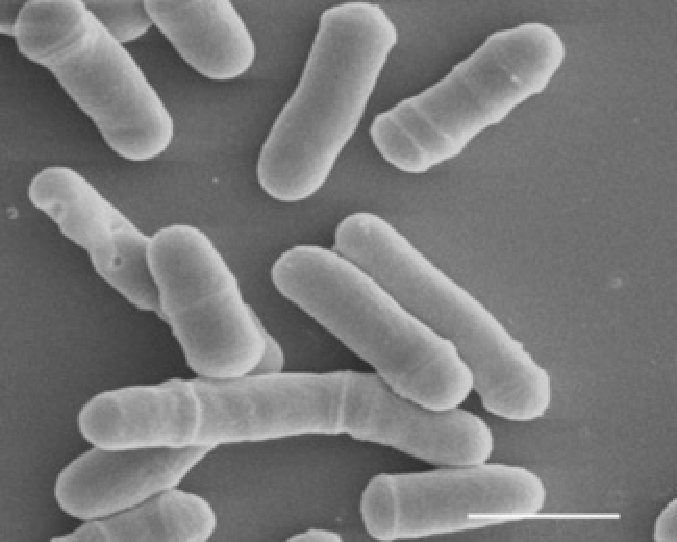
\includegraphics[width=0.5\linewidth]{fissionYeast}
    \caption{Microscopic view of a fission yeast culture. The scalar bar indicates $10$ $\mu$m. Image reprinted from \cite{Morgan2007} with permission. }
    \label{fig:fissionYeast}
\end{figure}

Fission Yeast is widely used in traditional brewing and baking. It was first discovered in 1893 in the sediment of millet beer \cite{Fantes2016,Hoffman2015}. As a single-celled fungus, fission yeast has a simple genome with three different chromosomes. The genome of fission yeast is fully sequenced and the three chromosomes contain about $14$Mb of DNA \cite{Wood2002}. It has a rapid growth rate and easily manipulated to make mutants, which make it a perfect modeling organism for genetic studies. The growth of the fission yeast is simply by the elongation at the ends. After mitosis, division occurs by the formation a cell plate that cleaves the cell at its midpoint \cite{Forsburg2003}. 

Fission yeast is normally a haploid cell. However, when put under stressful conditions, such as nitrogen deficiency, two cells will conjugate to form a diploid and then form four spores via meiosis \cite{Coelho2013}. This is easy to observe experimentally and this stage is exactly when the interesting nuclear oscillation happens \cite{Chikashige1994}. In the next subsection, we will explain the basis of the meiosis in fission yeast. 



\subsection{Basis of meiosis}
\label{sub:basis_of_meiosis}

Meiosis is a kind of cell division that reduces the number of chromosomes in the parent cell by half and produces four genetically distinct gamete cells. This process occurs in all the sexually reproducing organisms, including human \cite{Freeman2008}. 

Meiosis begins with a parent cell with two copies of each chromosome, and is followed by two rounds of cell divisions which produce four potential daughter cells, each has half number of chromosomes as their parent cell. The two rounds of cell division are called \emph{Meiosis I} and \emph{Meiosis II}, respectively. It is during Meiosis I that the pair of chromosomes, one from the father and the other from the mother, separates into two offspring cells. Meiosis II is very similar to the mitosis where two sister chromatins separate \cite{Freeman2008,Villeneuve2001a}. See an overview of meiosis in Fig. \ref{fig:meiosis}.

\begin{figure}[htpb]
    \centering
    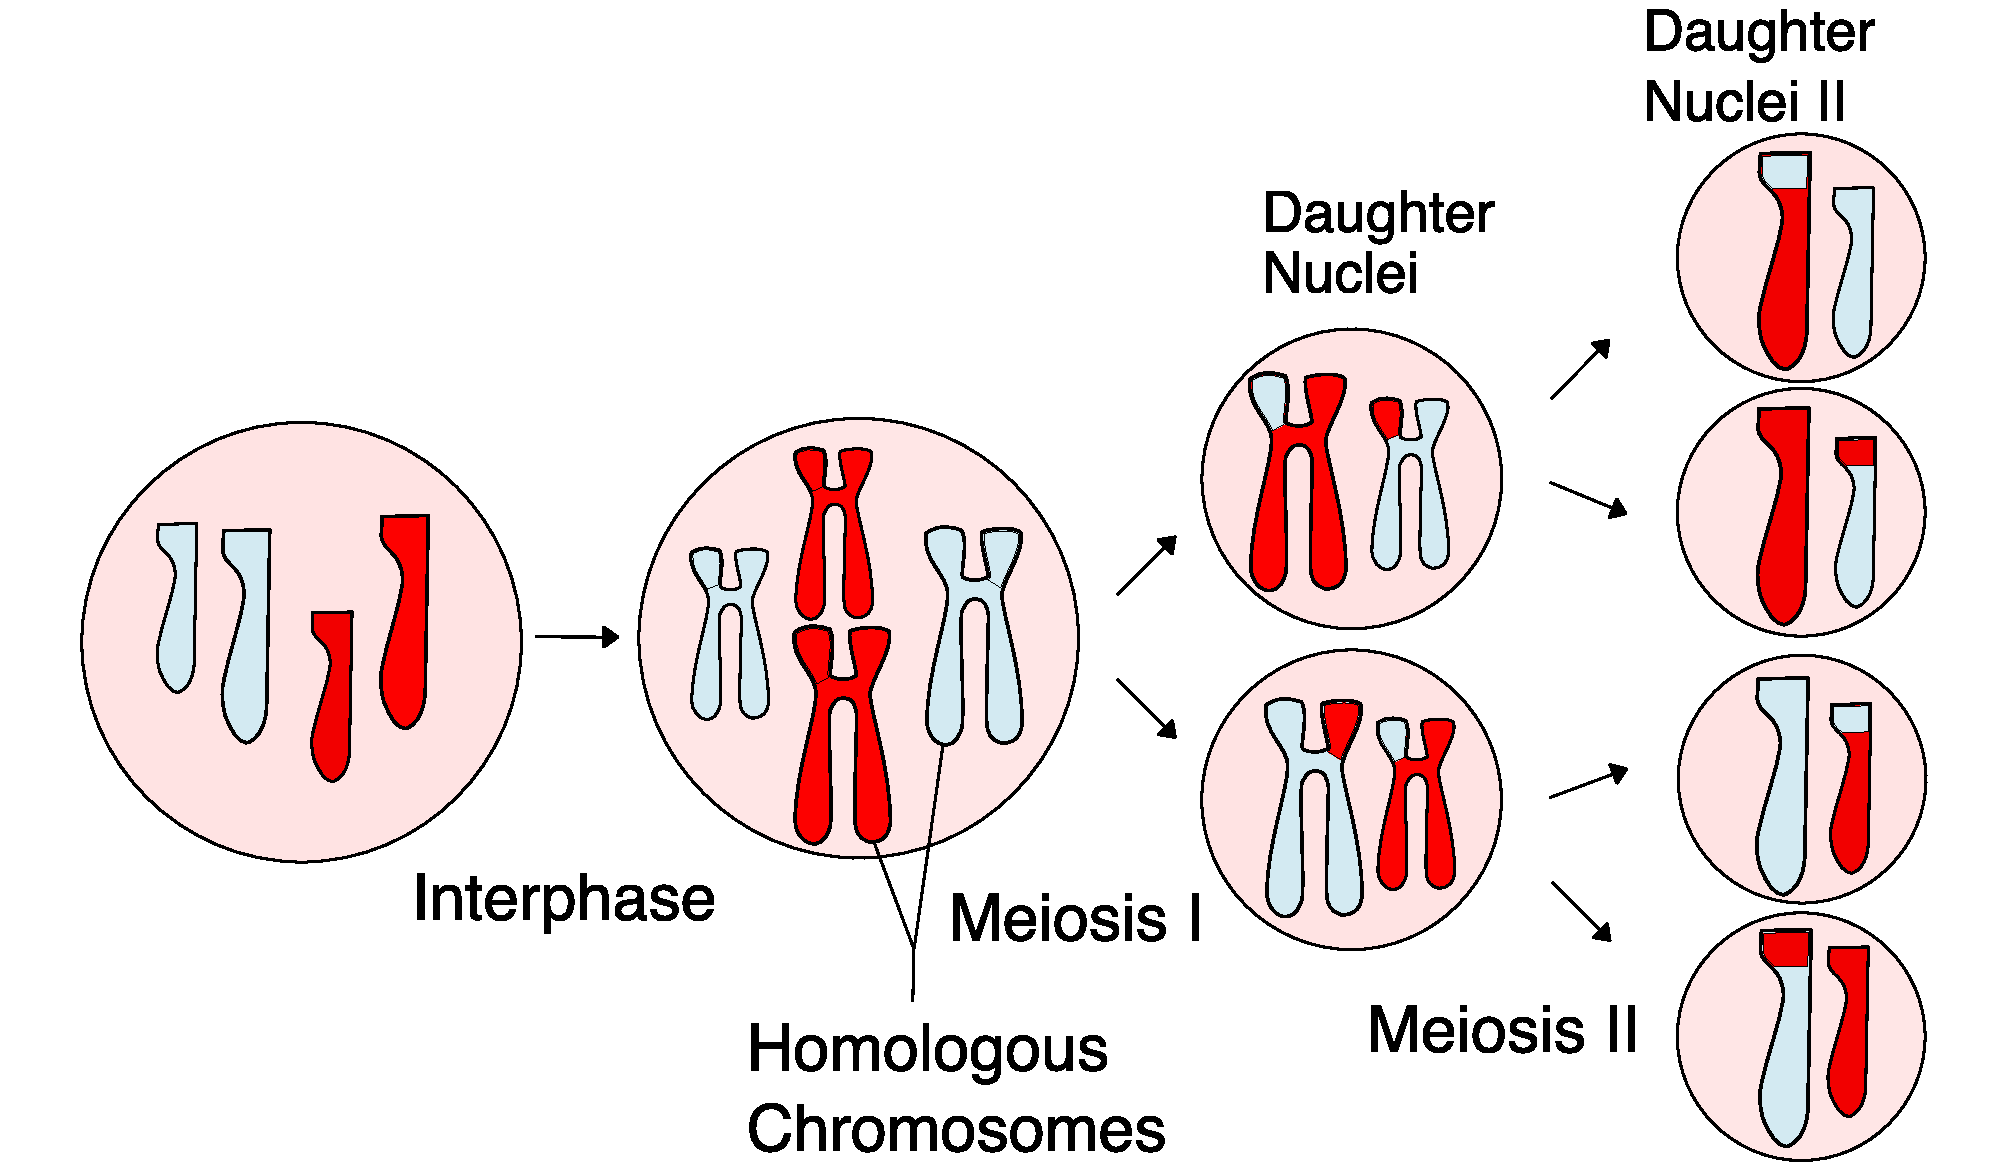
\includegraphics[width=0.8\linewidth]{meiosis}
    \caption{Overview of meiosis and an illustration of recombination between homologous chromosomes resulting in four unique daughter cells. Image reprinted from \cite{} with permission.}
    \label{fig:meiosis}
\end{figure}

As in mitosis, each round of cell division can be divided in prophase, metaphase, anaphase, and telophase. We will elaborate Meiosis I in details, especially the Prophase I when the nuclear oscillation happens. 

\emph{Prophase I}: prophase I is an important stage that many processes happened. Two of the examples are bouquet formation \cite{Wegener1980a} and homologous recombination \cite{Davis2001,Gerton2005}, both occurring in generic organisms. In the early state of Prophase, chromosomes are reorganized spatially, usually, the telomeres are clustered and attached to a small region of the nuclear membrane, forming a bouquet structure. This is called bouquet formation or telomere clustering in biology \cite{Chikashige1994,Wegener1980a,Niwa2000}, see in Fig \ref{fig:prophase} for an example in fission yeast. In the process of recombination, the homologous chromosomes, which are paternal and maternal pairs, align and exchange some parts of their DNA and usually results in the chromosomal crossover. Homologous recombination is critical for pairing and accurate segregation of the chromosomes in the later stage of Meiosis I. More interestingly, this stage is exact the period when the nuclear oscillation happens in fission yeast \cite{Ding1998,Wells2006}. We will devote this part to next subsection.

\begin{figure}[htpb]
    \centering
    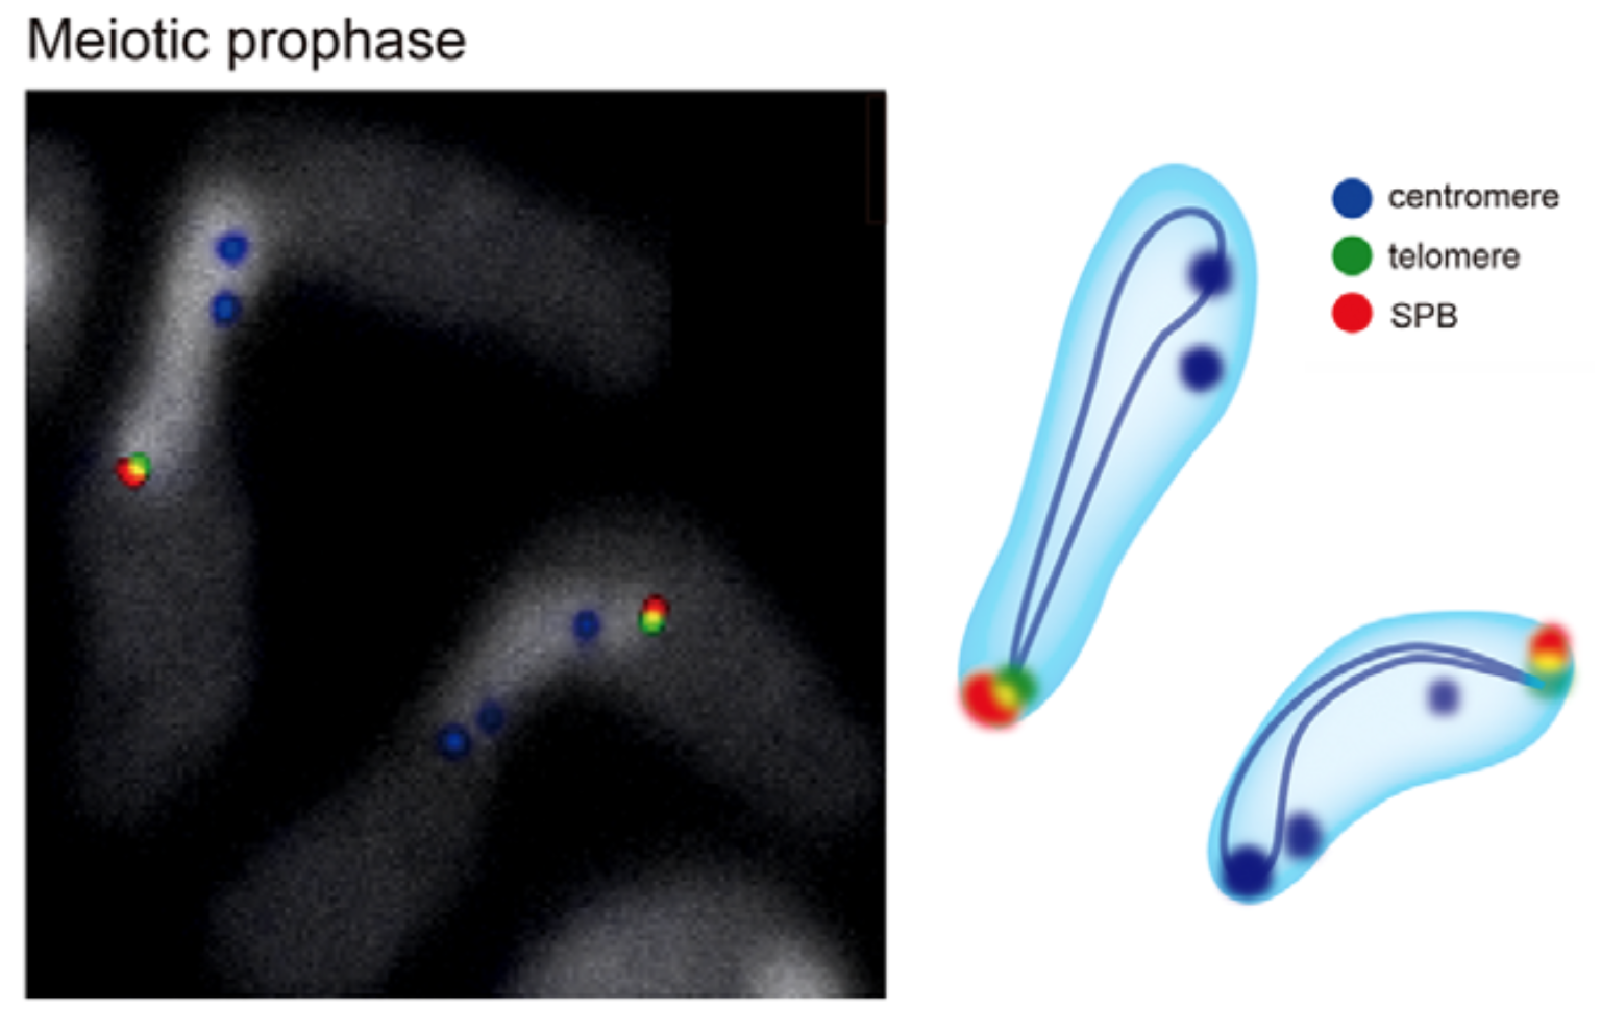
\includegraphics[width=0.8\linewidth]{prophase}
    \caption{The meiotic prophase I of fission yeast. Telomeres are clustered to form a bouquet structure. Image modified and reprinted from \cite{Asakawa2007}.}
    \label{fig:prophase}
\end{figure}

\emph{Metaphase I}: in this stage, homologous pairs move together along the middle plate, the microtubules from centrosomes attach to their respective chromosomes, the paired homologous chromosomes align along an equatorial plane that bisects the spindle. However, in Fission Yeast, the centromere is replaced by a functional equivalent organelle called spindle pole body (SPB) \cite{Freeman2008}.

\emph{Anaphase I}: in this stage, the microtubules shorten, pulling homologous chromosomes to opposite poles. Notice here, chromosomes still consist of a pair of sister chromatids. The cell body elongates, preparing for cell division \cite{Freeman2008}.

\emph{telophase I}: in the last stage of Meiosis I, chromosomes arrive at the poles. The microtubules network of spindle disappears. New nuclear membrane appears. The two daughter cells now only have half the number of chromosomes \cite{Freeman2008}.

After Meiosis I, Meiosis II occurs without DNA replication in between. The process is similar to Meiosis I except the sister chromatids segregate instead of homologous chromosomes \cite{Freeman2008}. Four unique daughter cells are formed after the completion of Meiosis. The homologous recombination process takes an important role for this uniqueness.

\subsection{Nuclear oscillation}
\label{sub:nuclear_oscillation}

As mentioned in the previous subsection, nuclear oscillation happens during prophase I of meiosis in fission yeast, and so as the important processes of chromosomes homologous alignment and recombination \cite{Ding1998}. Because the impressive shape of nucleus during this stage, nuclear oscillation also often mentioned as \emph{horse-tail} movements in biology\cite{Koszul2009a,Wells2006,Davis2001}, see in Fig. \ref{fig:oscillation} for a time-lapse illustration. We believe the chromosome movements play an important role in this process and decide to model it quantitatively. In this subsection, we are going to elaborate the details of nuclear oscillation. We will answer the questions like what is the internal structure of nucleus during oscillation, what is the driven force of the oscillation, how long the oscillation lasts and what is the time period of the oscillation, etc.
\begin{figure}[htpb]
    \centering
    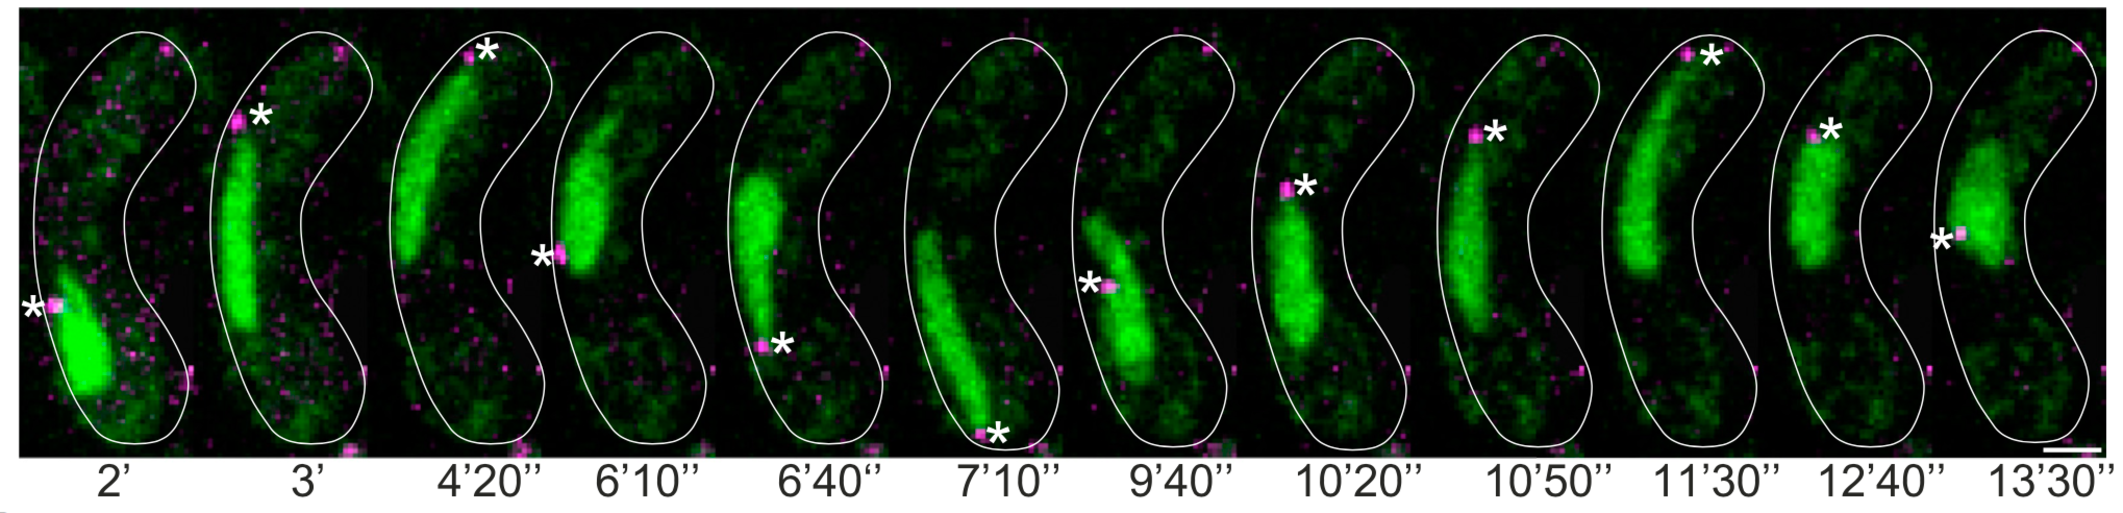
\includegraphics[width=1.0\linewidth]{oscillation}
    \caption{Time-lapse experiments of nuclear oscillation in fission yeast, DNA marker in green (Rec8-GFP) and SPB marker in magenta (Sid4-mCherry) also indicated by asterisk. Reprinted from \cite{Chacon2016} with permission.}
    \label{fig:oscillation}
\end{figure}

\emph{The looping structure of chromosomes}: before the nuclear oscillation, chromosomes are reorganized and the bouquet formation happens. In fission yeast, the SPB is anchored in the nuclear envelope, telomeres of chromosomes are clustered to the SPB region of the inner nuclear membrane. The chromosomes are condensed to be the rod-like chain. Notice that there are still two sister chromatins contained in one chromosome. With all the telomeres bond to the SPB, chromosomes form the looping structure, as we can see in Fig. \ref{fig:prophase}. 

\emph{Redistribution of dynein motors drives the nuclear oscillation}: while the inner side of SPB bonds the chromosome telomeres, the outer side is attached to the microtubules in the cytoplasm. During the oscillation, dynein motors are the energy supplier. Interestingly, as one motor is not enough for the oscillation, the collective behavior of motors is observed to drive the nucleus motion. The spatial distribution of motor molecular varies during the oscillation. Motors accumulates in the side of fission yeast that the nucleus moves toward to. It is found that the pulling force is the main contribution that drives the oscillation \cite{Vogel2009}.

\emph{Related biological parameters of nuclear oscillation}: to study the dynamics during oscillation, several parameters are estimated experimentally and input into our model later. These parameters are summarized in table \ref{tab:parameters}.

\begin{table}[htpb]
    \centering
    \caption{Parameters of fission yeast during meiosis}
    \label{tab:parameters}
    \begin{tabular}{l|l}
        \hline
        \textbf{Parameter} & \textbf{Value} \\
        \hline
        Typical size of nucleus          &  $3\mu$m \\
        Chromosome number                &  Three pairs \\
        Compaction ratio of chromatin    &  $10^2$bp/nm \\
        Kuhn length of chromatin         &  $100\sim300$nm  \\
        Duration of nuclear oscillation  &  $2$ hours  \\
        Period of nuclear oscillation    &  $10$ min  \\
        Moving speed of nucleus          &  $2.5\mu$m/min \\
        Viscosity of nucleoplasm         &  $1000\times \mu_{\text{water}}$ \\
        \hline
    \end{tabular}
\end{table}


\subsection{The role of nuclear oscillation}
\label{sub:the_role_of_nuclear_oscillation}

Although we can clearly observe the nuclear oscillation in fission yeast, the biological role of it is not thoroughly understood. One intuitive hypothesize is that the movement facilitates the paring of homologous \cite{Ding2004}. However, Koszul et al. proposed that the chromosome movement might play other roles than paring, such as resolve homologous entanglements or non-homologous connections \cite{Koszul2009a}. Also, Mariola et al. stated a dual role for the nuclear oscillation, promoting initial paring and restricting the time of chromosome associations to ensure proper segregation \cite{Chacon2016}. 

We believe nuclear oscillation plays an important role for the chromosome alignment. However, it is hard to image the exact mechanism of the alignment without going deeper of the process. That is why we propose a quantitative model in this thesis and study the statistical and dynamical details of the model, trying to understand to the machinery of paring quantitatively. 


%********************************** %Second Section  *************************************
\section{Chromosomes modeled as the polymer}
To quantitatively describe the chromosome, it is natural to model it as a polymer. In fact, there are already a lot of excellent examples in this direction \cite{Wong2013,Tree2013,Halverson2014,Jun2010a}. However, depending on the situations under considering, different polymer models may applied. 

In physics, a polymer model is usually described by beads connected by massless springs or rods. The interactions, usually characterized as different types of potentials, specify the setting of the model \cite{Doi1988}. As we want to model the chromosome during nuclear oscillation in fission yeast, there are two major factors we need to take into account besides some other minor details. First, the topology of the chromosome is a ring structure as shown in Fig \ref{fig:prophase}. Second, all chromosomes are bound to the SPB and pulled by an external force. According to these biological factors and the experimental measurements like Fig. \ref{fig:prophase}, we propose a pulled polymer loop model for the chromosomes in this specific situation. See in Fig. \ref{fig:schematic} for a sketch of our model. We will leave the discussion of the model details in afterward chapters.

\begin{figure}[htpb]
    \centering
    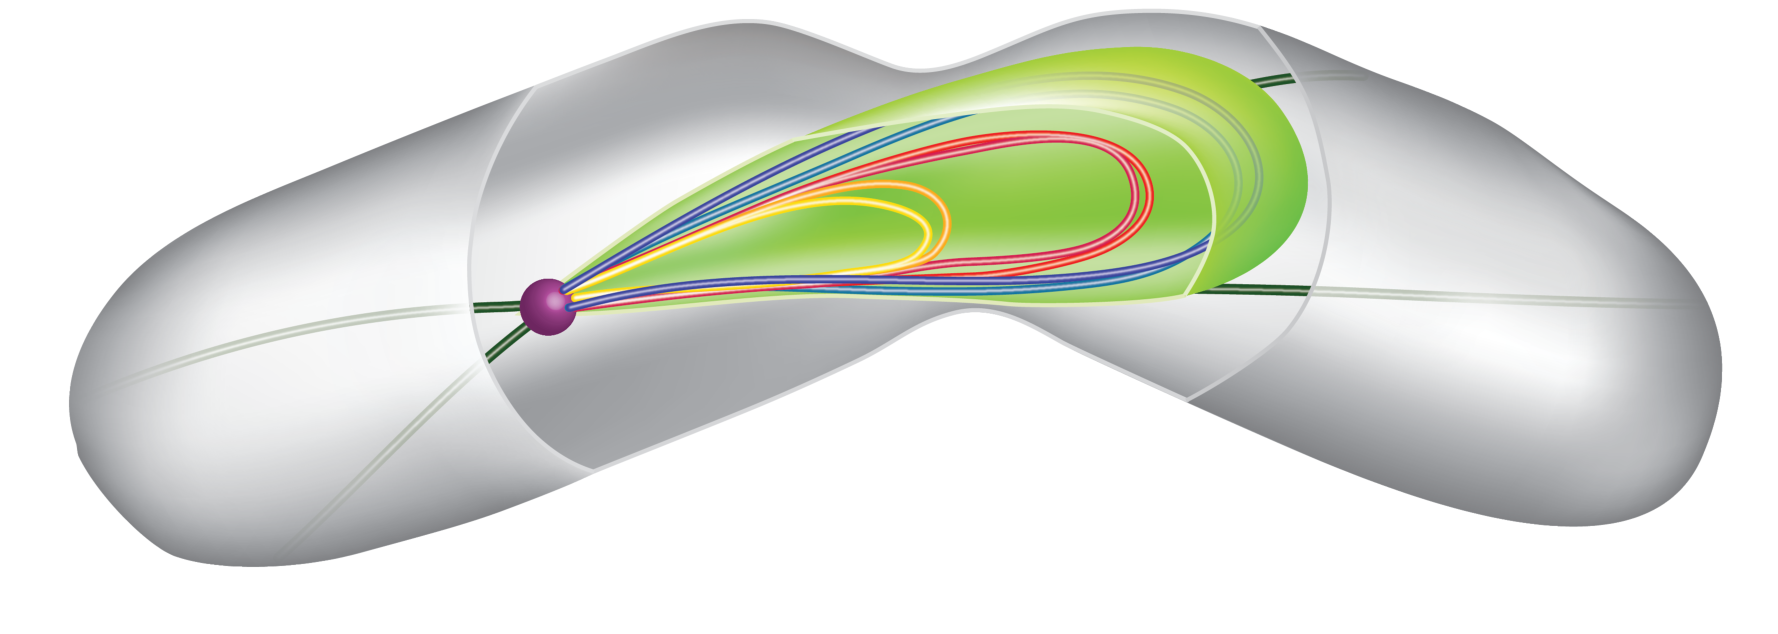
\includegraphics[width=0.8\linewidth]{schematic}
    \caption{The sketch of our pulled polymer loops model for chromosomes in meiotic fission yeast. Three pairs of chromosomes with all ends bound to SPB (shown in magenta) in the nucleus are indicated by different colors.  The SPB is pulled by multiple dynein motors (not shown) walking along microtubules (dark green). The SPB is anchored to the nuclear envelope (light green) and entrains the whole nucleus.}
    \label{fig:schematic}
\end{figure}

To the best of our knowledge, there are not many works which are discussing on not only the polymer loops but also the polymer is pulled by an external force. In the following subsections, we will introduce two related aspects of previous works, i.e. works about the polymer loops and works related to pulled polymer. 

\subsection{The ring polymer model}
\label{sub:the_ring_polymer_model}

Polymers forming a ring structure are ubiquitous in chemistry and biology \cite{Halverson2014,Richter2015}. The study of ring polymer can go back to the years when polymer physics was built up \cite{Kramers1946,Zimm1949}. Kramers developed an equilibrium theory that possesses branch points and rings of the dilute polymer solution in 1946 \cite{Kramers1946}. Zimm calculated the statistics of mean square radii of molecules containing branches and rings in 1949 \cite{Zimm1949}. However, comparing to the simplest polymer chain model, research focus on polymer ring are far less than the former. We will review here some interesting and most related ones. Of course, it is not possible to exhaust all related works here, we pay our attention particularly to those that are related to the chromosome modeling.

Since Kramers and Zimm, there are a number of works trying to study the static and dynamical properties of the ring polymer from the theoretical point of view.
In 1965, Casassa derived some statistical properties of flexible ring polymers, including mean square radius, the second Virial coefficient and angular distribution of scattering \cite{Casassa1965}. 1980, Burchard and Schmidt calculated the static and dynamical structure factors of flexible ring polymers \cite{Burchard1980}. Baumg\"{a}rtner considered the self-avoiding effect of ring polymers in 1984 and found the asymptotic scaling exponents are the same as linear polymers \cite{Baumgartner1982a}. In 1986, Cates et al. studied the nor-concatenated ring polymer melt and found the size of polymer $R$ scales with the polymerization index $N$ as $R\sim N^{2/5}$ and the diffusion constant $D$ scales as $D\sim N^{-2}$ \cite{Cates1986}.  In 1994, Obukhov et al. considered the dynamics of a ring polymer in a gel and obtained the diffusion coefficient scales with the molecular weight as $D\sim M^{-2}$ and the longest relaxation time $T$ scales as $T\sim M^{5/2}$ \cite{Obukhov1994}. Carl investigated the configurational and rheological properties of multiple-twisted ring polymers using a long cyclic finitely extensible bead-spring model in 1995 \cite{Carl1995}. He also presented a study on bead-spring chains in steady flows, various properties such like the power spectrum, the autocorrelation functions of configurational quantities were discussed in 1996 \cite{Carl1996}.
In 2001, Panyukov and Rabin studied the effects of thermal fluctuations on elastic rings. Analytical expressions are derived for some static and dynamical quantities \cite{Panyukov2001}.  Mukherji et al. studied a polymer ring or chain diffused around attractive surfaces. They found the diffusion constant scales as $D \sim N^{-3/2}$ linear chain and solid strong adsorbed surfaces, and $D\sim N^{-1}$ for ring polymer and soft surfaces in 2008 \cite{Mukherji2008}. Sakaue proposed a simple mean-field theory for the structure of ring polymer melts which takes into account the many-body effects \cite{Sakaue2011,Sakaue2012}. In 2012, Kim et al. presented a self-consistent field theory formalism of topologically unconstrained ring polymers \cite{Kim2012}.  In 2013, Reigh performed lattice Monte-Carlo simulations to investigate the dependence of ring polymer conformation to the concentration, where the scaling of gyration radius with the concentration $R_g \sim \phi^{-0.59}$ was found \cite{Reigh2013}. In 2014, Lang et al. studied the tumbling dynamics of semiflexible ring polymers as a model of the cytoskeletal filament in a shear flow. They found the tumbling frequency scales $f_c$ scales with the Weissenberg number as $f_c \sim Wi^{3/4}$ rather than the prediction of classical theory that $f_c \sim Wi^{2/3}$ \cite{Lang2014b}.

Ring polymer with high concentration, like polymer melts, are often used in modeling interphase chromosomes. Interestingly, it is found that during interphase, the spatial organization for the multiple chromosomes in the nucleus is not homogeneous and well mixed. Instead, each chromosome forms its own ``territories'' \cite{Halverson2014}. Many interesting works can be found respecting to this problem. For example, in 2008, Rosa and Everaers used the simulation results of polymers to explain the existence and stability of territories of interphase chromosomes in genetic eukaryotes \cite{Rosa2008}. Because usually, the computation power required to simulate the whole genome is huge, they also developed an efficient multiscale numerical approach to study the conformational statistics of ring polymers melts in \cite{Rosa2014b}.  Dorier employed a very simple non-permeable freely jointed polymer model and recovered the chromosomal territories in a crowded nuclei \cite{Dorier2009}. This part of work is well reviewed in \cite{Halverson2014}, the interested reader can refer to the references therein. 

On the other hand, it is also possible that ring polymer structures are formed temporarily in chromosomes. This could be caused by the DNA replication process or binding proteins connecting two loci of chromosomes. Many great works were done also in this direction. In 1995, Sachs use a looping random walk model to study to the interphase chromosomes, fluorescence labeled data is compared to the theoretical prediction \cite{Sachs1995}. Marko considered a model of two polymer rings tethered one another and its application to chromosome segregation in 2009 \cite{Marko2009}.  The looping probabilities of interphase chromosomes were also discussed in \cite{Rosa2010}.  In 2011, Zhang et al. modeled the meiotic chromosomes as a polymer that could form internal loops by binding proteins. They found the loops play an important role in the mechanical properties of the polymer \cite{Zhang2011a}. Wong set up a polymer model and use it to predict the whole nuclear architecture of fission yeast \cite{Wong2012}. Dekker and Giorgetti employed the computational polymer model to explain the 3C/HiC data \cite{Dekker2013,Giorgetti2014}. In 2014, Youngren employed ring polymer model to study the duplication and segregation of \emph{E. coli} chromosomes \cite{Youngren2014}.  These are just a few examples, more can be found if one is interested.

The confinement such as the nuclear membrane or cell shape could also take an important role in chromosome dynamics. One of the examples of this kind of work is Fritsche's work in 2011, they studied the influence of confinement geometry to the spatial organization of semiflexible ring polymers \cite{Fritsche2011}. The studies of the polymers (including chains and rings) under confinements were reviewed by Ha el al. in \cite{Ha2015}. 

There are also a lot of great experimental work related to ring polymers. In 1992, Tead et al. employed polystyrene molecules to perform experiments and compared the diffusion of linear and ring polymers \cite{Tead1992}. Kapnistos et al. found the stress relaxation of entangled ring polymer was power-law rather than exponential in \cite{Kapnistos2008}. Structure and dynamics of polymer rings by neutron scattering were studied by Br\'{a}s et al. in 2011. Witz et al. employed the atomic force microscopy to studied 2D circular DNA in \cite{Witz2008,Witz2011}.  Goo{\ss}en et al. studied dynamics of polymer rings using neutron spin echo spectroscopy which space-time evolution of segmental motion could be observed \cite{goossen2014,Goossen2015}. 

Due to its importance, the study of ring polymers is much intensive and causes much more attention nowadays. Besides what we have mentioned above, the shape of ring polymers is studied in \cite{Bishop1985,Jagodzinski1992,Alim2007,Reiss2011}. Also, there are a series of works considering the ring polymer with entanglements and topological knots \cite{Michels1982,Polymers1991,Koniaris1991,Grosberg1996,Shimamura2001,Orlandini2003,Tubiana2011,Uehara2014,Li2015a}.
We are only able to list a few of those great works. Interested readers can refer to the references therein. 

\subsection{Pulled polymer model}
\label{sub:pulled_polymer_model}

As we mentioned above, in order to model the nuclear oscillation of fission yeast, we have to consider the pulling dynamics. If we transfer the coordinate and sit on the pulled monomer, a pulled polymer is also equivalent to a pinned polymer in an external flow or force field. In this section, we would like to review some previous works in this direction. Most of them are about pulled polymer chain. Whatsoever, we think it is still helpful to know what have been done about pulled polymers or tethered polymer in an external field.

A polymer chain with one end free and the other end pulled by an external force was first discussed by de Gennes \cite{DeGennes1974,DeGennes1979}. After that, another important progress was made by Pincus, he developed what is now called Pincus theory \cite{Pincus1976,Pincus1977}, which consider the pulled polymer as a sequence of independent ``blobs''.  Brochard-Wyart further developed the ``trumpet'' and the ``stem-flower'' pictures of pulled polymer chain \cite{Brochard-Wyart1993a,Brochard-Wyart1994a,Brochard-Wyart1995,Adjarei1995a}. When the pulling force is not too strong, the polymer presents as a series of independent blobs with increasing size, i.e. the portion of polymer near to the free end fluctuates more. As the pulling force increased to a strong regime, the polymer portion near to fixed end is totally stretched, forming a ``stem-flower'' like picture, see in Fig. \ref{fig:stemFlower}.  
Using fluorescence microscope and optical tweezers,  Perkins et al. performed the pulling experiments on single DNA molecule and found the results consistent with the Brochard-Wyart's theory \cite{Perkins1995a,Perkins1994}. They also measured the relaxation time of this pulled polymer and obtained the scaling $\tau \sim L^{1.66}$ \cite{Perkins1994a}. Wirtz also confirmed the theory by measuring transport properties of a single DNA molecule in \cite{Wirtz1995}.

\begin{figure}[htpb]
    \centering
    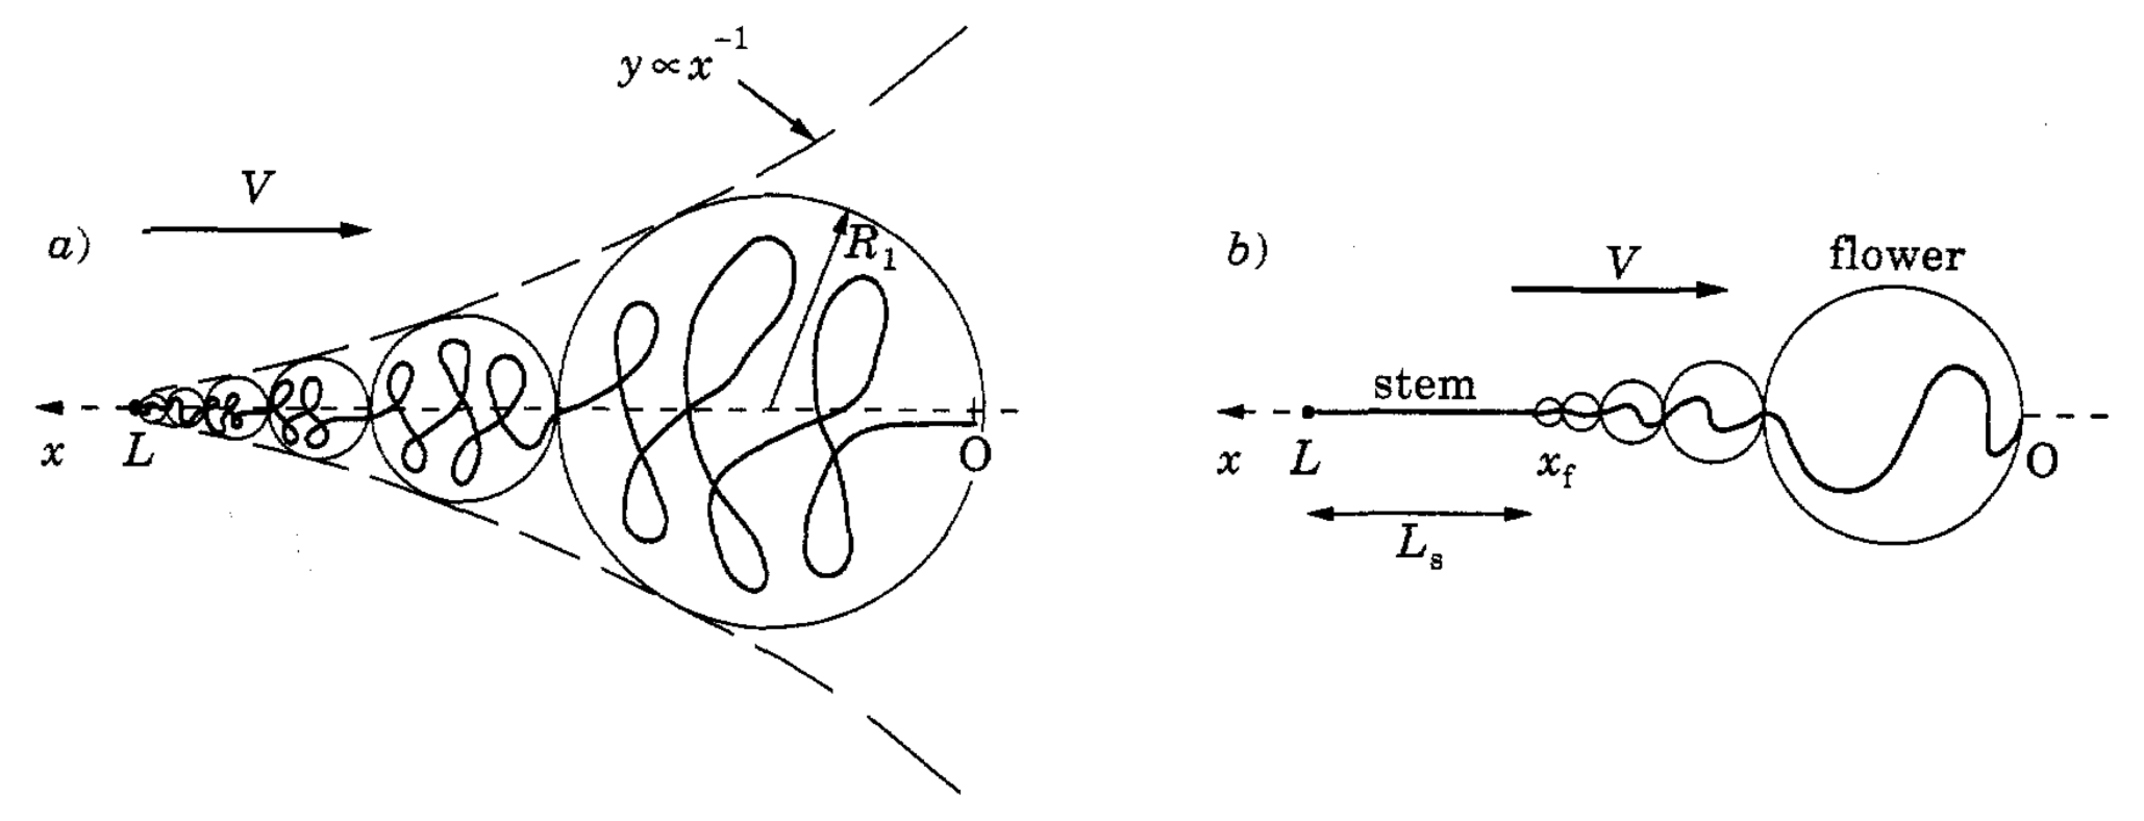
\includegraphics[width=0.8\linewidth]{stemFlower}
    \caption{Illustration of ``stem-flower'' picture for pulled polymer chain. (a) Trumpet picture at moderate pulling force; (b) Stem-flower picture at strong pulling force. Image reprinted from \cite{Brochard-Wyart1995}.}
    \label{fig:stemFlower}
\end{figure}


Rezehak et al. considered pinned polymer in a uniform flow with hydrodynamic interaction and proposed a so-called f-shell blob model \cite{Rzehak1999}. Larson et al. performed Brownian Dynamics simulation for a DNA in an external flow field \cite{Larson1999}. In 2000, Doyle measured the cyclic and stretching dynamics of a tethered DNA molecule in the shear flow \cite{Doyle2000, Ladoux2000a}. Sebastian studied the dynamics of pulling a polymer out of a potential well \cite{Sebastian2000}. Cui performed the stretching and releasing experiment by pulling a single chicken erythrocyte chromatin fiber with the optical tweezers \cite{Cui2000a}. Rzehak discussed the conformation fluctuation and relaxation of a tethered polymer in uniform flow \cite{Rzehak2003a}. In 2007, Mohan et al. employed Rouse theory to study the unraveling dynamics of tethered semiflexible polymer in uniform solvent flow \cite{Mohan2007}. Sing et al. studied flexible and semiflexible tethered polymers in the limit of high shear flows and consequently near-full extension of the chains in \cite{Sing2011}.  Sakaue et al. studied the conformation and dynamics of a single flexible polymer chain that is pulled by a constant force applied at its one end, finite extensibility, the excluded volume, and the hydrodynamic interactions are discussed \cite{Sakaue2012a}.  Varghese et al. investigated the force fluctuations in stretching a tethered polymer \cite{Varghese2013}.
In 2013, Dai and Doyle found in \cite{Dai2013a} that the scenario of a pulled polymer is very similar to a polymer confined in a cylinder with proper radius.

To the best of our knowledge, the discussion of pulled ring polymer is missing except our own work \cite{Lin2015}. So we reviewed here the works about ring polymer on one side and the works of pulled polymer on the other side. Of course, the details are not shown here, interested readers can go into the references.

%********************************** %Third Section  *************************************
\section{Outline}  %Section - 1.3
\label{sec:outline}
With the introduction of the biological problem and the background of polymer modeling in previous two sections, we are ready to go into the details of our study. In this section, we will propose our research goals for this thesis and give an overview for the organisation of the thesis.

\subsection{Research goals}
\label{sub:research_goal}

The research goals of this thesis is listed as following:

1. Propose a polymer model to describe the chromosomes in fission yeast during nuclear oscillation. This is actually already mentioned in the previous section, i.e. the pulled polymer loop model. However, the details of the model will be discussed in the following chapters.

3. Develop the quantitative theory for our pulled looping polymer model. As far as we know, there is no previous work on this issue. On the other hand, it is shown by the experimental facts that this model is the best one for our problem. 

2. Perform realistic numerical simulations of the nuclear oscillation of fission yeast using the polymer model. The theory is always simplified and has a lot of assumptions in order to analytically tractable. It is necessary to do a realistic simulation that can verify our theory on one hand, and comparable to the experimental data on the other hand.

4. Using the physical insights to understand to biological processes such as chromosome alignment. Understand the biology is our ultimate goal. The chromosome movements during cell division are so important that many diseases are related to that, such as Down syndrome \cite{Patterson2009}. Our understanding from physical layer helps to fight with these diseases.

In one sentence, we want to quantitatively model the chromosome dynamics during the nuclear oscillation and use it to understand the biology. 

\subsection{Overview of the thesis}
\label{sub:organisation_of_the_thesis}

Add afterward.








%*******************************************************************************
%****************************** Second Chapter *********************************
%*******************************************************************************

\chapter{Theoretical Model and Numerical Simulation Methods}
\graphicspath{{Chapter2/Figs/}}

To model the chromosome movements during nuclear osculation in fission yeast, let us start from a single chromosome modeled by a single polymer loop. 
In this chapter, we will introduce the details of the polymer model for the chromosomes and the simulation methods that resolving the dynamics and statistics of the polymer. 


%********************************** %First Section  **************************************
\section{Stochastic models of polymer loops}
\label{sec:stochastic_models_of_polymer_loops}

As mentioned in the previous chapter, there are three pairs of chromosomes in fission yeast. During nuclear oscillation, these three pairs of chromosomes bound to one point, i.e. the Spindle Pole Body (SPB). Now let us start with the simplest case and neglect the interactions between chromosomes, think about a single chromosome. It is a polymer with the ring structure, and an external force is exerted on the SPB. We have two choices to model this chromosome, i.e. the bead-rod model or the bead-spring model. We will use both models in this thesis but more discussions are focused on the bead-rod. Both models have their own benefits and shortcomings. Computationally, it is easier to manipulate the bead-spring model than the bead-rod. However, the bead-rod has the intrinsic property of finite extensible without resorting to some complex nonlinear spring potentials. This benefit we think is important because the chromosomes are highly condensed and are definitely finite extensible. In fact, we will show that the finite extensibility takes an important role for the polymer dynamics, see in the later chapters. And the simplicity of bead-rod model offers us the possibility to find analytical solutions. 

In this section, we will introduce both the bead-rod and bead-spring model for modeling the chromosomes. However, before that, let us first do a coordinate transformation that makes our analysis much easier. 

\subsection{Coordinate transformation}
\label{sub:coordinate_transformation}
Let us consider a single chromosome pulled at the SPB. The pulling force drives the chromosome moves with a velocity $\mathbf{v}$. In our model, the SPB is modeled as one monomer in the polymer loop. Other monomers representing the chromosome move together with the SPB because of the bonds. This scenario of pulled polymer loop is shown in Fig. \ref{fig:coordinate} (a). 
\begin{figure}[htpb]
    \centering
    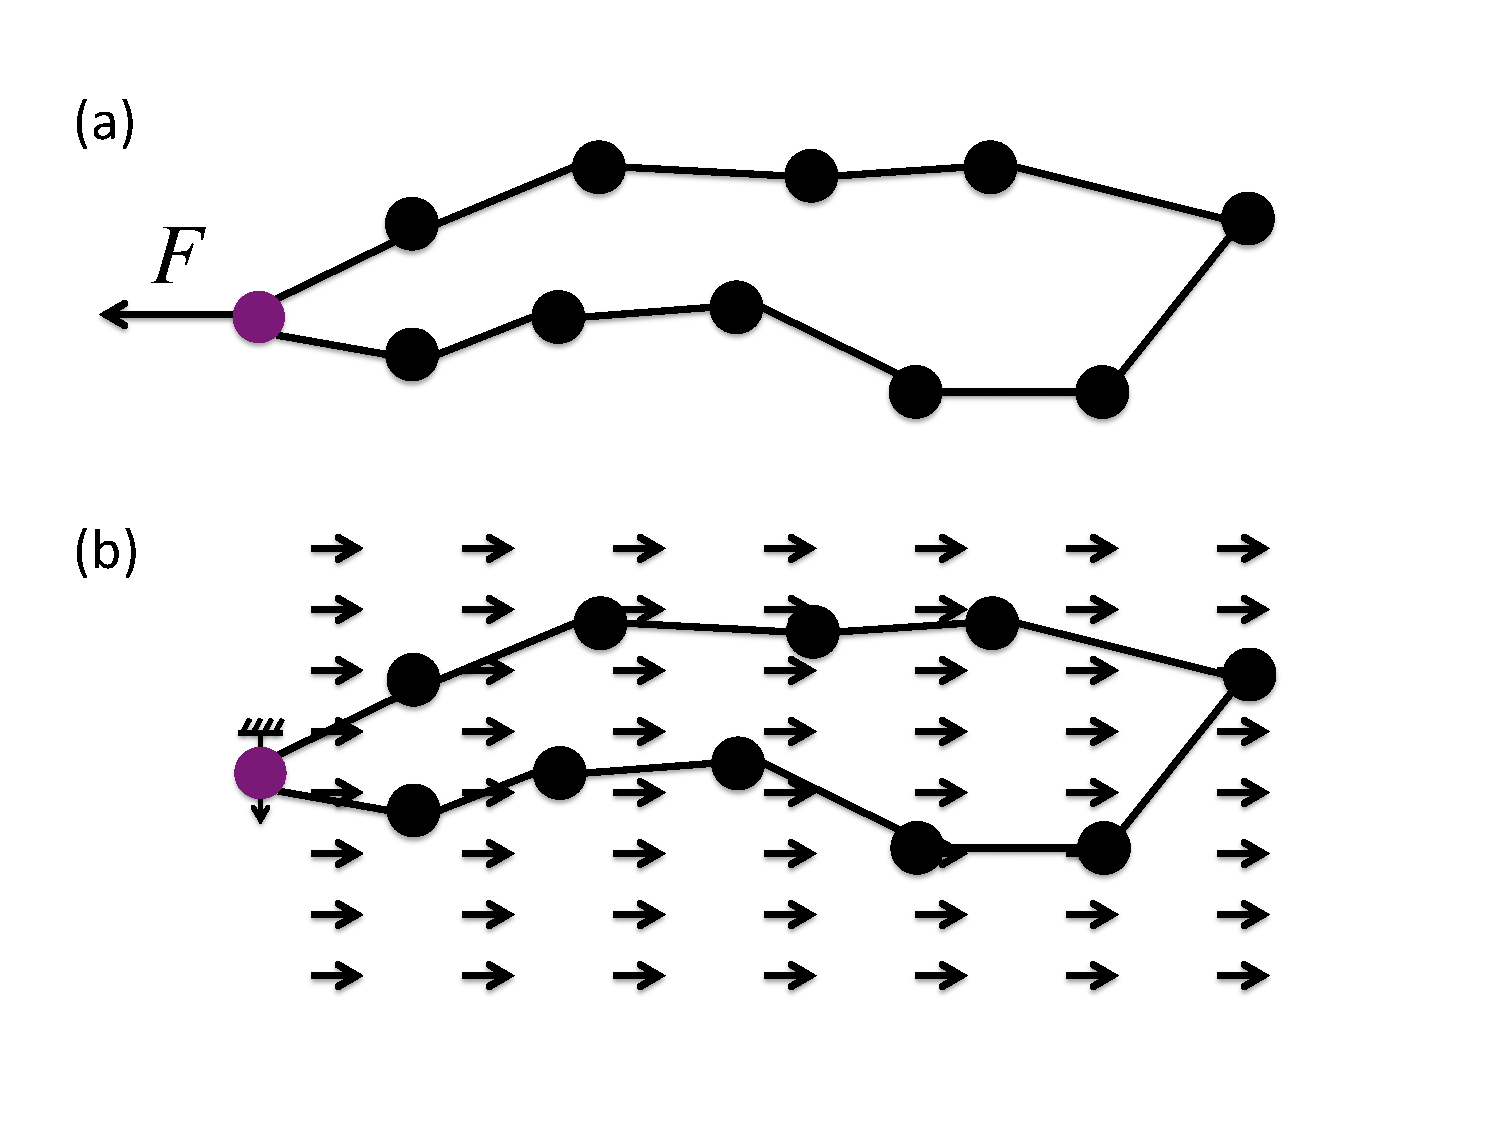
\includegraphics[width=0.8\linewidth]{coordinate}
    \caption{Illustration of coordinate transformation. (a) a pulled polymer loop before transformation; (b) pinned polymer loop in an external field after transformation. }
    \label{fig:coordinate}
\end{figure}

Now let us imagine we are sitting on the SPB. Then effectively, the SPB is pinned, and the polymer loop is immersed in a flow with velocity $-\mathbf{v}$, see in Fig. \ref{fig:coordinate} (b). Let us assume the Stoke's law is valid and according to that, there is a force $\mathbf{F}^e = - \xi \mathbf{v}$ exerting on every bead. $\xi$ is the friction coefficient for the bead in the solution.

In conclusion, the pulled polymer loop model is equivalent to the pinned polymer loop in an external force field. In our analysis, we will use the pinned polymer loop picture, because it is more easily to deal with both numerically and analytically. In the simulation, an extreme large pulling force is required if we use the first picture. The unusual force can easily become the bottleneck for the choosing of the integration time step. In theory, the force field picture offers a very clean energy landscape. Thus the pinned picture is preferred in out study. 

\subsection{Bead-rod model}
\label{sub:bead_rod_model}
Now let us come to a concrete polymer model for modeling the chromosomes, i.e. the bead-rod model. For this model, the beads representing chromosome segments are connected by the massless rigid rod. For simplicity, we assume the length of every rod is identical, denote by $a$. The rigidity of the rod means the distance between two neighboring beads is fixed. 
\begin{figure}[htpb]
    \centering
    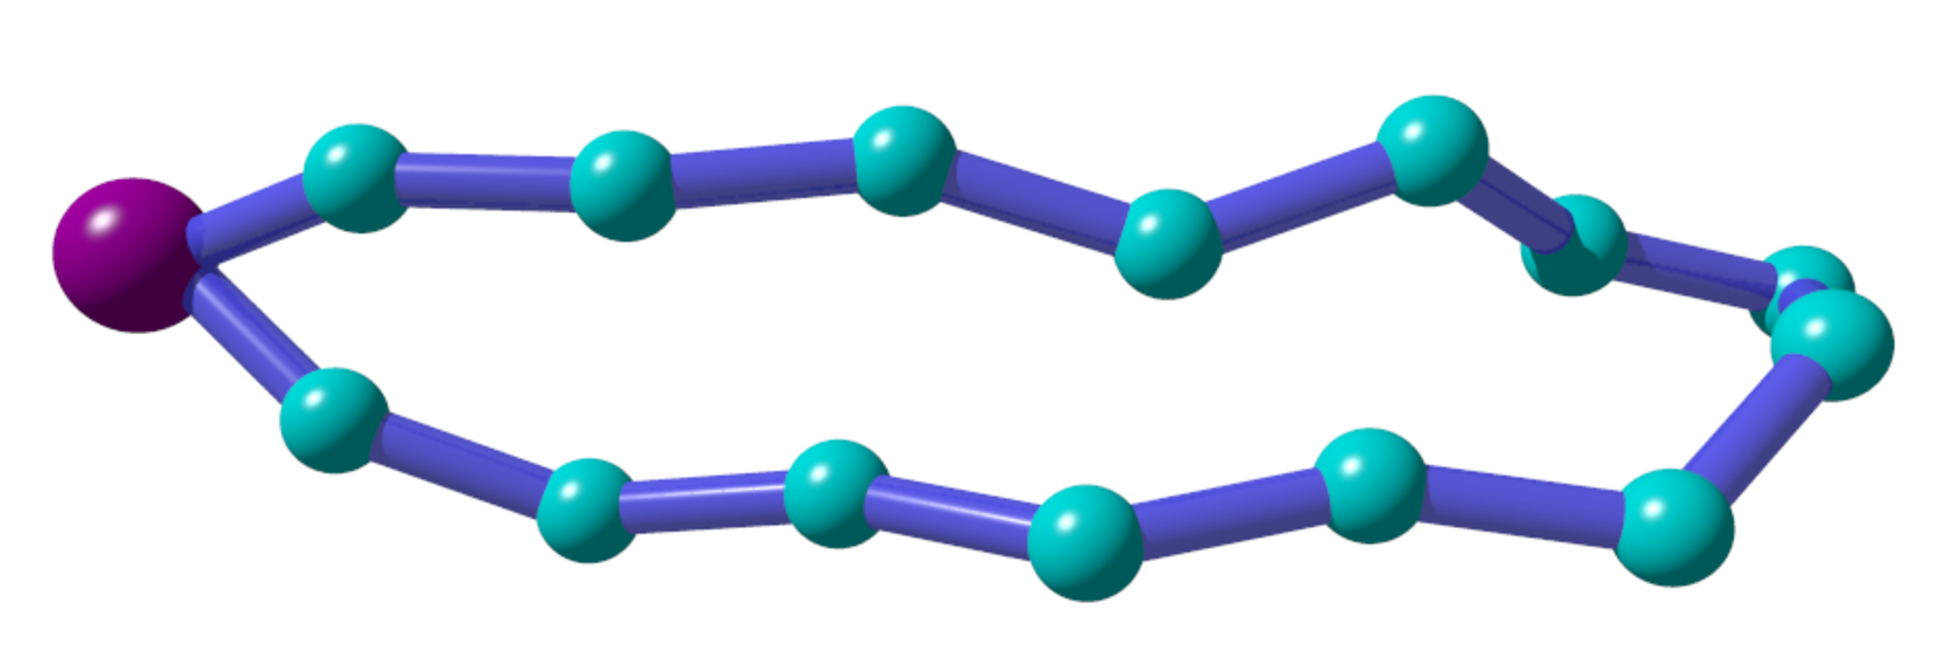
\includegraphics[width=0.8\linewidth]{beadrod}
    \caption{Sketch of the bead-rod loop model. The magenta bead represents the SPB and other cyan beads represent the chromosome segments.}
    \label{fig:beadrod}
\end{figure}

The dynamics of the polymer is specified by the motion of the beads. We shall first give out the dynamical equation and then explain how does it come from. Let us say the contour length of the polymer loop is $L$, i.e. there are $L$ beads (including the SPB) and $L$ rods in the polymer. Denote the beads by the index $i = 0, 1, 2,\cdots, L-1, L$. Notice that the periodic index is used due to the looping structure, i.e. for any indexing quantities $x_0 = x_L$. Then the dynamical equation of $i^{\rm {th}}$ bead can be written as
\begin{equation}
    \label{eq:beadrodEq}
    \xi \frac{d \mathbf{r}_i}{d t} = \mathbf{F}_i^{u} + \mathbf{F}_i^{c} + \mathbf{F}_i^{pseudo} + \mathbf{F}_i^{e} + \mathbf{F}_i^{b}
\end{equation}
where $\xi$ is the friction coefficient of the bead in the solution, $\mathbf{F}_i^{u}$ is the interaction force specified by some kind of potentials, $\mathbf{F}_i^{c}$ is the constraint force that keeps the rod length fixed, $\mathbf{F}_i^{e}$ is the external force and $\mathbf{F}_i^{b}$ is the Brownian force caused by thermal fluctuations. And what is left in the right hand of Eq. \eqref{eq:beadrodEq} is $\mathbf{F}_i^{pseudo}$, which is a special type of force introduced in the bead-rod model in order to get the correct statistics. We will discuss more about it later. 

Now let us come back to explain how does Eq. \eqref{eq:beadrodEq} come from.  Firstly, notice that $\mathbf{F}_i^b$ in the equation is a stochastic variable, so Eq. \eqref{eq:beadrodEq} is actually a stochastic differential equation. Secondly, the left-hand side of Eq. \eqref{eq:beadrodEq} is actually rearranged from the friction force of the bead in the solution $-\xi\mathbf{v}_i$. And we have assumed the solution is homogeneous so that the friction coefficient is independent of the space and time. Third, the inertial of the bead is neglected due to millions of collisions per second from the water molecules. In another word, Eq. \eqref{eq:beadrodEq} essentially can be written as $\mathbf{F}_i^{total} = \mathbf{0}$. This is simply the Newton's law with inertial neglected. This kind of dynamics is commonly used in polymer physics and called Brownian Dynamics \cite{Somasi2002,Cruz2012}. 

Let us now discuss each term of the right-hand side of Eq. \eqref{eq:beadrodEq} one by one. 

$\bullet$ Brownian force $\mathbf{F}_i^{b}$

The Brownian force can be caused by the enormous instantaneous collisions of the solvent molecules or by other sort of interactions between chromosomes and proteins in the nucleus. The level of fluctuation can be characterized by an effective temperature $T$. Mathematically, the Brownian force is described by a Gaussian process with the zero mean in space and time and the non-zero second moment, which can be written as:
\begin{subequations}
    \label{eq:brownianforce}
    \begin{equation}
        \left<\mathbf{F}_i^b\right> =\mathbf{0},
    \end{equation}
    \begin{equation}
        \left<\mathbf{F}_i^b(t)\mathbf{F}_j^b(t^{\prime})\right> = 2k_B T \xi \delta_{ij} \delta(t-t^{\prime}),
    \end{equation}
\end{subequations}
here, $\xi$ is the friction coefficient. $k_B$ is the Boltzmann constant. $\delta_{ij}$ is the Kronecker delta means there is no correlation for the Brownian force exerting on different beads. The second $\delta$ is the Dirac delta function. 

$\bullet$ External force $\mathbf{F}_i^{e}$

The external force in our pinned polymer loop model is simply the equivalent flow field after coordinate transformation. So we have $\mathbf{F}_i^e = \xi \mathbf{v}_{\rm{SPB}}$. In general, $\mathbf{v}_{\rm{SPB}} = \mathbf{v}_{\rm{SPB}}(t)$ is a function of time. However, when we consider the simplest case that the chromosome is pulled to move steadily in one direction, $\mathbf{v}_{\rm{SPB}}$ is a constant.

$\bullet$ Constraint force $\mathbf{F}_i^{c}$

The constraint force is the tension force on the rod to keep the length fixed. So the direction of the force is along the rod orientation. The rigid rod constraint can be written as 
\begin{equation}
    \label{eq:rodConstraint}
    |\mathbf{r}_{i} - \mathbf{r}_{i-1}| - a = 0,
\end{equation}
and $\mathbf{r}_{0} = \mathbf{r}_L$ for the periodic indexing. The constraint force is an implicit force that depends on the other force exerting on the beads. We will discuss how to calculate this force in next section. 

$\bullet$ \emph{Pseudo} force $\mathbf{F}_i^{pseudo}$

The \emph{Pseudo} force is a special virtual force that added in order to obtain the statistics we want. If we neglect the bending energy, excluded volume effect and other complex interactions in the model, we are essentially talking about the simplest freely joint polymer model. For such a simple model, we expect the random walk statistics, i.e. the orientation of two consecutive rods is independent. So the distribution of the included angle of two rods should be uniform. However, we cannot obtain this statistics as we want without the \emph{pseudo} force.

Let us take a simple example, the distribution of included angle of a trimer in 3D. Denote the angle as $\theta$. The 3D spherical uniform distribution can be written as
\begin{equation}
    \label{eq:trimerUniform}
    p(\theta) = const. \sin\theta.
\end{equation}
On the other hand, the distribution of rigid bead-rod trimer without \emph{pseudo} force can be derived using the generalized coordinate
\begin{equation}
    \label{eq:trimerRigid}
    p(\theta) = const. (1-\frac{1}{4}\cos^2\theta)^{1/2}\sin\theta.
\end{equation}
So they are not the same as we see here. The reason for this discrepancy is the rigidity of constraints reduce the phase space of the trimer from $6$ dimensional gully to $4$ dimension manifold. The simple Brownian force ensures the probability is uniform among the manifold but not $\theta$. 
\begin{figure}[htpb]
    \centering
    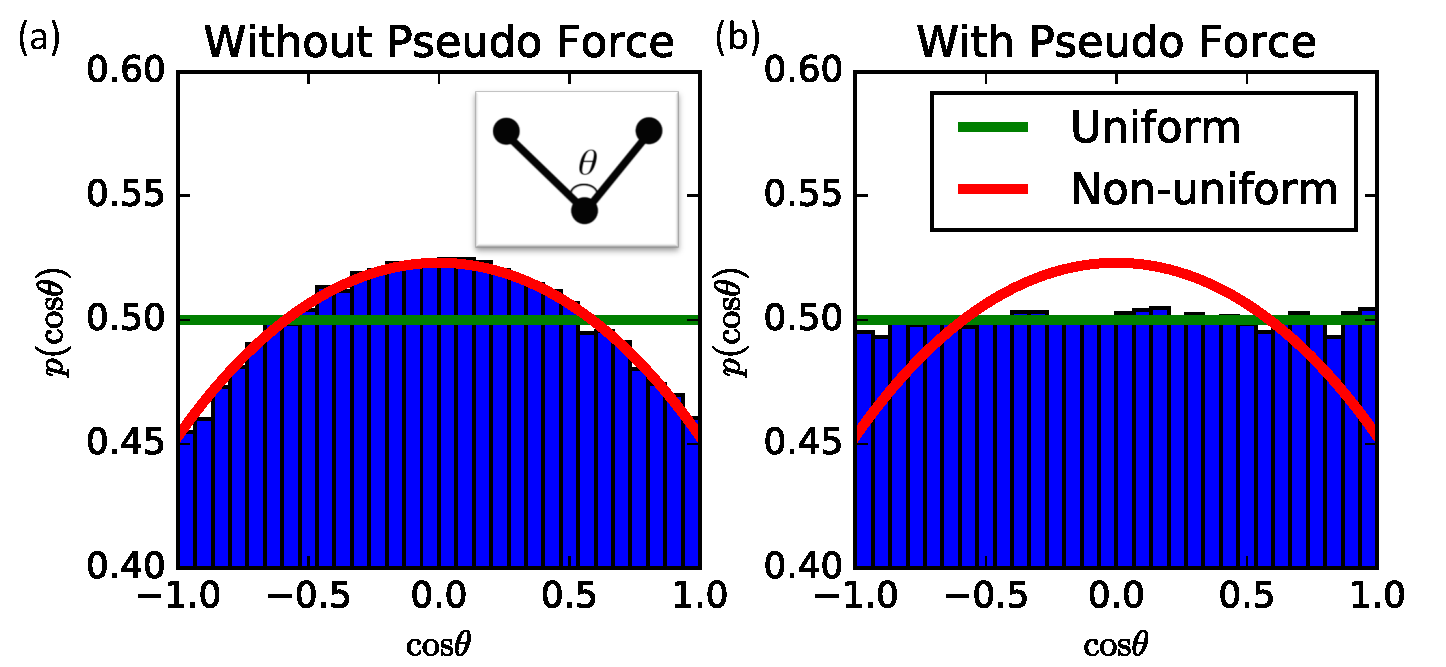
\includegraphics[width=1.0\linewidth]{trimer}
    \caption{The distribution of included angle of a bead-rod trimer. (a) without \emph{pseudo} force; (b) with \emph{pseudo} force. The blue bins are from Brownian Dynamics simulation results. Inset of (a) is a sketch for the trimer. }
    \label{fig:trimer}
\end{figure}

To solve the problem and obtain the statistics we want, Fixman introduced an effective \emph{pseudo} potential depends on the polymer configuration \cite{Fixman1974}, and hence we have a \emph{pseudo} force in Eq. \eqref{eq:beadrodEq}. The explicit form of the \emph{pseudo} force can be written as
\begin{subequations}
    \label{eq:pseudoForce}
    \begin{equation}
        \mathbf{F}_i^{pseudo} = -\frac{\partial U_{met}}{\partial\mathbf{r}_i},
    \end{equation}
    \begin{equation}
        U_{met} = \frac{1}{2}k_B T \ln(\det \mathbf{G}),
    \end{equation}
\end{subequations}
where $\mathbf{G}$ is the metric matrix of the bead-rod system \cite{Pasquali2002}. We will show the details for the calculation of \emph{pseudo} force in next section.

$\bullet$ Other potential forces $\mathbf{F}_i^{u}$

Other potential forces count the forces derived from bending energy, excluded volume effect, hydrodynamical interaction and other interaction potentials. The general form of this force can be written as
\begin{equation}
    \label{eq:potentialForce}
    \mathbf{F}_i^{u} = -\sum_{U}\frac{\partial U}{\partial\mathbf{r}_i},
\end{equation}
here $U$ can be different potentials. For instance, the bending potential can be calculated as 
\begin{equation}
    \label{eq:bending}
    U_{bend} = - \frac{\kappa}{a} \sum_{i=1}^{L} \mathbf{u}_i \cdot \mathbf{u}_{i-1}
\end{equation}
where $\mathbf{u}_i = (\mathbf{r}_{i} - \mathbf{r}_{i-1})/a$ is the unit vector of rod orientation, $\kappa$ is the bending stiffness and $a$ is the rod length.

For excluded volume effect, we usually model this interactive as pure repulsive Lennard-Jones potential
\begin{equation}
    \label{eq:lennardJones}
    U_{LJ} =  
    \begin{cases} 
        4\epsilon\left[\left(\frac{\sigma}{r}\right)^{12} -  \left(\frac{\sigma}{r}\right)^6\right],
        & \text{if } r \leq r_c; \\
        0,       & \text{if } r > r_c;
  \end{cases}
\end{equation}
where $r$ is the distance between two beads and $r_c = 2^{1/6}\sigma$, $\epsilon$ and $\sigma$ are two parameters.

One can add more interaction potentials into the model. However, adding more potentials could easily lead to a complex model with many parameters. For the sake of simplicity, we will actually ignore these forces in most of our analysis. See in our later chapters.


\subsection{Bead-spring model}
\label{sub:bead_spring_model}

Bead-spring model is another commonly used polymer model. There are several reasons that we use the bead-spring model complementary with the bead-rod model. First, the bead-spring model can work as a benchmark model of the bead-rod model. Unlike the bead-rod model, a \emph{pseudo} force have to be added to obtain the correct random walk statistics, the model of beads connected by Hookean springs is intrinsically a system satisfied the random walk statistics. Second,  the role of finite extensibility can be understood by comparing the bead-rod and bead-spring model. Third, the computation power needed for the bead-spring model is much less than the bead-rod because we avoid calculating the \emph{pseudo} force and implicit constraint force. Let us now look at the details of our bead-spring model.

\begin{figure}[htpb]
    \centering
    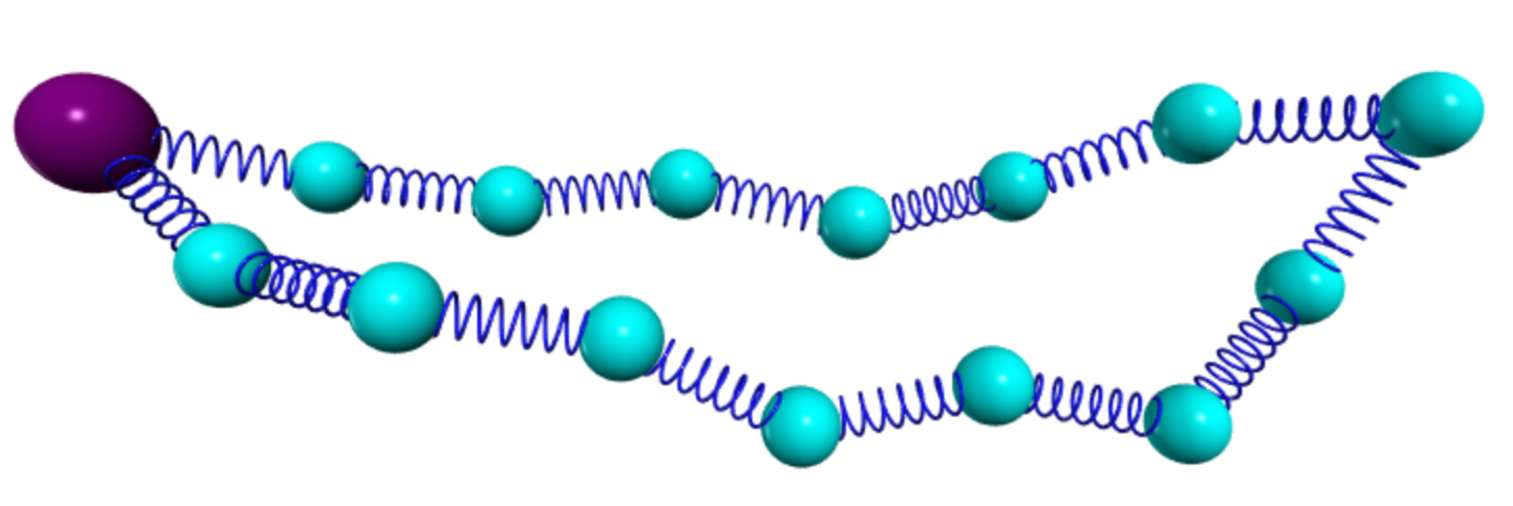
\includegraphics[width=0.8\linewidth]{beadspring}
    \caption{Sketch of the bead-spring loop model. The magenta bead represents the SPB and other cyan beads represent the chromosome segments.}
    \label{fig:beadspring}
\end{figure}

To model the chromosome in fission yeast during nuclear oscillation, we also need a looping structure like the bead-rod model above. The first bead represents the SPB, shown in Fig. \ref{fig:beadspring}. The dynamical equation is similar to the bead-rod model, can be written as following
\begin{equation}
    \label{eq:beadspringEq}
    \xi \frac{d \mathbf{r}_i}{d t} = \mathbf{F}_i^{u} + \mathbf{F}_i^{spring} + \mathbf{F}_i^{e} + \mathbf{F}_i^{b}.
\end{equation}
The notations here are the same as the bead-rod model. In addition, the Brownian force, external force and the potential force are the same as in the bead-rod model. What is different is that the \emph{pseudo} force is not needed and the constraint force is replaced by the spring force $\mathbf{F}_i^{spring}$. Notice that for a bead in the loop, there are two springs connecting to it. Thus
\begin{equation}
    \label{eq:springForce}
    \mathbf{F}_i^{spring} = F_{i+1}^s(Q_{i+1})\mathbf{u}_{i+1} - F_{i}^s(Q_{i})\mathbf{u}_{i},
\end{equation}
here, $F_i^s(Q_i)$ is the tension of the $i^{\rm{th}}$ spring and $Q_i$ is the length of the spring. $\mathbf{u}_i$ is the unit vector for the orientation of the $i^{\rm{th}}$ spring.

There are different types of springs one can use for the model. Here, we will introduce two most commonly used ones and both are used somewhere in the later chapters.

$\bullet$ Hookean spring

Hookean spring is a linear spring, where the tension of spring depends linearly on the length. 
\begin{equation}
    \label{eq:hookeanSpring}
    F^{Hookean} = H (Q-Q_0),
\end{equation}
where $H$ is the Hookean spring constant and $Q_0$ is the natural length of the spring. In practical $Q_0$ is set to $a$, which equals to the length of the bead-rod model. However, sometimes the zero length springs are used. We will point out when needed. 

$\bullet$ Finite Extensible Nonlinear Elastic (FENE) spring

FENE spring is another commonly used spring. The force law of the spring is
\begin{equation}
    \label{eq:feneSpring}
    F^{FENE} = \frac{H Q}{1-(Q/R_0)^2},
\end{equation}
here $R_0$ is the maximal length of the spring. As we can see in Eq. \eqref{eq:feneSpring}, $F^{FENE}\rightarrow\infty$ when $Q\rightarrow R_0$. 


In this section, we specify the dynamics and interaction details of our model for the meiotic chromosomes. The governing equations for the monomers are given. However, we have not talked about the special bead representing the SPB. We will discuss how to pin the SPB in next section.

%********************************** %Second Section  *************************************

\section{Brownian Dynamics simulations}
\label{sec:brownian_dynamics_simulations}
After introducing the model, in this section, we will illustrate how to simulation the model numerically. Since we plan to do most of the theoretical analysis in the later chapters where the simulation results are used for the benchmark, it is convenient that we show the methods of simulation before that. 

Brownian Dynamics (BD) simulation is a kind of Molecule Dynamics (MD) simulation technique. The governing equation of each monomer or particle is integrated to get the trajectories. And physical quantities are measured by ensemble average over trajectories of thousands of monomers. In our situation, the governing equations are Eq. \eqref{eq:beadrodEq} or Eq. \eqref{eq:beadspringEq}. Our interested quantities are something like the average space distance between two beads, the typical size of the polymer and the characteristic time scale of the system dynamics. These are all tractable by BD simulations. 

In the following subsections, we will introduce the algorithms used to do the bead-rod and bead-spring simulation separately. The simulation code is implemented in C++2011. Most the simulation are computed in our clusters with $X86$ architecture.

\subsection{BD simulation of the bead-rod model}
\label{sub:bd_of_bead_rod_model}

Essentially, the goal of the simulation is  to solve the first order ordinary stochastic differential equation Eq. \eqref{eq:beadrodEq} numerically. However, the simple integration algorithm such as the Euler algorithm would not work here. This is because of the implicit constraint force $\mathbf{F}_i^{c}$. Here we employ the predictor-corrector algorithm introduced by Liu \cite{Liu1989}. 

To simplify the illustration of the algorithm, we will ignore all complex potential forces and the external force in Eq. \eqref{eq:beadrodEq}, i.e. $\mathbf{F}_i^{u} = \mathbf{F}_i^{e} = \mathbf{0}$. It is easy to add them back after knowing the algorithm. The dynamical equation after simplification looks 
\begin{equation}
    \label{eq:beadrodSimple}
    \frac{d \mathbf{r}_i}{d t} = \frac{1}{\xi}\left(\mathbf{F}_i^{c} + \mathbf{F}_i^{pseudo} + \mathbf{F}_i^{b}\right).
\end{equation}

The predictor-corrector algorithm is a two-step algorithm and can be divided into the prediction step and correction step. Let us discuss in details.

\subsubsection{Prediction step}
In the prediction step, the estimation of next time step bead position is evaluated without considering the constraints
\begin{equation}
    \label{eq:beadrodPredict}
    \mathbf{r}_i^*(t+\Delta t) = \mathbf{r}_i(t) + \frac{1}{\xi}(\mathbf{F}_i^{pseudo} + \mathbf{F}_i^{b})\Delta t.
\end{equation}
In order to do the calculation, we need to evaluate the Brownian force and the \emph{pseudo} force first. Here we will show how to do that one by one.

$\bullet$ Evaluation of the Brownian force $\mathbf{F}_i^{b}$

The Brownian force is mathematically generated by a Wiener process. Numerically, it is evaluated by a Gaussian distributed \emph{pseudo} random number generated by the computer. Eq. \eqref{eq:beadrodPredict} can be written more practically as 
\begin{equation}
    \begin{aligned}
    \label{eq:beadrodBrownianForce}
    \mathbf{r}_i^*(t+\Delta t) & = \mathbf{r}_i(t) + \frac{1}{\xi}\mathbf{F}_i^{pseudo}\Delta t + \sqrt{\frac{2k_B T}{\xi}}~d\mathbf{W}_i  \\
    & = \mathbf{r}_i(t) + \frac{1}{\xi}\mathbf{F}_i^{pseudo}\Delta t + \sqrt{\frac{2k_B T}{\xi} \Delta t}~\mathbf{N}_i (0, 1),
    \end{aligned}
\end{equation}
where $d\mathbf{W}_i$ is a Wiener process and $\mathbf{N}_i(0,1)$ is a multi-dimensional Gaussian random number of mean $0$ and variance $1$.

$\bullet$ Evaluation of the \emph{pseudo} force $\mathbf{F}_i^{pseudo}$

The expression for \emph{pseudo} force is listed as Eq. \eqref{eq:pseudoForce}. However, the evaluation is not easy and also expensive. To do that, let us first discuss the metric tensor $\mathbf{G}$. 
\begin{equation}
    \label{eq:metricTensor}
    {G}_{\alpha\beta} = \sum_i \frac{\partial g^\alpha}{\partial \mathbf{r}_i} \cdot \frac{\partial g^\beta}{\partial \mathbf{r}_i},
\end{equation}
where $g^\alpha$ is the rigid constraint that 
\begin{equation}
    \label{eq:rigidConstraint}
    g^\alpha(\mathbf{r}_1,\mathbf{r}_2,\cdots,\mathbf{r}_{L}) = 0.
\end{equation}
In the case of a bead-rod loop, Eq. \eqref{eq:rodConstraint} is the constraint. And the $L\times L$ metric tensor looks like
\begin{equation}
    \label{eq:metricMatrix}
    \mathbf{G} = 
    \begin{bmatrix}
        d_1 & c_1 & 0   & \cdots  & c_L \\
        c_1 & d_2 & c_2  &  \cdots & 0 \\
        \vdots & \ddots &\ddots &\ddots &\vdots\\
        0 & \cdots & c_{L-2} & d_{L-1} & c_{L-1} \\
        c_L & \cdots & 0 & c_{L-1} & d_{L}
    \end{bmatrix},
\end{equation}
where diagonal elements $d_i = 2$, and the off-diagonal elements 
\begin{equation}
    c_i = -\mathbf{u}_i\cdot\mathbf{u}_{i-1}
\end{equation}
Again here, the periodic index is applied, i.e. $\mathbf{u}_0 = \mathbf{u}_L$. Now, the \emph{pseudo} force can be calculated as 
\begin{equation}
    \begin{aligned}
    \label{eq:pseudoForceEvaluate}
    \mathbf{F}_i^{pseudo} & = - \frac{1}{2} k_B T \frac{\partial \ln(\det\mathbf{G})}{\partial \mathbf{r}_i} \\
    & = - \frac{1}{2} k_B T \sum_{\alpha,\beta}\frac{1}{\det\mathbf{G}}\frac{\partial\det\mathbf{G}}{\partial{G}_{\alpha\beta}}\frac{\partial{G}_{\alpha\beta}}{\partial\mathbf{r}_i} \\
    & = - \frac{1}{2} k_B T \sum_{\alpha,\beta}{G}_{\beta\alpha}^{-1}\frac{\partial{G}_{\alpha\beta}}{\partial\mathbf{r}_i}.
    \end{aligned}
\end{equation}
In order to calculate the \emph{pseudo} force, we need to inverse the matrix $\mathbf{G}$. This operation is very expensive. Fortunately, the symmetric shape of $\mathbf{G}$ in Eq. \eqref{eq:metricMatrix} makes it possible to find an efficient algorithm to do the computation. We employ the algorithm developed by Pasquali and Morse in \cite{Pasquali2002}. They developed this algorithm for BD simulation of a bead-rod chain. We modified it and successfully applied it to our bead-rod ring model. See Appendix X for details.  

Now the prediction of next time step bead position can be calculated straight forward using Eq. \eqref{eq:beadrodBrownianForce}. The evaluation of other types of forces is quite simple if needed. And we are ready to discuss the correction step.

\subsubsection{Correction step}
The correction step utilizes the result of the prediction, and correct it with the constraint force to obtain the real next time step bead position. 
\begin{equation}
    \label{eq:beadrodCorrect}
    \mathbf{r}_i(t+\Delta t) = \mathbf{r}_i^*(t+\Delta t) + \frac{1}{\xi}\mathbf{F}_i^{c}\Delta t.
\end{equation}
And we known that the rigid rod constraints must be satisfied after the correction. Substitute Eq. \eqref{eq:beadrodCorrect} into Eq. \eqref{eq:rodConstraint} and also notice that 
\begin{equation}
    \label{eq:tensionRod}
    \mathbf{F}_i^{c} = \lambda_{i+1}\mathbf{u}_{i+1} - \lambda_{i}\mathbf{u}_{i}
\end{equation}
where $\lambda_i$ is the magnitude of tension on the $i^{\rm{th}}$ rod. Thus we obtain
\begin{equation}
    \begin{aligned}
    \label{eq:rodTensionEq}
    & 2\Delta t\mathbf{b}_i\cdot\left(\lambda_{i-1}\mathbf{u}_{i-1}-2\lambda_i\mathbf{u}_i+\lambda_{i+1}\mathbf{u}_{i+1}\right) \\
    = &\xi\left(a^2 - \mathbf{b}_i\cdot\mathbf{b}_i\right) -\frac{(\Delta t)^2}{\xi}\left(\lambda_{i-1}\mathbf{u}_{i-1}-2\lambda_i\mathbf{u}_i+\lambda_{i+1}\mathbf{u}_{i+1}\right)^2.
    \end{aligned}
\end{equation}
And $\mathbf{b}_i = \mathbf{r}_i^*(t+\Delta t)- \mathbf{r}_{i-1}^*(t+\Delta t)$. This is a set of nonlinear algebra equations. The second term at the right hand side is the nonlinear term. We can see from here, the nonlinear term is small when the time step $\Delta t$ is small enough. Numerically, it is suitable to use the iteration methods such like the Picard's method to solve this set of equations. High order methods like the Newton's method are also applicable but require the calculation of Jacobian matrix every time step. In practical, a small time step is necessary for the convergence of root searching. We use a time step between $10^{-5}-10^{-3}$ depends on different situations. 

Once we solve the tension $\lambda_i$, plug in to Eq. \eqref{eq:tensionRod} and then Eq. \eqref{eq:beadrodCorrect}, the next time step bead position can be calculated straight forward. 

Finally, We want to discuss a little bit about how to pin the first bead of the bead-rod model. One has several possible ways to do this. The first one is to use a very stiff zero-length spring attached it to the first bead and certain point. This method is very easy to implement. However, the use of the pining spring will introduce a high-frequency factor into the polymer dynamics. This is not good when we analysis of the polymer dynamics. And the spring length is not perfectly zero when the polymer is subjected to a strong force field. So we use another method, i.e. pin the first bead use the zero-length rigid rods. In fact, we will need three this kind of ``ghost'' rods in 3D, the orientation of the rods along three axes respectively. This method requires solving the additional constraint forces. And the calculation is more or less the same as we stated here. With this method, the bead can be pinned perfectly and no disturbing factor will be introduced. 

\subsection{BD simulation of the bead-spring model}
\label{sub:bd_of_bead_spring_model}

The BD simulation of the bead-spring model is much simpler than the bead-rod model. There is neither implicit force nor complex forces need to evaluate during every time step. Of course, one can also use an implicit algorithm which allowed the using of a larger time step. However, we will simply use the explicit algorithms since they work pretty well. 

We will introduce here two simple algorithms to simulate the bead-spring ring polymer, i.e. the Euler method and the stochastic Runge-Kutta method.

\subsubsection{Euler method}

Euler method, also called Euler-Maruyama method, is a 
$1/2$ order integration scheme. In principle, the convergence is only guaranteed when $\Delta t \rightarrow 0$. However, it is still widely used because of its simplicity, especially when the variation of the drift and diffusive term in the stochastic differential equation is not too large. The beads connected by Hookean spring is a good example fits this method. 

Using this method, the next time step bead position in our simple example can be calculated as
\begin{equation}
    \label{eq:beadspringEuler}
    \mathbf{r}_i(t+\Delta t) = \mathbf{r}_i(t) + \frac{1}{\xi}\mathbf{F}_i^{det}\Delta t + \sqrt{\frac{2k_B T}{\xi} \Delta t}~\mathbf{N}_i (0, 1),
\end{equation}
where $\mathbf{F}_i^{det}=\mathbf{F}_i^{u}+\mathbf{F}_i^{spring}+\mathbf{F}_i^{e}$ is the total deterministic force. Also notice that, the $\mathbf{F}_i^{spring}$ is evaluated by Eq. \eqref{eq:springForce} and the spring force law Eq. \eqref{eq:hookeanSpring} or Eq. \eqref{eq:feneSpring}.

\subsubsection{Stochastic Runge-Kutta method}
Stochastic Runge-Kutta method is a higher order integration scheme than the Euler method. It was proposed by Honeycutt in \cite{Honeycutt1992a}. In this method, the next time step bead position can be calculated as
\begin{equation}
    \label{eq:beadspringRK}
    \mathbf{r}_i(t+\Delta t) = \mathbf{r}_i(t) + \frac{1}{\xi}(\mathbf{F}_i^{det}+\tilde{\mathbf{F}}_i^{det})\frac{\Delta t}{2} + \sqrt{\frac{2k_B T}{\xi} \Delta t}~\mathbf{N}_i (0, 1),
\end{equation}
where $\mathbf{F}_i^{det}$ and $\tilde{\mathbf{F}}_i^{det}$ are the total deterministic force evaluated using different bead position.
\begin{equation}
    \begin{aligned}
        \mathbf{F}_i^{det} & = \mathbf{F}_i^{det}\left(\mathbf{r}_0(t),\mathbf{r}_1(t),\cdots,\mathbf{r}_{L-1}(t)\right), \\
        \tilde{\mathbf{F}}_i^{det} & = \tilde{\mathbf{F}}_i^{det}\left(\mathbf{r}_0^*,\mathbf{r}_1^*,\cdots,\mathbf{r}_{L-1}^*\right),
    \end{aligned}
\end{equation}
and $\mathbf{r}_i^*$ is the mid-step bead position
\begin{equation}
    \mathbf{r}_i^*  = \mathbf{r}_i(t) + \frac{1}{\xi}\mathbf{F}_i^{det}\Delta t  + \sqrt{\frac{2k_B T}{\xi} \Delta t}~\mathbf{N}_i (0, 1).
\end{equation}

Last but not least, in the simulations, the dynamical equation is nondimensionalized by rescaling the variable in the following way:
\begin{equation}
    \label{eq:dimensionless}
    \mathbf{r}^{\prime}\to \mathbf{r}/a;~t^{\prime}\to t/(\xi a^2/k_BT);~\mathbf{F}^{\prime}\to\mathbf{F}/(k_BT/a).
\end{equation}
After the rescaling, the length unit is set to the size of the rod. The rescaling is helpful to avoid doing calculations with very small or big numbers, which might introduce larger numerical errors. 


%********************************** % Third Section  *************************************
\section{Monte-Carlo simulation of the bead-rod model}
\label{sec:monte_carlo_simulation_of_the_bead_rod_model}

In the previous section, we present the BD simulation technique of the bead-rod and bead-spring polymer loop. As we can see there, the algorithm used to simulate the bead-rod model is actually quite complex and also time-consuming. Sometimes we do not need to do that if we only want to sample the equilibrium properties of the bead-rod system. In this section, we will introduce a Monte-Carlo algorithm that is much faster and efficient to obtain the equilibrium statistics of the bead-rod loop model. 

Monte-Carlo technique has used to simulate the polymer system for a long time \cite{Binder1995}. However, there are some special factors one need to take into account for our pinned polymer loop model. Basically, one has to preserve the loop structure and keep the rod length fixed when trying to do a Monte-Carlo flip. According to this, we propose the following main steps of our Monte-Carlo algorithm. 

$\bullet$ Step I: prepare an initial configuration and compute the energy of this configuration. The way of calculating system energy depends on the setting of the model, whether the excluded volume effect or other interactions are taken into account or not. For example, the energy of a pinned bead-rod loop in a constant external force field can be written as
\begin{equation}
    \label{eq:mcEnergy}
    E = U - \sum_{i=1}^L\mathbf{F}^{e} \cdot \mathbf{r}_i
\end{equation}
where $U$ is other kind of interaction energy. In the simplest case, we will assume $U$ is independent of the configurations. To compare with the later evaluation, we denote the energy calculated here $E_{old}$.

$\bullet$ Step II: randomly choice two beads in the polymer loop, use the connecting line between the two beads as a rotation axis.
\begin{figure}[htpb]
    \centering
    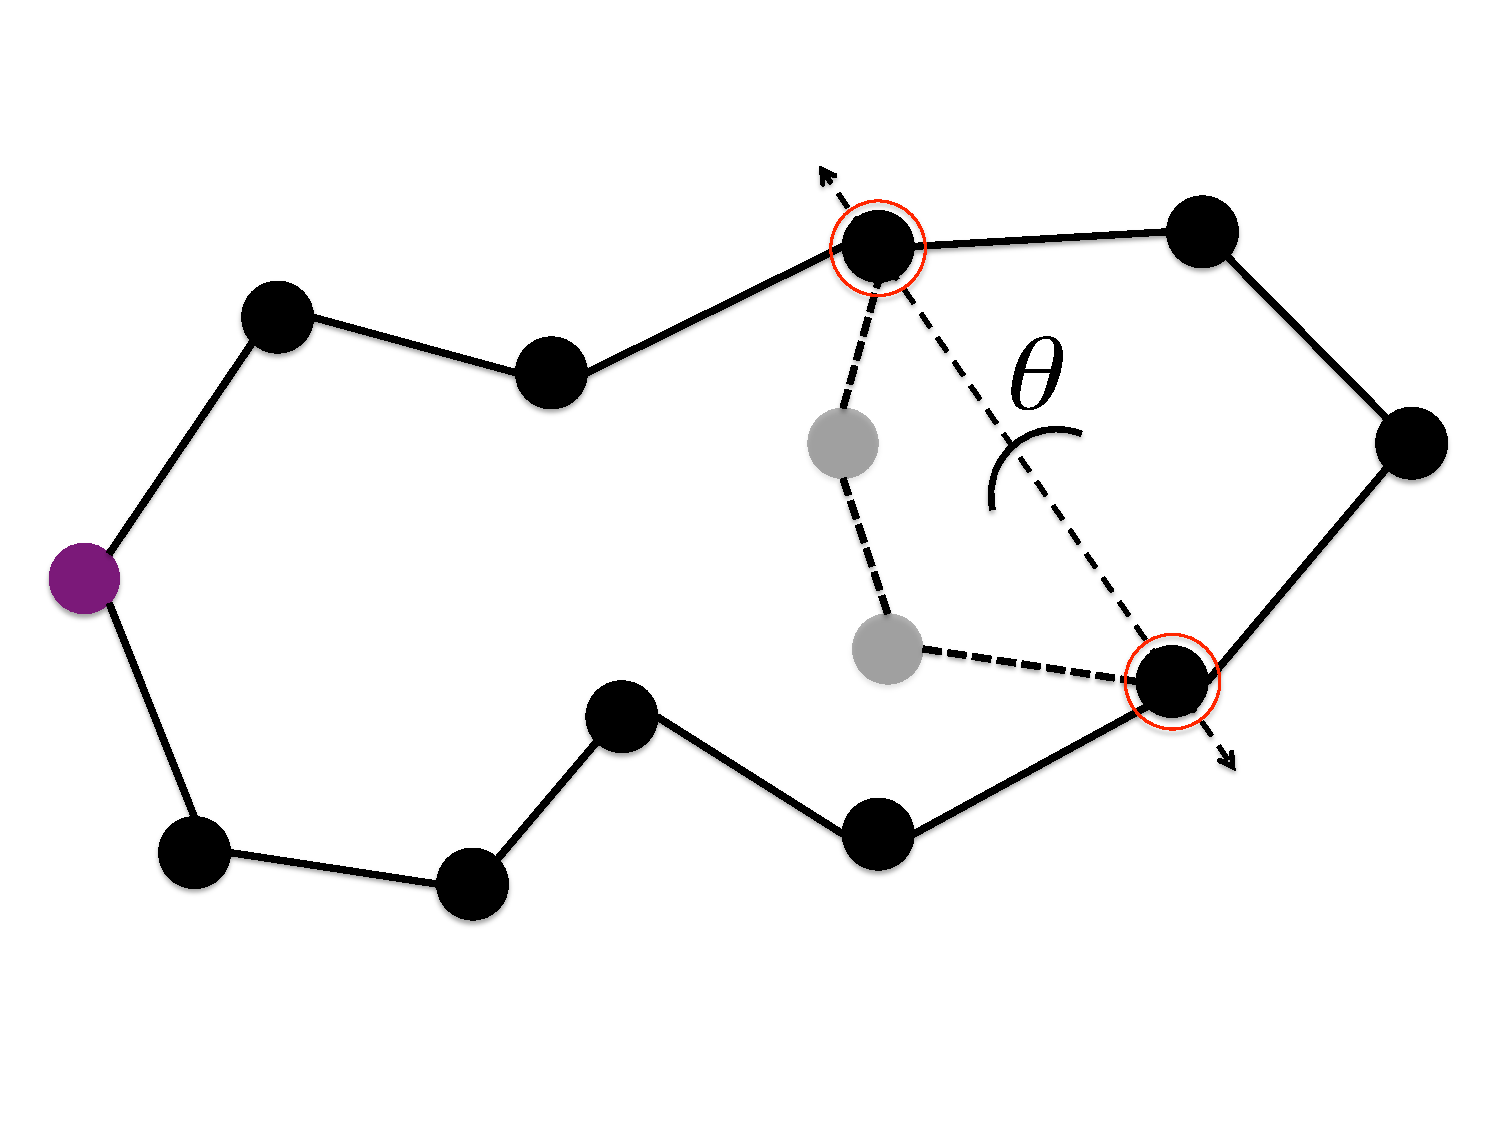
\includegraphics[width=0.8\linewidth]{rotation}
    \caption{Illustration of the Monte-Carlo configuration flip. }
    \label{fig:rotation}
\end{figure}

$\bullet$ Step III: choose the unpinned side of the polymer, and rotate this part of the polymer by a random angle $\theta\in[-\phi, \phi]$. $\phi$ is a parameter between $[0,\pi]$ and can be tuned to improve the efficiency of the algorithm. See in Fig. \ref{fig:rotation}. If the pinned bead is selected, then randomly choose a side of the polymer to do the rotation. 

$\bullet$ Step IV: calculated the energy of the configuration after rotation in the same way of $E_{old}$. Let us denote the new energy as $E_{new}$.

$\bullet$ Step V: the new configuration is accepted with probability  
\begin{equation}
    \label{eq:mcProbability}
    p = \min\left\{1, \exp\left(-\frac{\Delta E}{k_BT}\right)\right\},
\end{equation}
where $\Delta E = E_{new} - E_{old}$. If not accepted, then the polymer returns to the old configuration, and try again with new random number. An efficient sampling algorithm can be tuned by parameter $\phi$ so that the accept probability is around $0.5$.

$\bullet$ Step VI: go back to step I and loop again and again to get enough independent samples. Physical quantities such like the statistical distance between two beads can be calculated by averaging over these samples.

The Monte-Carlo method introduced in this section is efficient and fast, we will use it to calculate most of the equilibrium quantities in next chapter. On the other hand, the Monte-Carlo results also work as a benchmark of the BD simulation and vice-versa. 


%********************************** % Fourth Section  *************************************

\section{Summary}
\label{sec:summary_chap2}

In this chapter, we elaborated the details of our pulled polymer model for the chromosomes in meiotic fission yeast. We have shown that the pulled polymer loop is equivalent to the pinned polymer loop in external force field after a coordinate transform. The concrete bead-rod and bead-spring polymer loop models are discussed. And the BD simulation technique is discussed in details. A Monte-Carlo algorithm is introduced to calculate the equilibrium statistics of the bead-rod system and overcomes the disadvantages of heavy computation for the BD simulation.

The content of this chapter will be very useful in our later chapters. And we try to keep it concise, many related interesting models or methods are not mentioned here. Only those that will use in this thesis are discussed. Interested readers can refer to the cited references.

In next chapter, we will start to discuss the theory of equilibrium statistics of our polymer model and use the theory to explain the chromosome alignment in fission yeast. 

\chapter{Equilibrium Statistics of the Forced Pinned Polymer Loop}
\graphicspath{{Chapter3/Figs/}}

In previous chapter, we introduced the details of our polymer loop model for chromosomes and the simulation techniques. In this chapter, we will investigate the equilibrium statistics of the model and use the results to understand the chromosome alignment in fission yeast. 

In order to tract the model analytically, we will neglect the complex interactions such as bending energy, excluded volume effect and hydrodynamical perturbations. In another word, our model is the simplest freely-jointed polymer loop model. The transferred coordinate is utilized so that the first bead representing SPB is pinned. And an external force field will be applied. 

We will start by introducing the setting of the model in the first section. The equilibrium statistics of 1D and 3D are discussed separately in section two and three. In the fourth section, we discuss of shape of steady pinned polymer loop in external force field. We want to mention here that the work of first three sections were done by close cooperation with Yen Ting Lin. Most of the theory was developed by him and I contribute to all the simulations. 


%********************************** %First Section  **************************************
\section{Pinned polymer loop in a constant force field}
\label{sec:pinned_polymer_loop}
\begin{figure}[htpb]
    \centering
    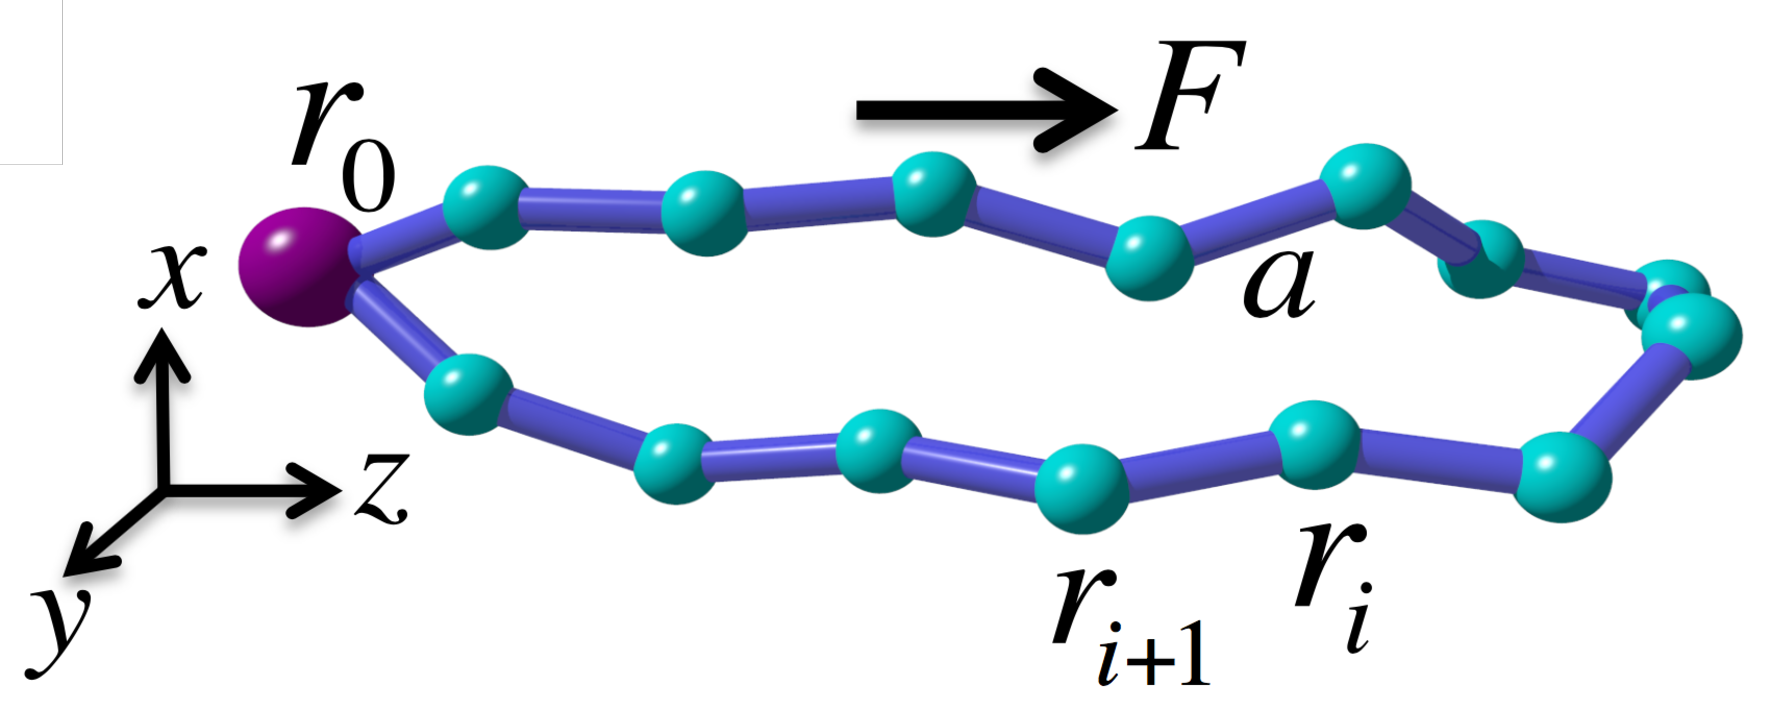
\includegraphics[width=0.7\linewidth]{beadrod}
    \caption{Sketch for the pinned bead-rod loop and notations. }
    \label{fig:beadrod}
\end{figure}

As mentioned in section~\ref{sec:polymer_model_and_dna}, the chromosomes of fission yeast can be considered as pulled polymers with constant velocity during the period of moving towards to one direction. In this case, it is appropriate to discuss the equilibrium statistics as the relaxation time scale is much smaller than the oscillation time scale. Using the coordinate transformation introduced in the section~\ref{sec:stochastic_models_of_polymer_loops}, the pulled polymer loop model can be transferred to pinned polymer loops in constant external force field. We will discuss the equilibrium statistics of the pinned polymer loops in an external force field in this chapter.

Let us first clarify some notations before seeking for the solution. There are $L$ beads (including the SPB) in the loop and the SPB is denoted by $\mathbf{r}_0$ or $\mathbf{r}_L$ in periodic indexing. Without loss of generality, we assume it is pinned to the origin point, i.e. $\mathbf{r}_0 = \mathbf{r}_L = \mathbf{0}$. The length of each rod is $a$. And the constant external force field denotes by $\mathbf{F}$ is in the $z$ direction. The potential energy of the pinned polymer loop can be written as:
\begin{equation}
    \label{eq:energyBeadrod}
    E = E_0 - a\sum_{i=1}^{L} \mathbf{F}\cdot\mathbf{r}_i
\end{equation}
where $E_0$ is assumed to be a constant that denotes configuration independent energy. It is not important for the study of equilibrium statistics, we keep it here just for completeness. The orientation of the $j^{\rm{th}}$ rod is denoted by $\mathbf{u}_j = (\mathbf{r}_{j}-\mathbf{r}_{j-1})/a$. So the $i^{\rm{th}}$ bead position can be written as:
\begin{equation}
    \label{eq:beadposRodsum}
    \mathbf{r}_i = a \sum_{j=1}^{i} {u}_j.
\end{equation}
Plug it into Eq.~\eqref{eq:energyBeadrod}, we arrive at
\begin{equation}
    \label{eq:energyRodsum}
    E = E_0-a\sum_{i=1}^{L}\sum_{j=1}^{i}\mathbf{F}\cdot\mathbf{u}_j.
\end{equation}
Notice that the looping condition indicates
\begin{equation}
    \label{eq:loopCondition}
    \sum_{j=1}^{L} \mathbf{u}_j = 0.
\end{equation}

In the following two sections, we will solve the equilibrium statistics in 1D first and extend the theory to 3D.


%********************************** %Second Section  *************************************
\section{Pinned Polymer Loop in 1D}
\label{sec:pinned_polymer_loop_in_1d}

As the same strategy to study many problems in physics, let us start to solve the equilibrium statistics from the simplest 1D case. The one dimensional polymer is possible because we neglect the exclusion volume effect so that the beads and rods are free to overlap. It is a simple idealized model. We will show in the following that an elegant mapping for the one dimensional pinned polymer loop to a famous classical physical model can be found. 

\subsection{Mapping to a particle system on 1D lattice}
\label{sub:mapping_to_a_particle_system_on_1d_lattice}

The pinned polymer in 1D is very simple. The configuration of the polymer can be specified by the orientation of the rods. In 1D, there are only two possible orientations for all rods, i.e. along the axis or against the axis. 

Let us denote the $j^{\rm{th}}$ rod orientation by $u_j\in\{-1, +1\}$, where $u_j = +1$ means the rod orientates along the axis and $u_j = -1$ means the rod orientates against the axis. Again the $i^{\rm{th}}$ bead position in 1D is $z_i = a\sum_{j=1}^{i}u_j$. Now let us introduce a shifted and rescaled variable 
\begin{equation}
    \label{eq:variableu2n}
    n_j = (u_j + 1)/2. 
\end{equation}
We can easily find that $n_j\in\{0,1\}$. The configuration of the 1D polymer can be denoted by $\{n_1, n_2, \cdots, n_L\}$. Since $n_j$ is a binary variable, we can interpret $n_j = 1$ as a lattice site occupied by a particle, and $n_j = 0$ as an empty lattice site. In this way, we find a one-to-one mapping from the configuration of polymers to particles on lattice sites. See in Fig. \ref{fig:mapping}. The number of rods equals to the number of lattice sites. Without loss of generality, we have shown in the figure the right-orientated rod corresponds to an occupied site, and the left-oriented rod corresponds to an empty site.

\begin{figure}[htpb]
    \centering
    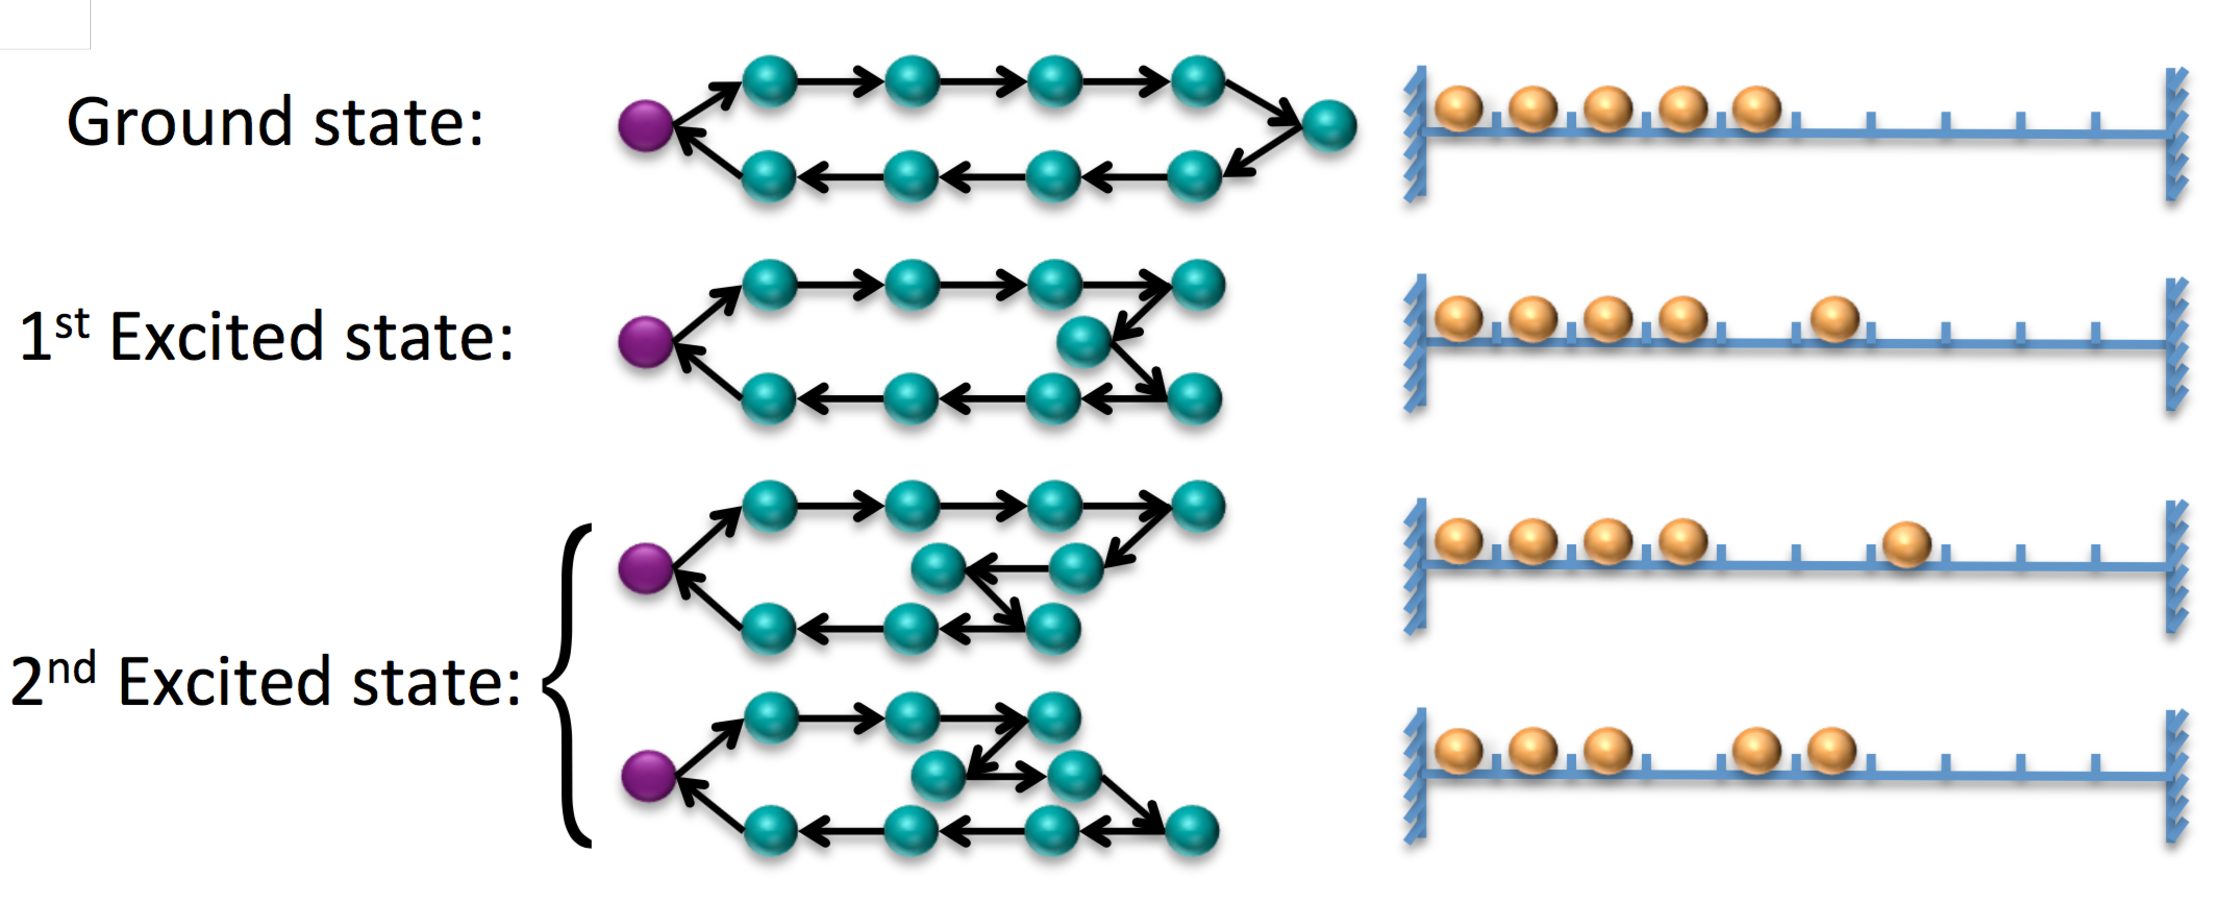
\includegraphics[width=0.9\linewidth]{mapping}
    \caption{Illustration for the mapping from 1D pinned polymer loop to Fermionic particles on 1D lattice sites. }
    \label{fig:mapping}
\end{figure}

Here are some remarks for the mapping:

$\bullet$ The mapped particles are exclusive to each other. It is not possible for one lattice occupied by more than one particles. In another word, these particles are Fermions. This is because the system is a two state system, there is no correspondent polymer state for a site occupied by more than one particle.

$\bullet$ According to the looping condition Eq. \eqref{eq:loopCondition}, the total number of rods pointing to the right must be exact $L/2$. Correspondingly, the total number of particles also must be exact $L/2$, i.e.
\begin{equation}
    \label{eq:loopConditionParticle}
    \sum_{j=1}^{L}{n_j} = \frac{L}{2}.
\end{equation}
Furthermore, the number of particles must be conserved during the change of configurations.

$\bullet$ The dynamics of 1D polymer can be mapped to the particle hopping process on the 1D lattice. This part will be discussed in next chapter.

$\bullet$ The mapping is essentially from a two state system to a two state system. One can also interpret the two state as spin up and spin down or any other two state systems. We use the particle-lattice interpretation because it is familiar and intuitive to most people. 

Now let us discuss the energy of the system. Rewrite Eq. \eqref{eq:energyRodsum} in 1D we get
\begin{equation}
    \label{eq:energyRodsum1D}
    E = E_0 - Fa \sum_{i=1}^L\sum_{j=1}^i u_j.
\end{equation}
Exchange the summation order in Eq. \eqref{eq:energyRodsum1D} and utilizing the loop condition $\sum_{j=1}^L u_j = 0$ we obtain
\begin{equation}
    \label{eq:energy1D}
    E = E_0 + Fa \sum_{j=1}^L j u_j.
\end{equation}
Let us look at the energy from the particle-lattice picture. Substitute Eq. \eqref{eq:variableu2n} into Eq. \eqref{eq:energy1D}, we arrive at
\begin{equation}
    \label{eq:energy1DRewrite}
    E = \tilde{E}_0+\Delta E\sum_{j=1}^{L} j n_j 
\end{equation}
where $\Delta E = 2Fa$ and $\tilde{E}_0 = E_0 - L(L+1)\Delta E/4$ is the unimportant energy offset. Let us ignore the offset in our discussion. Eq. \eqref{eq:energy1DRewrite} can be reinterpret as the summation energy of $L$ lattice sites. When $n_j = 1$ (occupied site), we gain a energy of $j\Delta E$ and zero otherwise. One can clearly see that Eq. \eqref{eq:energy1DRewrite} is the energy of a system of $L/2$ fermions distributed over $L$ equidistant energy levels $\Delta E, 2\Delta E, \cdots, L\Delta E$.
The lowest energy (ground state) corresponds to the configuration that the left half of lattice sites are fully filled by particles. And the corresponding polymer picture is the fulled stretched configuration. The correspondence of the $1^{\rm{st}}$ and the $2^{\rm{nd}}$ excited states also can be imagined, which is shown in Fig. \ref{fig:mapping}. 

The mapping from the polymer to the particle-lattice picture is very useful for searching the solution of equilibrium statistics. In the following subsections, we will solve the 1D statistics using two different methods. The first one based on the grand canonical ensemble is an approximate solution with a simpler formulism, while the second one is the exact solution based on the canonical ensemble but a more complex formulism. We will calculate the mean position of beads and their variance. Because these are what we interested, the biological interactions can only happen when two segments are closer enough. 

\subsection{Grand canonical ensemble solution}
\label{sub:grand_canonical_ensemble_solution}
We have mentioned in the previous subsection that the particle number is conserved to $L/2$ in the mapped particle-lattice picture. So in principle, the system is a canonical ensemble system. However, let us first release this constraint by allowing the particles exchange with the reservoir at both sides of the lattice. Thus the grand canonical ensemble can be applied. After that, we can reimpose the constraint using the Brownian bridge technique. We can obtain very accurate mean bead position and its variance use this method. Given that the formulation of this method is simple, we are quite satisfied with the results. Let us now illustrate the method in details.

\subsubsection{The Fermi-Dirac statistics}
\label{ssub:The Fermi-Dirac Statistics}

As we have mentioned above, the particles on the lattice are Fermions. One wonderful thing of the grand canonical ensemble is the particles can be assumed to be mutually independent. So that we can directly use the famous \emph{Fermi-Dirac} distribution. That is to say the probability of a lattice site is occupied can be written as
\begin{equation}
    \label{eq:fermiDirac}
    \mathbb{P}\{n_j=1\} = \frac{1}{1+\exp\left[\frac{\Delta E (j - \mu)}{k_B T}\right]},
\end{equation}
where $\mu$ is the chemical potential $\mu = (L+1)/2$ obtained from the requirement that on average there are $L/2$ particles in the system. And accordingly, the probability that a lattice site is empty writes
\begin{equation}
    \label{eq:probEmpty}
    \mathbb{P}\{n_j=0\} = 1 - \mathbb{P}\{n_j=1\}.
\end{equation}
Let us define a dimensionless quantity which we call it \emph{dimensionless temperature}:
\begin{equation}
    \label{eq:dimensionlessT}
    \tilde{T} = \frac{k_B T }{\Delta E} = \frac{k_B T}{2Fa}
\end{equation}
Now we can see in Fig. \ref{fig:fermiDirac} for an illustration of the \emph{Fermi-Dirac} distribution of different $\tilde{T}$. When $\tilde{T}$ is small, namely the external force is large, the distribution shows a strong bias. The left half sites are more likely to be occupied and the right half sites are more likely to be empty. In the polymer picture, this means the orientation of the first half rods is biased in the direction of force, whereas the second half of rods are more probable to point against the force field. Physically, it is easy to understand because the pinned polymer in strong force field is almost stretched.

\begin{figure}[htpb]
    \centering
    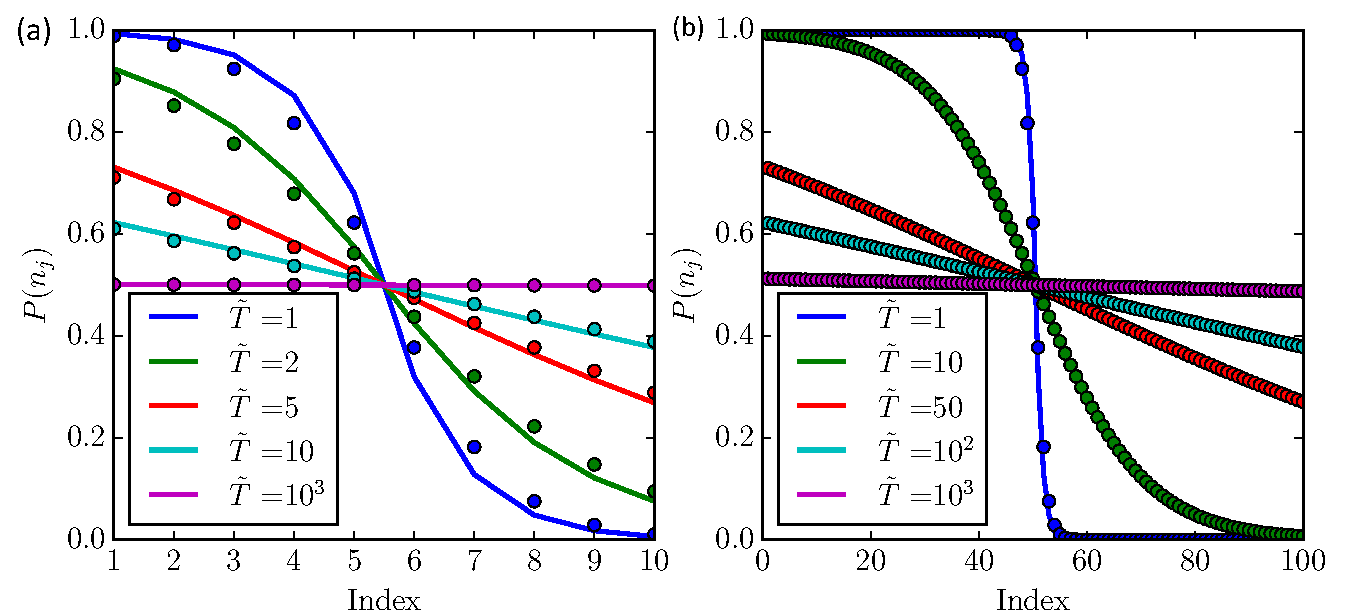
\includegraphics[width=1.0\linewidth]{fermiDirac}
    \caption{Fermi-Dirac distribution compared with the exact solution from the number partition theory. Solid lines are the exact solution while the dots are Fermi-Dirac approximations. Different dimensionless temperature is indicated by different colors as shown in the legend. (a) $L=10$, (b) $L=100$. }
    \label{fig:fermiDirac}
\end{figure}

With Eq. \eqref{eq:fermiDirac}, the mean and variance of random variable $n_j$ can be calculated straightforwardly:
\begin{subequations}
    \begin{align}
        \label{eq:nmean}
        \left<n_j\right> & = \mathbb{P}\left\{n_j=1\right\},\\
        \label{eq:nvar}
        \text{var}\left[n_j\right] & = \mathbb{P}\left\{n_j=1\right\} \cdot \mathbb{P}\left\{ n_j=0\right\} 
        - \left<n_j\right>^2.
    \end{align}
\end{subequations}
On the other hand, from Eq. \eqref{eq:beadposRodsum} and Eq. \eqref{eq:variableu2n} we can calculate the position of bead as
\begin{equation}
    \label{eq:beadpos1D}
    z_i = a\left(2\sum_{j=1}^i n_j - i\right).
\end{equation}
If we assume $n_1, n_2, \cdots, n_L$ are all mutually independent, then the mean and variance of bead position can simply calculated as
\begin{subequations}
    \label{eq:meanVarPos1D}
    \begin{align}
    \label{eq:meanPos1D}
        \left<z_j\right> & = a \left(2\sum_{j=1}^i \left<n_j\right> - i\right),\\
    \label{eq:varPos1D}
        \text{var}\left[z_j\right] & = 4a^2\sum_{j=1}^i\text{var}\left[n_j\right]
    \end{align}
\end{subequations}
The results of the above equations can be compared to the Monte-Carlo simulation (see Appendix \ref{append:mc1D} for details). 
We found that the formula for mean bead position works perfect. However, the formula for variance does not work so good. Notice that Eq. \eqref{eq:varPos1D} is monotonically increasing with the index $i$. We can take the simple symmetric argument that the $\text{var}\left[z_i\right] = \text{var}\left[z_{L-i}\right]$. The result after that still can not match with the simulations. See in Fig. \ref{fig:meanVarAdd1D}.

\begin{figure}[htpb]
    \centering
    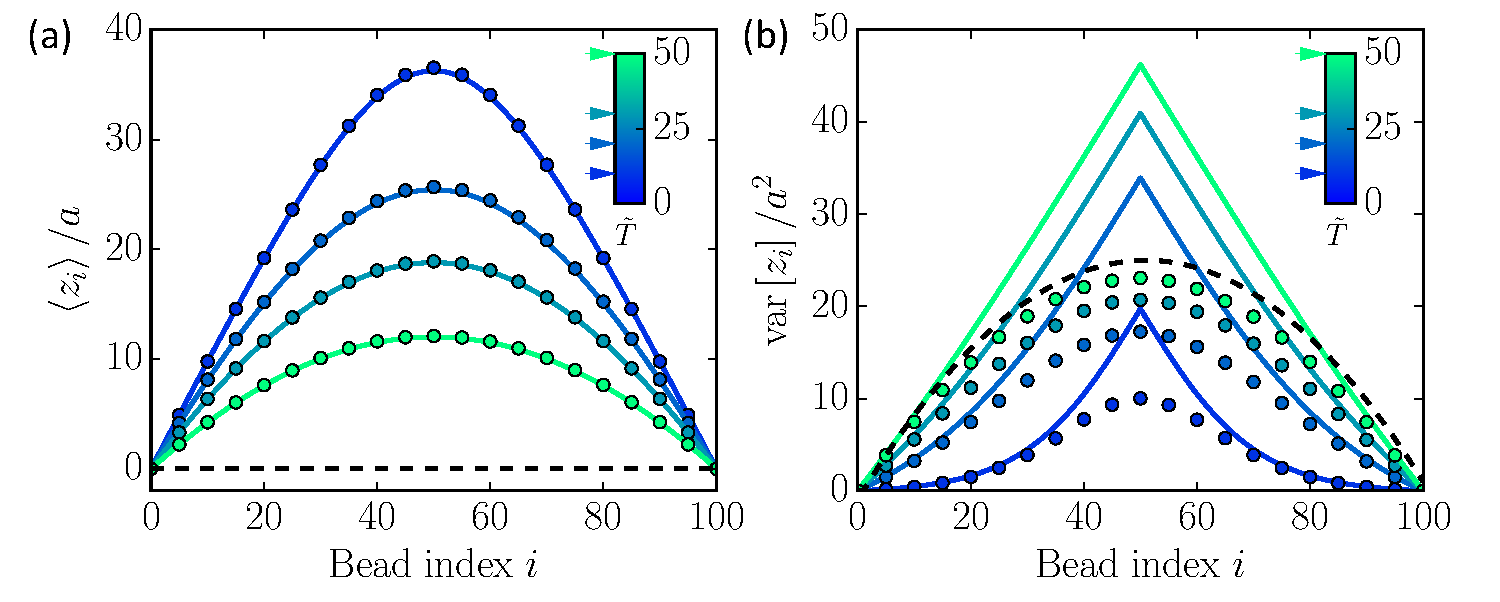
\includegraphics[width=1.0\linewidth]{meanVarAdd1D}
    \caption{Mean and variance of the 1D pinned polymer bead positions. MC simulation results (dots) are compared with theoretical results (solid lines) Eq. \ref{eq:meanVarPos1D}. The length of the polymer loop $L=10$. The black dash line indicates the case $\tilde{T}\rightarrow\infty$, i.e. no external force field. }
    \label{fig:meanVarAdd1D}
\end{figure}

The reason for this mismatch is simple, the particles are not exactly independent and the loop condition is only fulfilled on average by choosing the chemical potential $\mu=(L+1)/2$ in Eq. \eqref{eq:fermiDirac}. In the following part, we will show how to solve this problem use the Brownian bridge technique. 

\subsubsection{The Brownian bridge condition}
\label{ssub:The Brownian Bridge Condition}
Let us consider the polymer loop as a random walk that returns to the origin point after $L$ steps. This sort of random walk process is called the Brownian bridge \cite{Feller2008,Athreya2006}. So each rod represents a random walk step. The segment connecting the $k^{\rm{th}}$ and the $l^{\rm{th}}$ bead corresponds to the propagator $\rho(z_l = z | z_k=0)$. According to the Lindeberg-Feller central limit theorem \cite{Feller2008}, this propagator is Gaussian with the mean and variance equal to the sum of the mean and variance of all individual steps from $k$ to $l$.

As we said above, the grand canonical ensemble only ensures the loop condition on average. To solve the problem, we now impose the Brownian bridge condition so that every single trajectory fulfills the loop condition. The Brownian bridge can be formulated as following:
\begin{equation}
    \label{eq:brownianBridge}
    \rho^L(z_i=z) = \frac{\rho(z_i=z|z_0=0)\rho(z_{L-i}=z|z_L=0)}{\rho(z_L=0|z_0=0)},
\end{equation}
where $\rho(z_i=z)$ is the probability density function of finding the $i^{\rm{th}}$ bead at position $z$, $\rho(z_k=z|z_j=0)$ are the propagators. Eq. \eqref{eq:brownianforce} means that the probability density equals two pieces of random walk trajectory of length $i$ and $L-i$ meet at position $z$ on the condition that they are belong to the same loop. 
\begin{figure}[htpb]
    \centering
    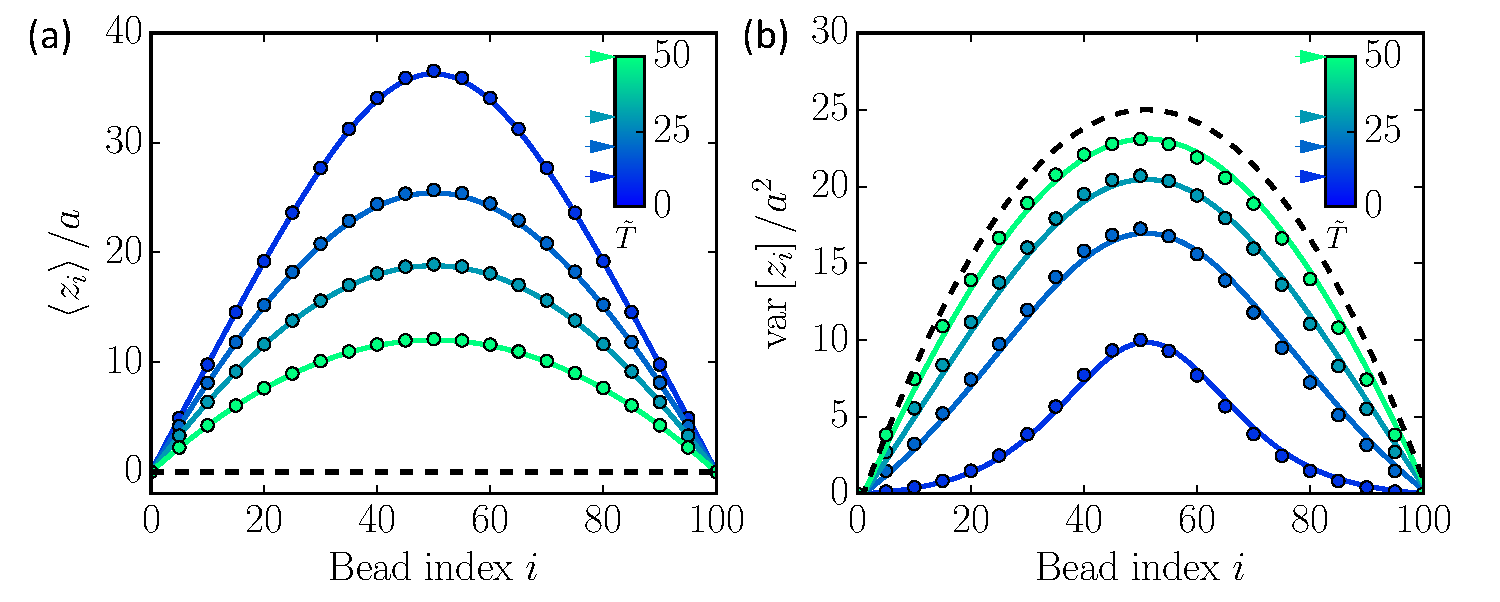
\includegraphics[width=1.0\linewidth]{meanVar1D}
    \caption{Mean and variance of the 1D pinned polymer bead positions. MC simulation results (dots) are compared with theoretical results (solid lines) Eq. \ref{eq:meanVarPos1DExpression}. The length of the polymer loop $L=10$. The black dash line indicates the case $\tilde{T}\rightarrow\infty$, i.e. no external force field. }
    \label{fig:meanVar1D}
\end{figure}

Notice that the propagators are Gaussian with the variance added up by the variance of individual steps, i.e Eq. \eqref{eq:varPos1D}. So that $\rho^L(z_i = z)$ is also Gaussian. Its variance is given by
\begin{equation}
    \label{eq:varBrownianBridge}
    \text{var}\left[z_i\right] = 4a^2\frac{\sum_{j=0}^{i}\text{var}\left[n_j\right]\sum_{j=L-i}^{L}\text{var}\left[n_j\right]}{\sum_{j=0}^{L}\text{var}\left[n_j\right]}.
\end{equation}
Plug in Eq. \eqref{eq:nvar} and Eq. \eqref{eq:varPos1D} we can obtain the variance of bead position in the loop. For $\tilde{T}\gg 1$, we can obtain the close form expressions for mean and variance of bead position by converting the summation to integral
\begin{subequations}
    \label{eq:meanVarPos1DExpression}
    \begin{align}
        \left< z_i \right> & = 2 a \tilde{T} \ln\left[ \frac{1+\exp\left(\frac{L}{2\tilde{T}}\right)}{\exp\left(\frac{i}{2\tilde{T}}\right) + \exp\left(\frac{L-i}{2\tilde{T}}\right)} \right] \\
        \text{var}\left[z_i\right] & = 2 a^2 \tilde{T} \frac{ \sinh\left( \frac{L-i}{2\tilde{T}}\right) \sinh\left( \frac{i}{2\tilde{T}}\right)} {\sinh\left( \frac{L}{2\tilde{T}}\right) \cosh^2\left( \frac{L-2i}{4\tilde{T}}\right)}
    \end{align}
\end{subequations}
We can see from the above formulas that the $z_i-z_{L-i}$ symmetry is satisfied. And a strong external force field leads to a stretched configuration and a small fluctuation of bead position. This result is compared with the Monte-Carlo simulations, see in Fig. \ref{fig:meanVar1D}.

In this subsection, we solved the mean and variance of bead position for 1D pinned polymer loop in an external force field. The strategy is using the \emph{Fermi-Dirac} statistics and re-enforce the loop condition by the Brownian bridge technique. Excellent results verified by the Monte-Carlo simulation are obtained. However, we have to say, this is just an approximate method. In the next subsection, we will use the canonical ensemble to obtain the exact solution. 

\subsection{Canonical ensemble solution}
\label{sub:canonical_ensemble_solution}
In the particle-lattice picture, the system is actually a canonical ensemble system because of the conservation of particle number. In this section, we will calculate the exact partition function using this ensemble. More interestingly, we will show the calculation can be recoded to a number partition problem. Exact results are obtained and compared with the results from the approximate approach above.

\subsubsection{The number partition theory}
\label{ssub:The Number Partition Theory}
Before the calculation of exact partition function, let us discuss an interesting number partition problem that share a lot of similarities with the former. 

Consider a non-negative integer number $K$, which can be expressed into the summation of $N$ non-negative integers:
\begin{equation}
    K = \sum_{j=1}^N k_j
\end{equation}
However, there is a constraint on the summation components $0 \leqslant k_1 \leqslant k_2 \cdots \leqslant k_N \leqslant M$. This kind of problem can be best visualized by what called Young diagram \cite{Andrews1998}, shown in Fig. \ref{fig:young}.
\begin{figure}[htpb]
    \centering
    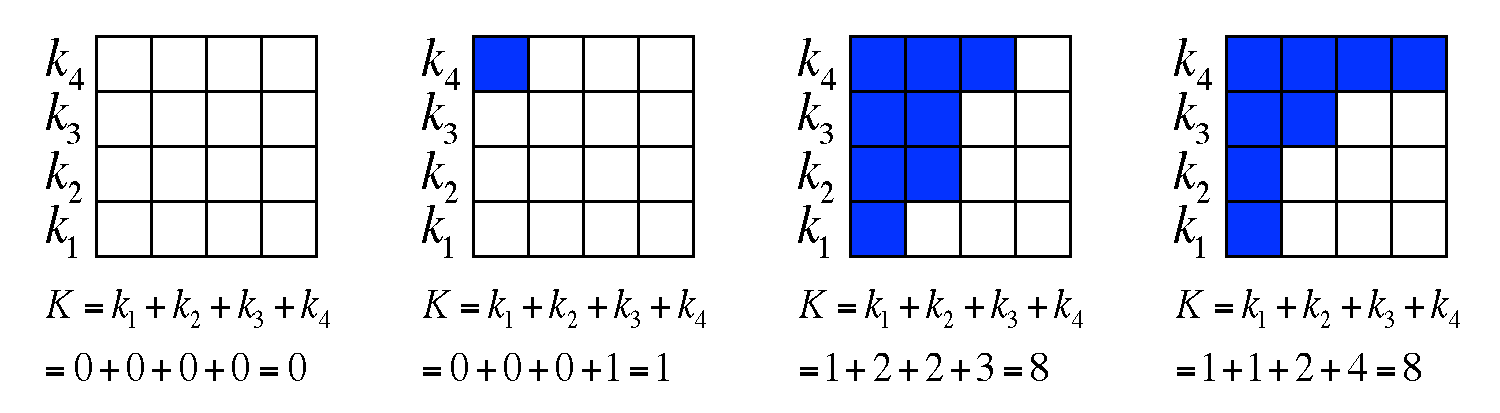
\includegraphics[width=1.0\linewidth]{young}
    \caption{Some examples of the Young diagram.}
    \label{fig:young}
\end{figure}
In the Young diagram, each row represents a integer number. The number of blue boxes means the value of the $j^{\rm{th}}$ integer. Starting from the bottom, because of the constraint, the diagram is non-decreasing. 

The question is, given a certain integer $K$, how many different ways are there to partition it into $N$ non-decreasing pieces $\{k_1, k_2, \cdots, k_N\}$. For the simple cases, one can tell the answer immediately. For examples, in the first two examples of Fig. \ref{fig:young}, we illustrate that there are only one way to partition integer $0$ or $1$ into $4$ non-decreasing integers. However, this question in the general case is not intuitive. Fortunately, this problem is well studied by mathematicians. Let $g(M, N; K)$ denote the number of partitions of $K$ with at most $N$ parts, each of size at most $M$. Equivalently, these are the partitions whose Young diagram fits inside an $N \times M$ rectangle. Then we have the following generating function:
\begin{equation}
    \label{eq:generatingDegeneracy}
    \Phi(q):=\sum_{K=0}^{MN} g(M, N; K) q^K = \binom{M+N}{N}_q
\end{equation}
where $q$ is an auxiliary number, and the notation at the right hand side of Eq. \eqref{eq:generatingDegeneracy} is called $q$ binomial coefficient or Gaussian binomial coefficient. It is defined as 
\begin{equation}
    \label{eq:qBinomial}
    \binom{L}{N}_q := \frac{[L]_q!}{[L-N]_q![N]_q!},
\end{equation}
and $[N]_q := 1 + q + q^2 + \cdots + q^{N-1}$ is called a $q$ number \cite{Andrews1998}.


\subsubsection{Exact partition function}
\label{ssub:Exact Partition Function}
Now, let us start to calculate the partition function of our pinned polymer in the particle-lattice picture. The partition function of a canonical ensemble system with discrete energy can be written as:
\begin{equation}
    \label{eq:partitionFuncCanonical}
    \mathcal{Z}\left(T\right) = \sum_{E}g(E)\exp \left(-\frac{E}{k_B T}\right),
\end{equation}
where $g(E)$ is the degeneracy of the microscopic states which have the same energy $E$. Once $g(E)$ is known, the partition function can be calculated straightforwardly.

Let us take a look at the energy of the system, i.e. Eq. \eqref{eq:energy1DRewrite}. It is represented in the way of rod orientation $u_j$ or occupation variable $n_j$. Here, we are going to use another way to represent the energy. In the particle-lattice picture, the system consists $N:=L/2$ particles. So the energy can be rewritten as:
\begin{equation}
    E = \tilde{E}_0 + \sum_{j=1}^N E_j,
\end{equation}
where $E_j$ is the energy of the $j^{\rm{th}}$ particle in the external force field. Again, $\tilde{E}_0$ is an unimportant constant energy offset. Denote the position of the $j^{\rm{th}}$ particle as $x_j$, which is an integer $x_j\in[1, L]$. Then we can write $E_j = x_j \Delta E$. 
Also notice that, because of the exclusive condition, the sample space of the particle system is constrained in $\Omega = \{\mathbf{x}| 1\leqslant x_1<x_2<\cdots<x_N\leqslant L\}$.

Let us do a shift for the particle position by defining
\begin{equation}
    k_j := x_j - j.
\end{equation}
Notice now the constraint on $x_j$ is transferred to $0 \leqslant k_1 \leqslant k_2 \cdots \leqslant k_N \leqslant N$. And the energy of the system can be rewritten as:
\begin{equation}
    E = \hat{E}_0 + \Delta E \sum_{j=1}^N k_j = \hat{E}_0 + K \Delta E,
\end{equation}
Again $\hat{E}_0$ here is an unimportant constant energy offset, $\hat{E}_0 = \tilde{E}_0+N(N+1)/2$. 
It is not difficult to find the range of the energy is $\hat{E}_0, \hat{E}_0 + \Delta E, \cdots, \hat{E}+N^2\Delta E$. 

Now we are closer to the number partition problem. Notice that $K=\sum_{j=1}^{N}k_j$ and we have the same type of constraint as in the number partition problem. In addition, because the mapping from integer $K$ to energy $E$ is one-to-one. So the degeneracy function $g(E)$ is exactly the number of ways to partition the integer $K$. Furthermore, let us denote $q:=\exp\left(-\Delta E/ k_B T\right)$. Then we have
\begin{equation}
    \begin{aligned}
    \label{eq:partitionFuncExact}
    \mathcal{Z}\left(T\right) & = \sum_{E}g(E)\exp \left(-\frac{E}{k_B T}\right) \\ 
    & = \exp\left(-\frac{\hat{E}_0}{k_B T}\right)\sum_{K=0}^{N \times N} g(N, N; K) q^K \\
    & = \exp\left(-\frac{\hat{E}_0}{k_B T}\right)\binom{L}{N}_q.
    \end{aligned}
\end{equation}


With the exact partition function Eq. \eqref{eq:partitionFuncExact}, the equilibrium distribution can be calculated straightforwardly:
\begin{equation}
    \label{eq:equilibriumDistr}
    P^{e} = \frac{1}{\mathcal{Z}\left(T\right)}\exp\left(-\frac{E}{k_B T}\right) = \frac{q^K}{\binom{L}{N}_q}.
\end{equation}
We can see here the offset energy is not in the distribution function. That is why we always say it is not important. In principle, Eq. \eqref{eq:equilibriumDistr} is not an exact relation. It might still have a constant pre-factor which can be fixed by the normalization condition $\sum_{K=0}^{N^2} P^e = 1$. However, the constant is not important for our discussions, so we will just keep it in the form of Eq. \eqref{eq:equilibriumDistr}.

With Eq. \eqref{eq:partitionFuncExact} and Eq. \eqref{eq:equilibriumDistr}, in principle, one can calculate whatever equilibrium quantities. Here, we will calculate the probability distribution of rod orientation in order to compare with our previous approach based on grand canonical ensemble. 

\subsubsection{Exact probability distribution of the rod orientation}
\label{ssub:Exact probability distribution of the rod orientation}
The probability distribution of rod orientation is equivalent to the probability distribution of the lattice site occupation. Previously, we have employed the \emph{Fermi-Dirac} distribution. In this subsection, we will calculate the exact distribution of $\mathbb{P}\{n_j=1\}$ to show how accurate the \emph{Fermi-Dirac} distribution is. 

In order to do that, let us first rewrite the equilibrium distribution Eq. \eqref{eq:equilibriumDistr} in the coordinate of particle position:
\begin{equation}
    \label{eq:equilibriumDistrPos}
    P^e(x_1, x_2, \cdots, x_N) = q^{-\frac{N(N+1)}{2}} {\binom{L}{N}_q}^{-1}\prod_{i=1}^N q^{x_i}.
\end{equation}

Now let us denote $P_i(x)$ the probability that the $i^{\rm{th}}$ particle is at position $x$. Then $P_i(x)$ can be calculated as 
\begin{equation}
    \begin{aligned}
        \label{eq:pdfTaggedParticle}
        P_i(x) = & \sum_{1 \leqslant x_1<\cdots<x_{i-1}\leqslant x-1}P^e(x_1, x_2, \cdots, x_N) \\
        &\times \sum_{x<x_{i+1}<\cdots<x_{N}\leqslant L}P^e(x_1, x_2, \cdots, x_N) \\
        = & \left. q^{(N+1-i)(x-i)} \binom{x-1}{i-1}_q\binom{L-x}{N-i}_q 
            \middle/  \binom{L}{N}_q \right..
    \end{aligned}
\end{equation}

Finally, the probability that the $j^{\rm{th}}$ sites is occupied can be calculated as
\begin{equation}
    \label{eq:exactOccupationProb}
    \mathbb{P}\{n_j=1\} = \sum_{i=1}^N P_i(x=j) 
\end{equation}
Eq. \eqref{eq:exactOccupationProb} simply means the probability of one site is occupied is the sum of the probability that it is occupied by any particles. Plug in Eq. \eqref{eq:pdfTaggedParticle}, one can obtain the exact occupation probability distribution. This is compared with the \emph{Fermi-Dirac} distribution in Fig. \ref{fig:fermiDirac}. As we can see in the figure, the discrepancy is quite small. It is only noticeable for a small lattice size at very strong external force field, see in Fig. \ref{fig:fermiDirac} (a). So the Fermi-Dirac distribution is actually a very accurate approximation. 


In this section, we solve the equilibrium statistics of the pinned polymer loop model in 1D. Utilizing the mapping from the polymer to a particle-lattice system, we solve the statistics by two different approaches. The first one employs the famous \emph{Fermi-Dirac} distribution and the Brownian bridge technique. However, it is an approximate method. The second method based canonical ensemble and number partition theory is an exact solution. The exact results are compared with the first methods as well as the Monte-Carlo simulations. Our theory matches very well to the simulation results. In next section, we will extend our theory to the 3D system. 




%********************************** % Third Section  *************************************
\section{Equilibrium statistics in 3D}
\label{sec:equilibrium_statistics_in_3d}
In 3D, the equilibrium statistics of the pinned polymer loop model can still be calculated using the similar strategy. The orientation of rods have two more degree of freedom in 3D. As shown in section \ref{sec:pinned_polymer_loop}, the external force is assume in the $z$ direction. Let us use the spherical coordinates to describe the polymer system. Denote $\theta_j$ the angle between the $j^{\rm{th}}$ rod and the $z$-axis, and $\phi_j$ the rotational angle along $z$-axis. Then the loop condition along the force direction can be written as
\begin{equation}
    \label{eq:loopCondition3D}
    \sum_{j=1}^L \cos\theta_j = 0.
\end{equation}
Using the above condition, the energy of the 3D polymer Eq. \eqref{eq:energyRodsum} can be rewritten as 
\begin{equation}
    \label{eq:energy3D}
    E = E_0 + Fa\sum_{j=1}^L j\cos\theta_j.
\end{equation}

In the following subsections, we will first derive the partition function, and then calculate the mean and variance of the three dimensional beads position. 

\subsection{Partition function}
\label{sub:partition_function}
To calculate the equilibrium statistics of 3D bead-rod system, we will use the approach of grand canonical ensemble combined with the Brownian bridge condition. The grand canonical ensemble partition function can be written as:
\begin{equation}
    \label{eq:partitionFunc3D}
    \mathcal{Z} = \prod_{j=1}^L \mathcal{Z}_j = \prod_{j=1}^L \int_{0}^{2\pi} d\phi \int_{0}^{\pi}\exp\left(-\frac{(j-\mu)\cos\theta\Delta E}{k_BT}\right).
\end{equation}
Here, $\mu=(L+1)/2$ is the chemical potential the same as in 1D. However, $\Delta E = Fa$ is different from the 1D case. Again, let us define the \emph{dimensionless temperature}:
\begin{equation}
    \tilde{T} = \frac{k_B T}{\Delta E} = \frac{k_B T}{Fa}.
\end{equation}
There is a factor of two compare to the dimensionless temperature in 1D.

The integration can be calculated in Eq. \eqref{eq:partitionFunc3D}, which turns out
\begin{equation}
    \label{eq:partitionFuncRod}
    \mathcal{Z}_j = \frac{\tilde{T}\sinh\frac{j-\mu}{\tilde{T}}}{j - \mu}.
\end{equation}
So the mean and variance of the $j^{\rm{th}}$ rod orientation $u_{j,z} = \cos\theta_j$ can be calculated as
\begin{equation}
    \begin{aligned}
    \label{eq:meanVarRod}
    \left<\cos\theta_j\right> = \tilde{T}\partial_{\mu}\ln\mathcal{Z}_j = \coth\frac{\mu - j}{\tilde{T}}-\frac{\tilde{T}}{\mu-j}, \\
    \text{var}\left[\cos\theta_j\right] = \tilde{T}^2\partial_{\mu}^2\ln\mathcal{Z}_j = \frac{\tilde{T}^2}{(j-\mu)^2} - \text{csch}^2\frac{j-\mu}{\tilde{T}}.
    \end{aligned}
\end{equation}
Notice that, for symmetry reasons, the average projection for $x$ and $y$ directions are zero: $\left<u_{j,x}\right> = \left<u_{j,y}\right> = 0$. The second moment of these component can be calculated as
\begin{equation}
    \label{eq:second_moment}
    \left<u_{j,x}^2\right> = \left<u_{j,y}^2\right> = (1-\left<\cos^2\theta_j\right>)/2
\end{equation}

The above equations give the statistical properties of individual rod orientation. In next subsection, we will use the Brownian bridge technique to calculate the mean and variance of beads position.

\subsection{Mean and variance of the bead position}
\label{sub:mean_and_variance_of_bead_position}
In the case of 3D pinned polymer, according to Lindeberg-Feller central limit theorem \cite{Feller2008,Athreya2006}, the corresponding random walk is a multi-variate Gaussian process. It can be factorized into the product of three Gaussian processes, each corresponding to a coordinate axis. Let us first discuss it in the $z$ direction, i.e. the direction along the force field. The propagator in the $z$ direction $\rho(z_k = z| z_0 = 0)$ is Gaussian with the following mean and variance:
\begin{equation}
    \begin{aligned}
    \label{eq:meanVarRod3D}
    \left<z_k\right> = a\sum_{j=1}^k\left<\cos\theta_j\right>, \\
    \sigma_{0 \rightarrow k,z}^2 = a^2\sum_{j=1}^k\text{var}\left[\cos\theta_j\right].
    \end{aligned}
\end{equation}

Finally, by imposing the Brownian bridge condition, the variance of bead position can be written as 
\begin{equation}
    \label{eq:varBrownianBridge3D}
    \text{var}\left[z_k\right] = a^2\frac{\sum_{j=0}^{k}\text{var}\left[\cos\theta_j\right]\sum_{j=L-k}^{L}\text{var}\left[\cos\theta_j\right]}{\sum_{j=0}^{L}\text{var}\left[\cos\theta_j\right]}.
\end{equation}
The analytical results above are compared with the 3D Monte-Carlo simulations (see section \ref{sec:monte_carlo_simulation_of_the_bead_rod_model}). We can see in Fig. \ref{fig:meanVarZ3D} that again an excellent agreement is obtained. 

\begin{figure}[htpb]
    \centering
    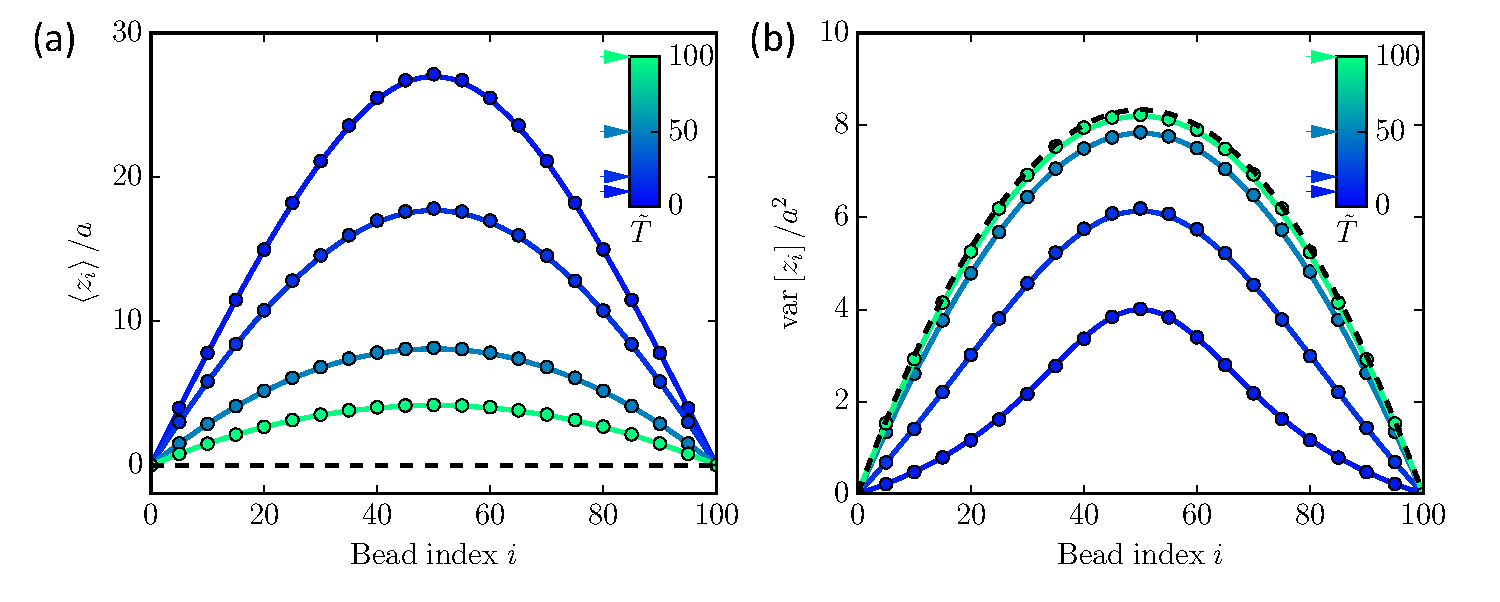
\includegraphics[width=1.0\linewidth]{meanVarZ3D}
    \caption{Mean and variance of the bead position in the direction along the force field. Solid lines are theory and dots are Monte-Carlo simulation results. The black dash line indicates the case $\tilde{T}\rightarrow\infty$, i.e. no external force field.}
    \label{fig:meanVarZ3D}
\end{figure}

Now let us discuss the directions perpendicular to the force direction. By symmetric reasons, we can immediately conclude that the statistics in $x$ and $y$ directions are identical. In addition, the mean position in both direction should be vanished because there is no bias. We can write as
\begin{equation}
    \label{eq:xyMean}
    \left<x_k\right> = \left<y_k\right> = 0.
\end{equation}

On the other hand, using Eq. \eqref{eq:second_moment}, the variance of $x$ and $y$ components of the $j^{\rm{th}}$ rod orientation can be written as
\begin{equation}
    \label{eq:xyRodVar}
    \text{var}\left[u_{j,x}\right] = \text{var}\left[u_{j,y}\right] = \left<u_{j,x}^2\right> - \left<u_{j,x}\right>^2 = (1-\left<\cos^2\theta_j\right>)/2
\end{equation}
Again, impose the Brownian bridge condition similar to Eq. \eqref{eq:varBrownianBridge3D}, the variance of $x$ and $y$ components of the bead position can be obtained. Notice the variance in $x$ and $y$ directions are different from the variance in $z$ direction. This is shown in Fig \ref{fig:xyVar3D} together with the benchmark of our theory and the Monte-Carlo simulations.

\begin{figure}[htpb]
    \centering
    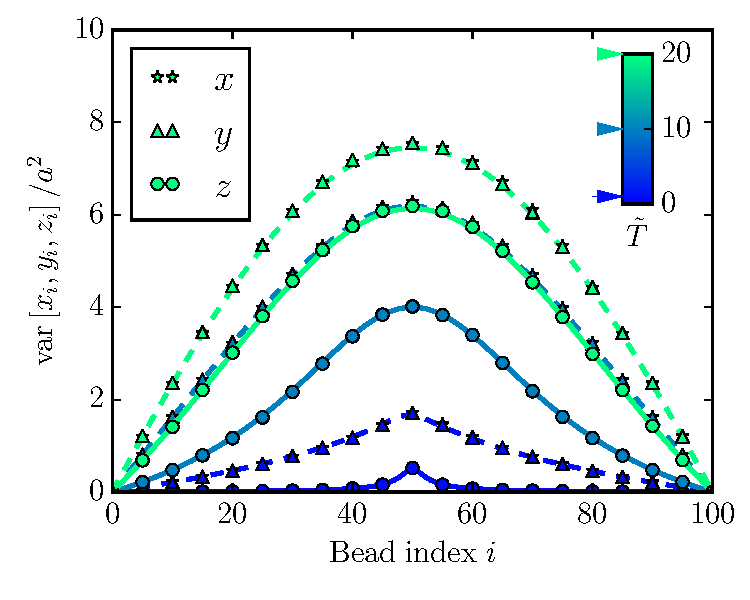
\includegraphics[width=0.6\linewidth]{xyVar3D}
    \caption{Comparison of fluctuations in $x$, $y$ and $z$ directions. Symbols denote the Monte-Carlo simulations. Circles show the fluctuations along the $z$ axis, whereas stars and triangles along $x$ and $y$ axis respectively. Colors correspond to different dimensionless temperatures. Solid and dashed lines are theoretical predictions for fluctuations along and orthogonal to the force field, respectively.}
    \label{fig:xyVar3D}
\end{figure}


\subsection{The pairing of loops and intersecting loops}
\label{sub:the_pairing_of_loops_and_intersecting_loops}

In fission yeast, the chromosomes are appearing in pairs during nuclear oscillation, which means there are two mechanically identical chromosomes. And there are three chromosome pairs in fission yeast in total. The biological facts motivate us to consider a pair of polymer loops pinned at the same point. 
Biologically, recombination happens during nuclear oscillation. It is essential for homologous to come close spatially in order to recombine, which is done by a paring process. Thus it is meaningful to study to statistical distance between two corresponding loci along the polymer loops.
Physically, the pairing process of homologous is often said to be analogy to the zipping process of a zipper~\cite{Tsai2011}. Namely, segments near to the SPB are paired in prior. However, biologists suspect some additional connections between homologous could have been formed before the paring. And one of the hypothesises is that the centromeres of homologous are still bond together during nuclear oscillation. So these facts motivate us to consider the intersecting polymer loops with the same pinned point. In this subsection, we will calculate these cases in the 3D settings.

Firstly, let us discuss the paring of two identical polymer loops pinned at the same point. Fig. \ref{fig:pair} is the schematic of this case.
\begin{figure}[htpb]
    \centering
    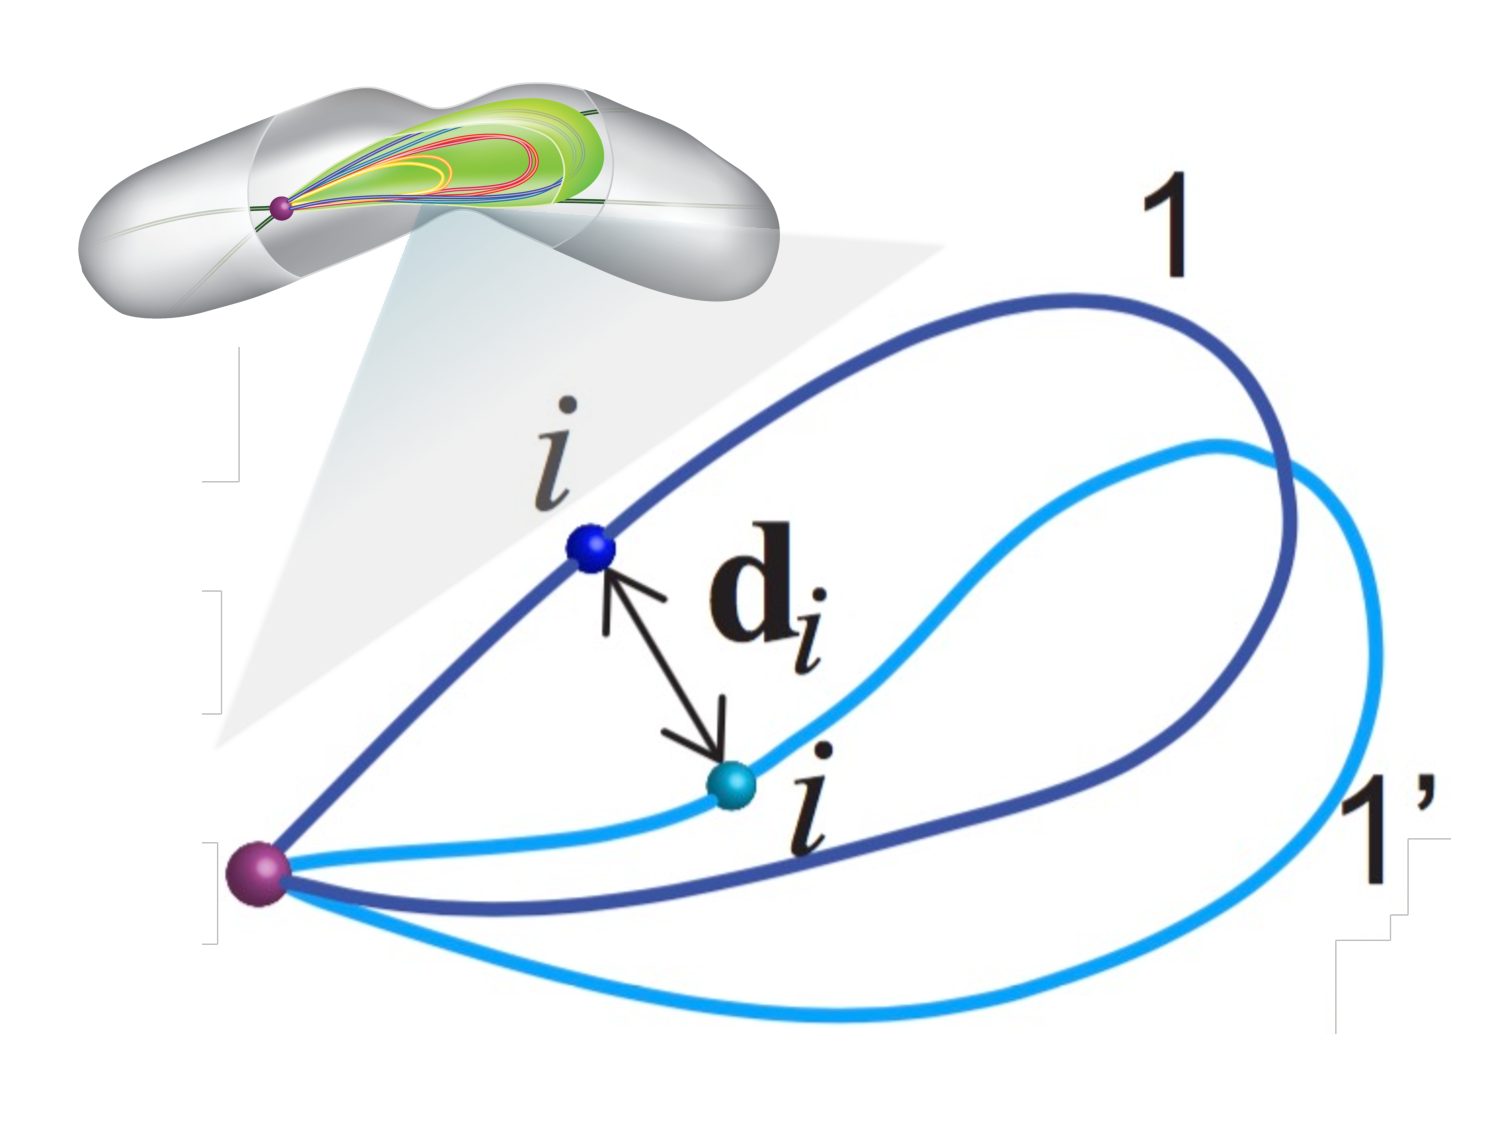
\includegraphics[width=0.6\linewidth]{pairLoops}
    \caption{A Pair of polymer loops pinned at the same point representing the homologous. The distance of a pair of loci is illustrated as $\mathbf{d}_i$. }
    \label{fig:pairLoops}
\end{figure}

Given that the excluded volume effect is ignored, the three dimensional mean distance between two corresponding beads is zero. The statistical distance is defined as the square root of its variance and the variance is calculated as:
\begin{equation}
    \label{eq:statisticalDistance}
    \text{var}\left[\mathbf{d}_i\right] = 
    \text{var}\left[\mathbf{r}_i - \mathbf{r}_i^\prime\right] = 2 \text{var}\left[\mathbf{r}_i\right]
    = 2\left( \text{var}\left[x\right] + \text{var}\left[y\right] + \text{var}\left[z\right]\right).
\end{equation}
In Fig.~\ref{fig:pairing} we show the statistical distance varies with the dimensionless temperature, which is the inverse measure of the external force field strength.
We can see from the figure that strong force field reduces the statistical distance thus facilitates pairing. BD simulations are performed and results are found match to our theory. 
\begin{figure}[htpb]
    \centering
    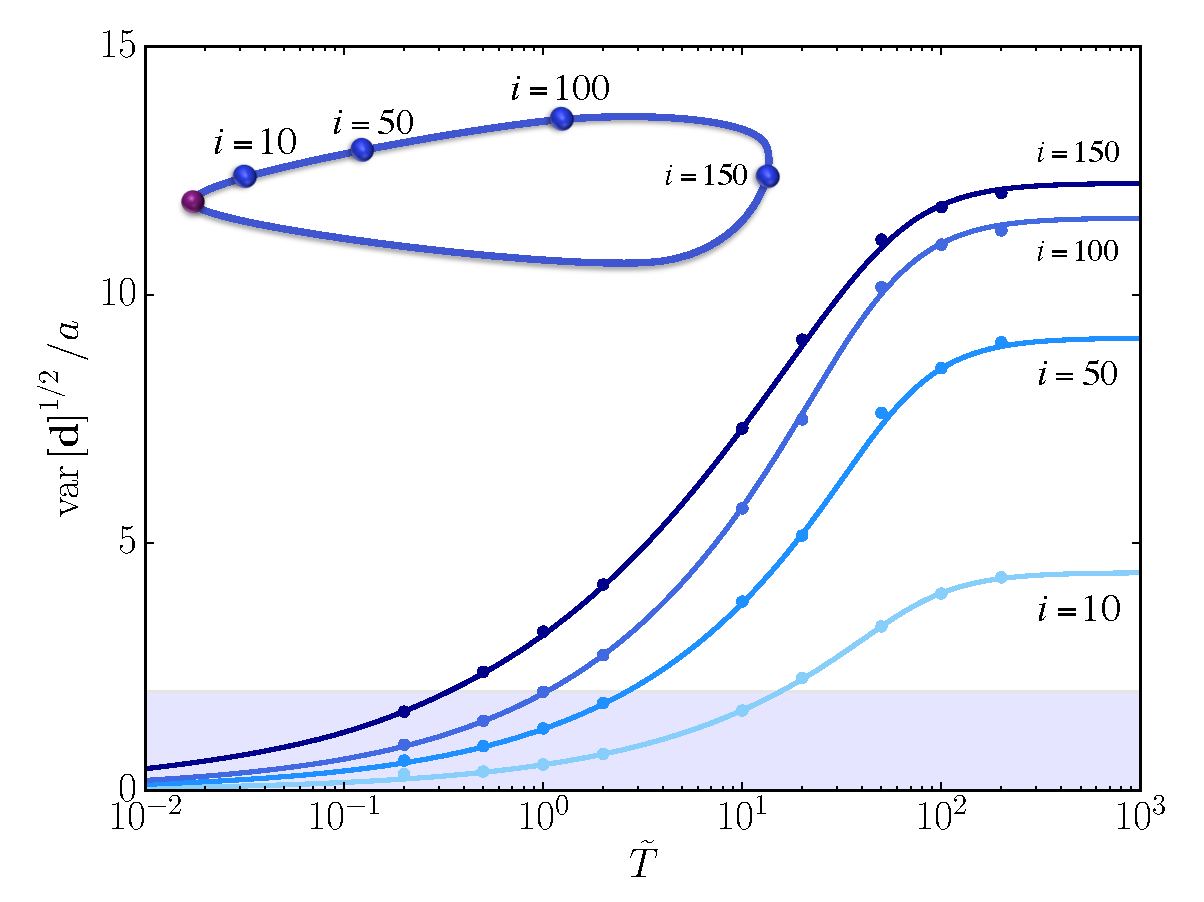
\includegraphics[width=0.7\linewidth]{pairing}
    \caption{The distance between corresponding loci of polymer pair loops varies withe the dimensionless temperature. Different curve indicates different location along loop. The shaded region the paired distance. Dots are BD simulation data and solid lines are results from our theory. Inset is an sketch of the observing loci along the chromosome. $L=300,~k_BT=1$ are set.}
    \label{fig:pairing}
\end{figure}

Now let us discuss the case of pairing with an additional intersecting in the middle of polymer loops. The schematic of this case is shown in Fig.~\ref{fig:centromere}.
\begin{figure}[htpb]
    \centering
    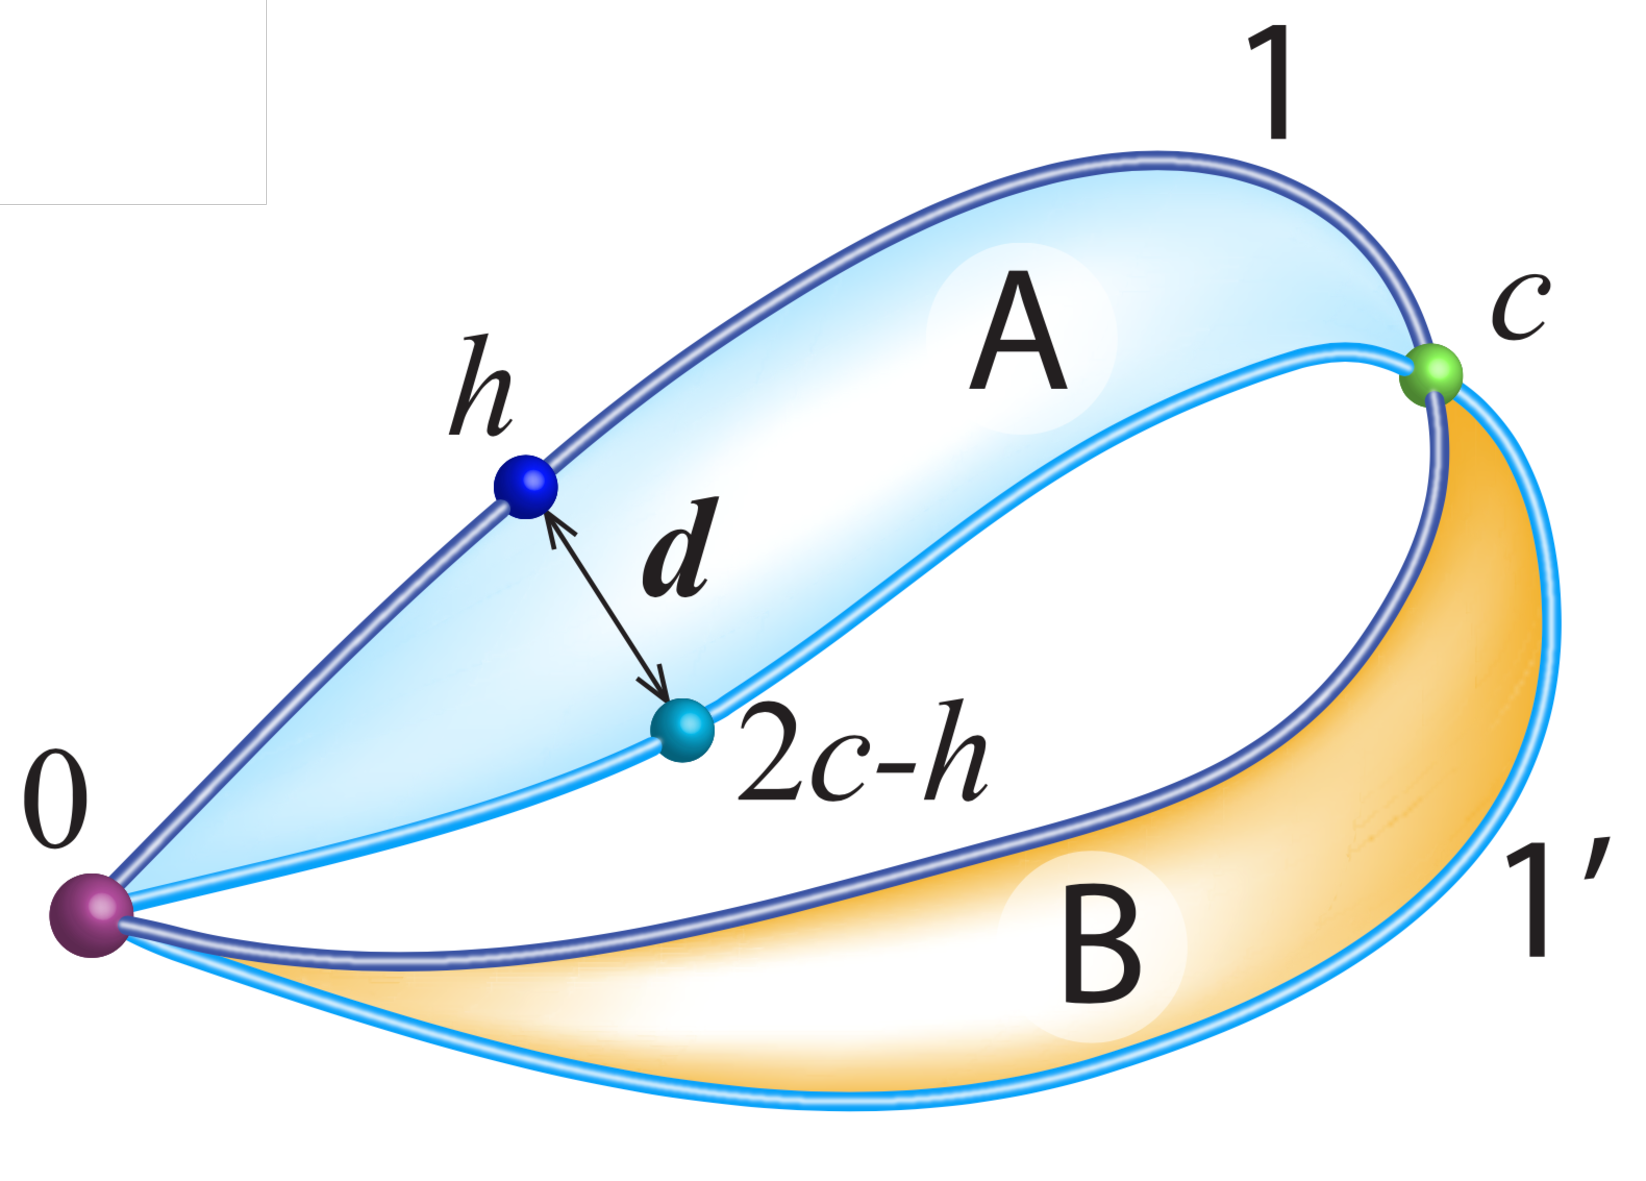
\includegraphics[width=0.6\linewidth]{centromere}
    \caption{The sketch of two intersecting loops $1$ and $1^\prime$ which are connected at one additional bead with index $c$. Shaded regions indicate the redefined loops A and B. The distance $\mathbf{d}$ between two homologous beads $h$ and $2c-h$ is illustrated. }
    \label{fig:centromere}
\end{figure}
The pair of polymer loops (denoted by $1$ and $1^\prime$) pinned at the same point $0$ with an additional constraint at some intermediate bead position (indexed by $c$, where $0<c<L$). However, bead $c$ is not pinned so that it can still move around. 

In order to solve this problem, we redefine the loops as shown in Fig.~\ref{fig:centromere}. The loop A starts at the pinned point, continues along the loop $1$, to the constraint point $c$ and then returns to the origin along the loop $1^\prime$ by the path of the same length. It is shown in Fig.~\ref{fig:centromere} shaded with cyan color in between. The loop B is shown in Fig.~\ref{fig:centromere} shaded with orange color in between. We are interested in the distance $\mathbf{d}$ between two homologous beads as shown in the figure. Denote the first bead position with index $h$, then the other one can be denoted by $2c-h$ considering the loop A. 
\begin{figure}[htpb]
    \centering
    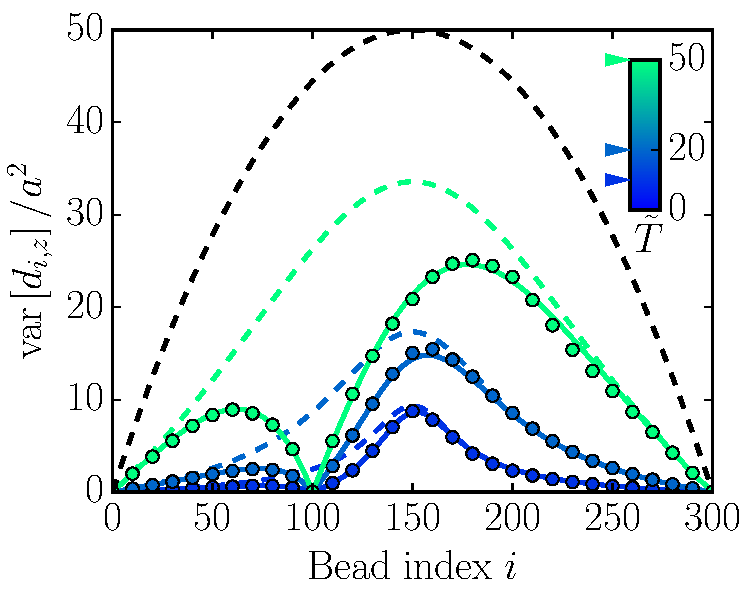
\includegraphics[width=0.6\linewidth]{varCentromere}
    \caption{Variance of the distance between pinned polymer loops with additional constraint. The constraint is located at the bead with index $c=100$. Circles denote the simulation results while the solid lines represent the theory. The dashed lines show the variance of the unconstrained case with different color indicates different dimensionless temperature. The black dashed line shows the limit of unconstrained force-free Brownian bridge.}
    \label{fig:varCentromere}
\end{figure}

To calculate the PDF of $\mathbf{d} := \mathbf{r}_h - \mathbf{r}_{2c-h}$, which denote as $\rho(\mathbf{d})$, let us first calculate the joint positional PDF $\rho_{h, 2c-h}(\mathbf{r}_1, \mathbf{r}_2)$. Denote the propagator as $\rho_{k\rightarrow j}(\mathbf{r}_1 | \mathbf{r}_2) = \rho(\mathbf{r}_k = \mathbf{r}_1 | \mathbf{r}_j = \mathbf{r}_2)$. Notice that the propagator is a (multi-variate) Gaussian function with a mean and variance summing up by path steps. Then we can apply the similar Brownian bridge condition, obtaining
\begin{equation}
    \label{eq:jointPdfDistance}
    \rho_{h,2c-h}(\mathbf{r}_1, \mathbf{r}_2) = \frac{\rho_{0\rightarrow h}(\mathbf{r}_1|0)\rho_{h\rightarrow 2c-h}(\mathbf{r}_1|\mathbf{r}_2)\rho_{0\rightarrow 2c-h}(\mathbf{r}_2|0)}{\rho_{0\rightarrow 2c}(0|0)}.
\end{equation}
And then the PDF $\rho(\mathbf{d})$ can be calculated as 
\begin{equation}
    \label{eq:pdfDistance}
    \rho(\mathbf{d}) = \int\int d\mathbf{r}_1 d\mathbf{r}_2 \delta(\mathbf{d} - (\mathbf{r}_1 - \mathbf{r}_2))\rho_{h, 2c-h}(\mathbf{r}_1, \mathbf{r}_2),
\end{equation}
Without evaluate the integrals in Eq. \eqref{eq:pdfDistance}, one can conclude $\rho(\mathbf{d})$ is Gaussian because $\rho_{h,2c-h}(\mathbf{r}_1, \mathbf{r}_2)$ is Gaussian. It is not difficult to obtain the mean distance is $\left<\mathbf{d}\right>=\mathbf{0}$ because of no excluded volume effect. And the variance can calculate the same way as our previous procedure. For example, the $z$-component variance is
\begin{equation}
    \label{eq:zvarDistance}
    \text{var}\left[ d_z \right] = 2 \frac{\sigma_{0\rightarrow h,z}^2\sigma_{h\rightarrow c,z}^2}{\sigma_{0\rightarrow c,z}^2}, 
\end{equation}
where each variance is calculated according to Eq. \eqref{eq:meanVarRod}. The result compare with simulations is shown in Fig. \ref{fig:varCentromere}. We see that fluctuations of the distance is reduced with the additional constraint point compared with the unconstrained case. 

In this section, we discussed the three dimensional pinned polymer loop model and its equilibrium statistics. The mean and variance of each bead position are calculated using the grand canonical ensemble combined with Brownian bridge technique. 
Fluctuations of distance between corresponding beads of pinned polymer pair loops are calculated analytically to quantify the paring process. The theoretical results are all verified by simulations. In addition, by discussing the case of two intersecting polymer loops, we find the additional constraint helps to reduce the fluctuations, thus facilitate the pairing process. 
In next section, we will use the theory of equilibrium statistics to quantify the shape of polymer loops in an external force field.


%********************************** % Fourth Section  *************************************
\section{Characterizing the shape of pinned polymer loops}
\label{sec:characterizing_the_shape_of_pinned_polymer_loops}

We have shown the in Fig. \ref{fig:oscillation} the stained chromosomes during nuclear oscillation. Experimentally, it is relatively easier to measure the shape of the chromosomes. 
On the other hand, the shape of the chromosomes is believed to be important for the paring process of homologous. For example, it is reported in \cite{Chacon2016} that the expression of the LinE protein Rec25 is promoted in elongated nucleus than the round shaped nucleus. So it is meaningful to characterize the shape of the chromosomes quantitatively. 

In this section, we will introduce several indicators used to quantify the shape of steady state chromosomes, which is modeled by the pinned polymer loops. We will introduce the three dimensional gyration tensor, asphericity and the nature of asphericity. The simulation results are compared with the theory from preceded sections. We will also try to compare our theory to the blob theory, which is known as the ``stem-flower'' shape of pinned polymer chain. 


\subsection{The gyration tensor}
\label{sub:the_gyration_tensor}
Before the study of the pinned polymer shape, let first have a look of the simulation results for the polymer shape in several typical cases. 

\begin{figure}[htpb]
    \centering
    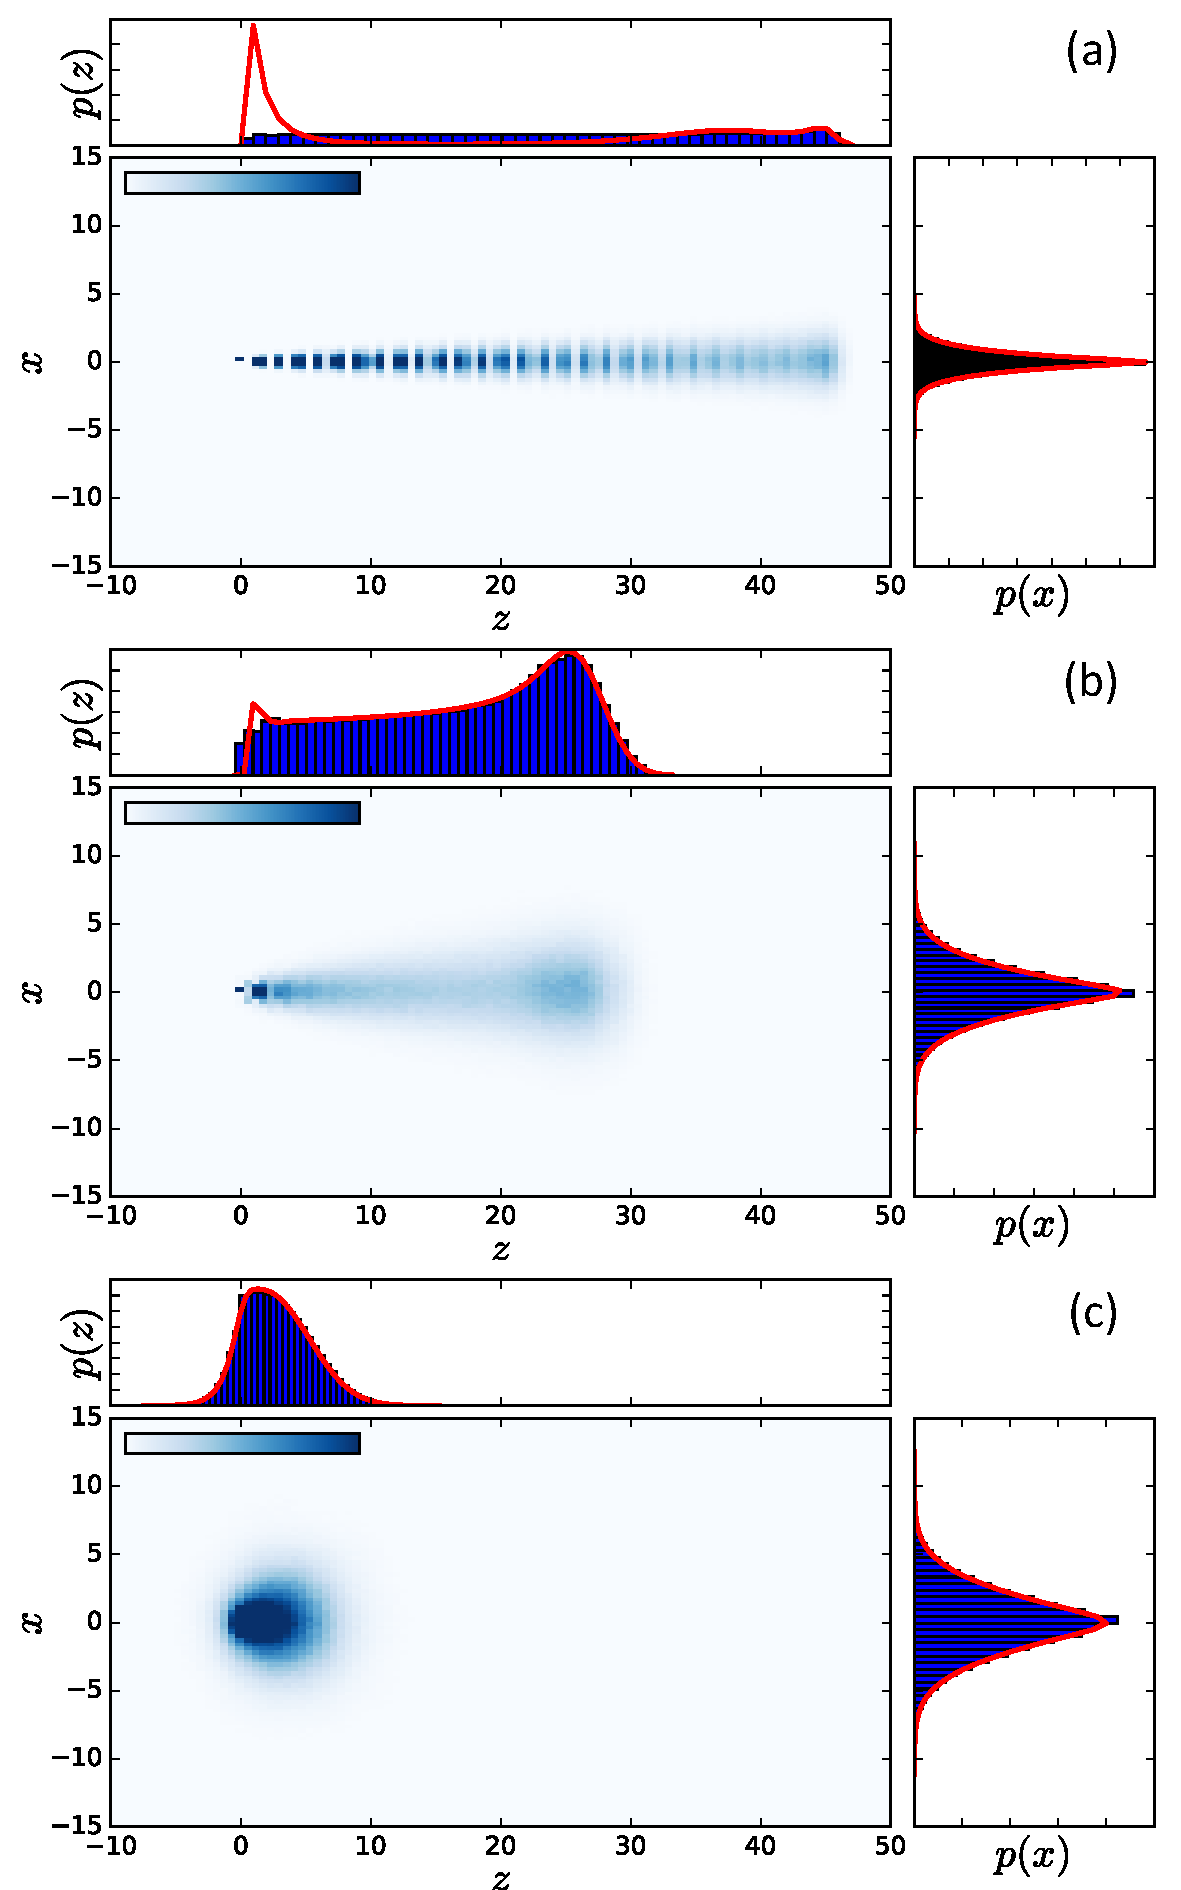
\includegraphics[width=0.9\linewidth]{shapeCases}
    \caption{The density distribution of pinned polymer shape for (a) strong external force field with $F=1$, (b) moderate external force field with $F=0.1$, (c) weak external force field with $F=0.01$. Other parameters are set as following $a=1,~k_B T = 1,~L=100$. See more explanations in the main text.}
    \label{fig:shapeCases}
\end{figure}

We show in Fig. \ref{fig:shapeCases} the monomer density distribution of a 3D pinned polymer loop projected in the 2D $x-z$ plane. 
The upper panel shows the marginal distribution of density along the force direction $z$ axis, while the right panel shows the marginal distribution of density perpendicular to the force direction along $x$ axis. The red lines represent the theoretical results which we will discuss next.

In section \ref{sec:equilibrium_statistics_in_3d}, we show the mean and variance of the bead position in 3D. When the dimensionless temperature is not too small ($\tilde{T}\gg 1$), the distribution of of the bead position can be considered as Gaussian. So we have
\begin{subequations}
    \label{eq:posDistribution}
    \begin{align}
    p(z_i) & = \frac{1}{\sqrt{2\pi \text{var}\left[z\right]_i}} \exp\left(-\frac{(z_i - \left<z_i\right>)^2}{2\text{var}\left[z_i\right]}\right), \\
    p(x_i) & = \frac{1}{\sqrt{2\pi \text{var}\left[x\right]_i}} \exp\left(-\frac{(x_i - \left<x_i\right>)^2}{2\text{var}\left[x_i\right]}\right).
    \end{align}
\end{subequations}
And then the marginal particle density can be calculated as
\begin{subequations}
    \label{eq:particleDensity}
    \begin{align}
        P(z) & = \frac{1}{L} \sum_{i=1}^L p(z_i), \\
        P(x) & = \frac{1}{L} \sum_{i=1}^L p(x_i).
    \end{align}
\end{subequations}
Substitute the mean and variance we obtained in section \ref{sec:equilibrium_statistics_in_3d}, the theoretical results of red lines in Fig. \ref{fig:shapeCases} can be obtained. Notice that the theory of $p(z)$ fits not so good with the simulation results in Fig. \ref{fig:shapeCases} (a), and it is because the Gaussian assumption is not valid in the strong force regime along the force direction. 

Although the density profile of monomers can be calculated as above, the intuition of the polymer shape is still unclear. In order to quantify the shape and get an intuition, we calculate the 3D gyration tensor of the polymer, which is defined as following:
\begin{equation}
    \label{eq:gyrationTensor}
    Q = \begin{bmatrix}
    Q_{xx} & Q_{xy} & Q_{xz} \\
    Q_{yx} & Q_{yy} & Q_{yz} \\
    Q_{zx} & Q_{zy} & Q_{zz} 
    \end{bmatrix}
    \rightarrow \begin{bmatrix}
    \lambda_{x}^2 & 0 & 0 \\
    0 & \lambda_{y}^2 & 0 \\
    0 & 0 & \lambda_{z}^2 
\end{bmatrix}
\end{equation}
where the elements $Q_{xy}$ can be written as 
\begin{equation}
    \label{eq:gyrationTensorElement}
    Q_{xy} = \frac{1}{L}\sum_{i=1}^L{(x_i-x_{CM})(y_i-y_{CM})},
\end{equation}
and $x_{CM}$ is the $x$ component of the center of mass vector. The right arrow in Eq.~\eqref{eq:gyrationTensor} means the diagonalization, and $\lambda_x^2, ~\lambda_y^2, ~\lambda_z^2$ represent the three non-negative eigenvalues of the gyration tensor. Physically, the intuition of the three eigenvalues can be interpreted as the magnitude of three orthogonal axes of the fitted ellipsoid enclosing the polymer loops. For convenience, we order them by $\lambda_x^2\leq\lambda_y^2\leq\lambda_z^2$.

Based on the gyration tensor, the first shape indicator we want to discuss is the gyration radius of the polymer, which is defined and can be calculated as following:
\begin{equation}
    \label{eq:gyrationRadius}
    R_g^2 :=  \frac{1}{L} \sum_{i=1}^L \left(\mathbf{r}_i - \mathbf{r}_{CM}\right)^2 = \lambda_x^2 + \lambda_y^2 + \lambda_z^2
\end{equation}

\begin{figure}[htpb]
    \centering
    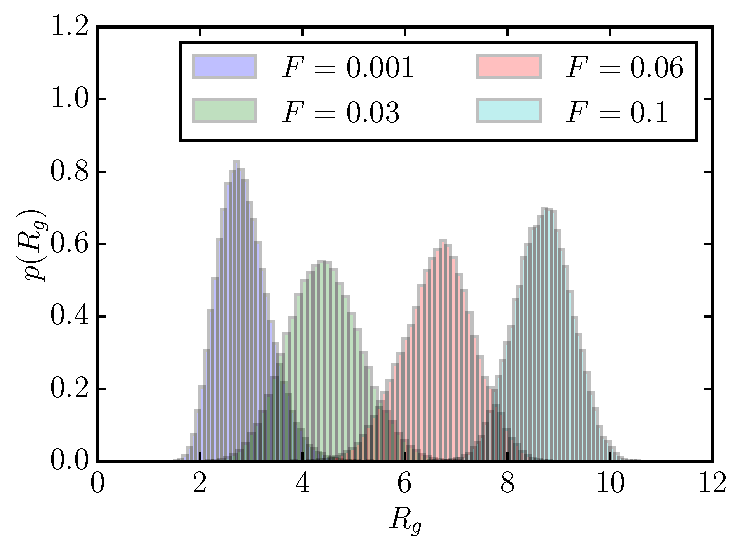
\includegraphics[width=0.8\linewidth]{rgpdf}
    \caption{The distribution of gyration radius of pinned polymer loop under different strength of external force field. $L=100, ~k_BT=1$. }
    \label{fig:rgpdf}
\end{figure}
In Fig. \ref{fig:rgpdf}, we show the distribution of gyration radius under several force field. Interestingly, we can see that the width of the distribution varies non-monotonically with the strength of external force. In other words, the gyration radius is more fluctuating under a moderate force field. 
The explanation for the unexpected non-monotonic behavior is the symmetry break because of the pinned effect. We can see in Fig. \ref{fig:shapeCases} (b) that the free end of the polymer is more fluctuating while the pinned end is fixed. This leads to a trumpet-like shape of the polymer. So we have the with of the distribution varies non-monotonically with the external fore field.

In next subsection, we will introduce two more descriptors of the polymer shape, which is the asphericity and the nature of asphericity.

\subsection{Asphericity and the nature of asphericity}
\label{sub:asphericity_and_the_nature_of_asphericity}

The asphericity and the nature of asphericity are two descriptors that commonly used to quantify the shape of the polymer. The definition of them are based on the gyration tensor \cite{Alim2007}. More specifically, the asphericity is defined by
\begin{equation}
    \label{eq:asphericity}
    \Delta = \frac{3}{2} \frac{\text{Tr}\hat{Q}^2}{(\text{Tr}Q)^2},
\end{equation}
where $\hat{Q}_{ij} = Q_{ij} - \delta_{ij}\text{Tr}Q/3$. The nature of asphericity is given by
\begin{equation}
    \label{eq:natureAsphericity}
    \Sigma = \frac{4\det\hat{Q}}{\left(\frac{2}{3}\text{Tr}\hat{Q}^2\right)^{3/2}}.
\end{equation}
However, in order to compare the shape of the pinned model with the researches in the literature \cite{Alim2007,Blavatska2010a}, we adopt the parameter $\rho = 2\sqrt{\Delta} \in [0,2]$ and $\theta = \arccos\Sigma/3\in[0,\pi/3]$. The physical interpretation of these parameters are illustrated in Fig. \ref{fig:shapeDistr} (a). Basically, $\rho=0$ corresponds to a fully spherical object while $\rho=2$ means the shape of the object is rod-like. And $\theta$ measures whether the object is prolate or oblate. 

\begin{figure}[htpb]
    \centering
    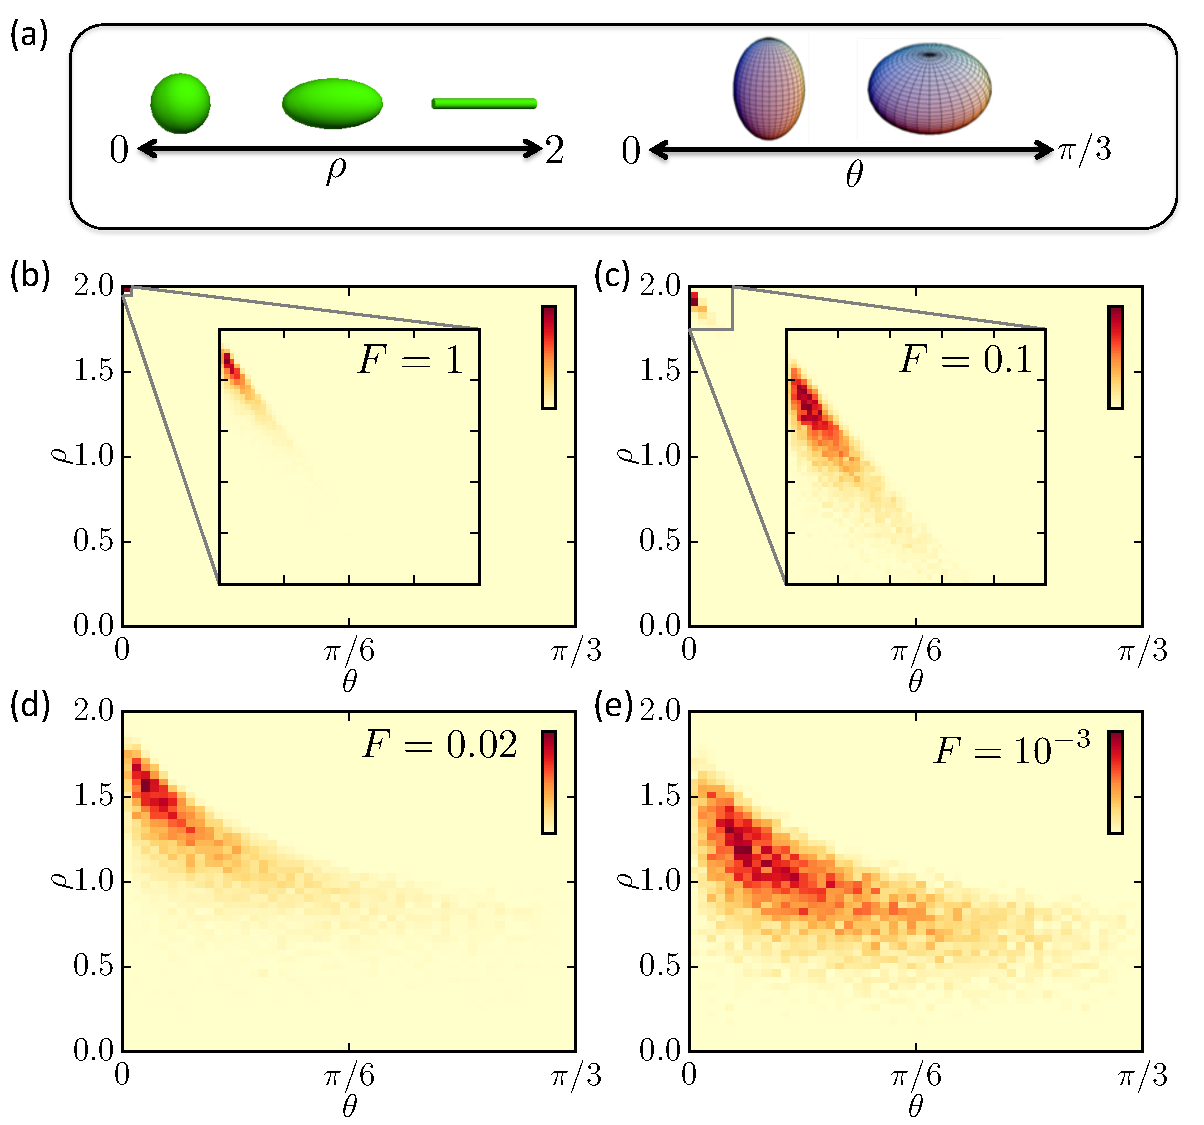
\includegraphics[width=1.0\linewidth]{shapeDistr}
    \caption{The shape of pinned polymer loop distributed over the phase diagram of asphericity and the nature of asphericity. (a) The intuition of asphericity and the nature of asphericity are illustrated. (b) The $\rho-\theta$ phase diagram for $F=1$. (c) The $\rho-\theta$ phase diagram for $F=0.1$. (d) The $\rho-\theta$ phase diagram for $F=0.02$. (e) The $\rho-\theta$ phase diagram for $F=0.001$. Other parameters such as $k_B T =1,~L=1,~a=1$.}
    \label{fig:shapeDistr}
\end{figure}

As we can see from Fig. \ref{fig:shapeDistr}, the shape of the pinned polymer loop is spread over a sickle-shaped area. In addition, the prolate and elongated shape is preferred no matter the external force is strong or not. The phase diagrams we found here are similar to those of semi-flexible unpinned polymer loops in \cite{Alim2007}.

In this section, we introduce several shape descriptors of pinned polymer loop based on the 3D gyration tensor. The theory monomer density distribution is also shown and compared to the Monte-Carlo simulation data and a good consistency is obtained. 



%********************************** % Sixth Section  *************************************
\section{Summary}
\label{sec:summary_chp3}

In this chapter, we discuss the equilibrium statistics of pined polymer loops in an external force field, which is our model for chromosomes in meiotic fission yeast. 

We first solve the statistics in a idealized 1D model. We introduce a technique which combines the \emph{Fermi-Dirac} statistics and Brownian Bridge condition to solve the problem in \emph{grand} canonical ensemble. The solution found is compared to the exact solution, which can be obtain after utilize the analogy to a number partition problem. However, we found that the results from our technique are quite accurate and the exact solution is quite cumbersome for later calculations. Thus the first approach is preferred. Using the result, we are able to calculate the mean and variance of bead position.  

And then we extend our theory to the three dimensional system. The same method of Brownian Bridge is used to solve the statistics. Also the three dimensional mean and variance of bead position is calculated. Moreover, the paring of polymer loops pinned at the same point is discussed. We calculate the statistical distance of the corresponding loci along the polymer loops. We found that the distance is reduced efficiently by the external force field. Thus the mechanism of facilitating pairing by pulling is illustrated. In addition, we also calculate the intersecting polymer loops in order to study the role of more constraints in the paring process. And the conclusion is additional constraints further reduce the fluctuation and facilitate the pairing. 

In the last section, we use our theoretical results to discuss the shape of pinned polymer loops in an external force field. The approximation for marginal distribution of monomer density is calculated in both parallel and transverse directions. And we quantify the shape based one the three dimensional gyration radius. Interestingly, we found the width of gyration radius distribution varies non-monotonic with the strength of the external force field. The phase diagram of asphericity and the nature of asphericity were shown which implies a rod-like and prolate shape of the pinned polymer loops in both weak and strong force field.

In next chapter, we will delve deeper to study the non-equilibrium properties of the pinned polymer loop polymer in an external force field. 

\chapter{Dynamical Properties of Pulled Polymer Loops}
\graphicspath{{Chapter4/Figs/}}

In previous chapter, the equilibrium statistics of pinned polymer loops in an external force field are discussed in details. However, we known that the nuclear oscillation in fission yeast is of course a non-equilibrium process. So we have to assume the relaxation time of the system is much smaller than the oscillation period to make our discussion reasonable. The assumption need to be justified. On the other hand, it is interesting to know the dynamical properties of pinned polymers in an external field from theoretical point of view. To the best of our knowledge, the way to calculate the relaxation time of a pinned bead-rod model is still missing. 

In this chapter, we will study the dynamical properties of pinned polymer loop model representing the chromosomes in fission yeast. We will verify our assumption of short relaxation time used in previous chapter. Using the Rouse theory, we first study the pinned bead-spring polymer loop in an external force field. Then using the mapping from bead-rod polymer to the particle-lattice picture, we calculate the full dynamics of the 1D system. The Bethe-ansatz method is utilized to solve the dynamics. Excellent results is obtained and compared to the projection of 3D polymer results from BD simulations. 

In the first section, we illustrate how to apply the Rouse theory on our pinned polymer loop model in an external filed. In the second section, we introduce the mapping from 1D polymer dynamics to the ASEP (Asymmetric Simple Exclusion Process). An brief background knowledge of ASEP is introduced. In the third section, we use the Bethe-ansatz method to solve the ASEP problem exactly and calculate the relaxation time analytically. In the force section, we try to apply our calculation to the 3D bead-rod model. Finally, a summary is given in the last section. 



%********************************** %First Section  **************************************
\section{Rouse theory of the pinned bead-spring loop}
\label{sec:rouse_theory_of_the_pinned_bead_spring_loop}
Rouse theory is a theoretical framework to calculate the dynamics of a polymer. Comparing to other theory like the Zimm theory, it is simple and gives the full information of dynamics. In most cases, Rouse theory can apply only to the bead-spring model. This is one of the reason that the bead-spring model is more popular than the bead-rod model. 

In the case of modeling chromosomes in fission yeast, we intend to use the bead-rod model instead of the bead-spring. This is mainly because the finite extensibility, which is important for condensed meiotic chromosomes, can be described easily by the bead-rod model. However, the study of Rouse theory is still useful because of several reasons. On one hand, we will see later that Rouse theory can correctly represent the zero external force limit of the bead-rod model. On the other hand, in realistic simulation that take into account many complex factors, it is not so important whether the bead-rod or bead-spring model is utilized. In this case, the simple rouse theory offers an theoretical calibration line for us to analyze the polymer system.

Despite the simplicity of the Rouse theory, we have not seen a calculation of the Rouse theory on the pinned polymer loop model. So what we present here is new. Let us start by writing down the dynamical equations of the model.  

\subsection{Dynamical equations}
\label{sub:dynamical_equations}
\begin{figure}[htpb]
    \centering
    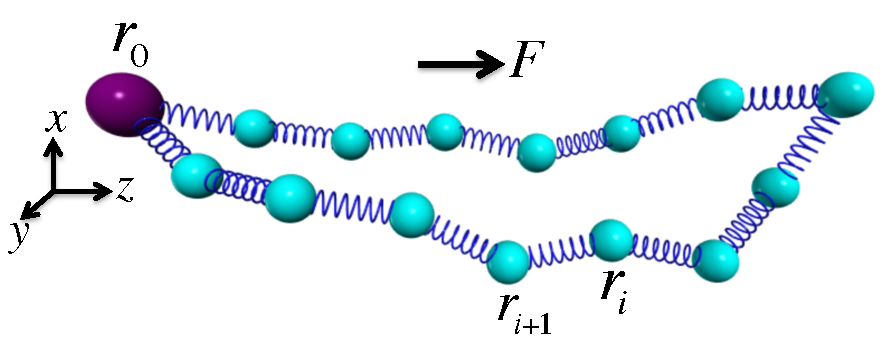
\includegraphics[width=0.8\linewidth]{beadspring}
    \caption{The sketch of pinned bead-spring loop with notations. }
    \label{fig:beadspringNotation}
\end{figure}

Consider a pinned polymer loop modeled by beads and connecting springs, see in the sketch Fig. \ref{fig:beadspringNotation}. As in our previous discussion of the bead-rod model, the bead labeled by $0$ is assumed be pinned at the origin and there are $L$ beads in total in the loop. Again the periodic indexing is used. We can write the pinned condition as $\mathbf{r}_0 = \mathbf{r}_L = \mathbf{0}$.

The dynamical equation for a single bead in the loop is Eq. \eqref{eq:beadspringEq}. However, we rewrite it as following after considering the connecting structure:  
\begin{equation}
    \label{eq:beadspringConnect}
    \xi \frac{d \mathbf{r}_i}{dt} = - k_H \sum_{k} A_{ik} \mathbf{r}_k + \mathbf{f}_i^e + \mathbf{f}_i^b,
\end{equation}
where $\xi$ is the friction coefficient of bead in solution, $\mathbf{r}_i$ is the bead position of the $i$th bead, $k_H$ is the spring constant with a linear Hookean spring assumed. $\mathbf{f}_i^e$ is the external force exerted on beads, $\mathbf{f}_i^b$ is typical Brownian force satisfying Eq. \eqref{eq:brownianforce}.
$\mathbf A$ is the connecting matrix. It is not difficult to find that in the case of the setting above, i.e. pinned loop, $\mathbf{A}$ is a $(L-1)\times (L-1)$ matrix and has the following form
\begin{equation}
    \label{eq:connectMatrix}
    \mathbf{A} = \begin{bmatrix}
        2 & -1 & 0   & \cdots   \\
        -1 & 2 & -1  &  \cdots  \\
        \vdots & \ddots &\ddots&\vdots\\
        \cdots & -1 &2 & -1 \\
        \cdots & 0 &-1 &2
    \end{bmatrix}.
\end{equation}

Notice that we do not take into account any complex terms of interaction such as bending stiffness and exclusive effect in this simple model. This is because analytical results are tractable in such a simple Rouse setting. The impact of these complex interaction terms will be studied numerically by BD simulation in next chapter. 

\subsection{The normal modes}
\label{sub:the_normal_modes}
For convenience, we use the vector notation and rewrite Eq. \eqref{eq:beadspringConnect} as:
\begin{equation}
    \label{eq:beadspringVector}
    \xi \frac{d }{dt} \mathbf{R} = - k_H \mathbf{A} \mathbf{R} + \mathbf{F}^e + \mathbf{F}^b,
\end{equation}
where $\mathbf{R} = \left[\mathbf r_1, \mathbf r_2, \cdots, \mathbf r_{L-1}\right]^T$, and similar vector notation is also applied for $\mathbf{F}^e$, $\mathbf{F}^b$. In order to solve this set of dynamical equations, we first notice that the connecting matrix $\mathbf{A}$ is a very special type of matrix called tridiagonal Toeplitz matrix \cite{meyer2000}. Fortunately, it can be diagonalized exactly. To do this, let us introduce a similarity transfer that
\begin{equation}
    \label{eq:similarityTransfer}
    \left[\Omega^{-1} \mathbf{A} \Omega\right]_{jk} = \mathbf{D}_{jk} = \lambda_k\delta_{jk},
\end{equation}
here $\Omega$ is normalized to be a unitary matrix, and $\lambda_k$ is the eigenvalue of matrix $\mathbf A$. We skip the calculation details here and just give out the results as following
\begin{subequations}
    \begin{align}
    \lambda_k  & =  4\sin^2\left(\frac{k\pi}{2 L}\right), k = 1, 2, \cdots, L-1; \\
    \Omega_{jk} & =  \Omega_{kj} = [\Omega^{-1}]_{jk} = [\Omega^{-1}]_{kj} = \sqrt{\frac{2}{L}}\sin\left(\frac{jk\pi}{L}\right).
    \end{align}
\end{subequations}
Then we can multiply both sides of Eq. \eqref{eq:beadspringVector} by $\Omega^{-1}$ arrive at
\begin{equation}
    \label{eq:beadVectorTransfer}
    \xi\frac{d(\Omega^{-1}\mathbf{R})}{dt} = 
    -k_{H}\Omega^{-1} \mathbf{A}\Omega\Omega^{-1} \mathbf{R} + \Omega^{-1}\mathbf{F}^e + \Omega^{-1}\mathbf{F}^b.
\end{equation}
Notice that $\Omega^{-1}\mathbf{A}\Omega = \mathbf{D}$ and use the notation such that $\tilde{\mathbf{R}} = \Omega^{-1} \mathbf{R}$, we get the set of decoupled dynamical equations
\begin{equation}
    \label{eq:decoupledBead}
    \xi\frac{d\tilde{\mathbf{r}}_j}{dt} = -k_{H} \lambda_j \tilde{\mathbf{r}}_j + \tilde{\mathbf{f}}^e_j + \tilde{\mathbf{f}}^b_j.
\end{equation}
Eq. \eqref{eq:decoupledBead} can be solved easily by standard methods. The general solution can be written as following
\begin{equation}
    \label{eq:solutionTransformed}
    \tilde{\mathbf{r}}_j(t) = \tilde{\mathbf{r}}_j(0) e^{-\frac{k_H \lambda_j}{\xi} t} + \frac{1}{\xi}
    \left(\int^t_0{\tilde{\mathbf{f}}^e_j e^{-\frac{k_H \lambda_j}{\xi} (t -t^\prime)}} dt^{\prime} + \int^t_0{\tilde{\mathbf{f}}^b_j e^{-\frac{k_H \lambda_j}{\xi} (t -t^\prime)} }dt^{\prime} \right).
\end{equation}
Here the transformed Brownian force also fulfills 
\begin{subequations}
    \begin{align}
    \label{eq:brownianTransformed}
    \left<\tilde{\mathbf{f}}_j^b\right> & = \mathbf 0; \\
    \left<\tilde{f}_{i\alpha}^b(t)\tilde{f}_{j\beta}^b(t^\prime)\right> & = 2\xi k_B T \delta_{ij} \delta_{\alpha\beta}\delta(t-t^\prime).
    \end{align}
\end{subequations}
Given the solution of Eq. \eqref{eq:solutionTransformed}, the position of each bead can be obtain by the inverse transformation $\mathbf{R} = \Omega\tilde{\mathbf{R}}$. In the simple case of constant external force field, $\mathbf{f}_j^e = f^e \mathbf{e}_z$, Eq. \eqref{eq:solutionTransformed} can be rewritten as
\begin{equation}
    \label{eq:solutionTransformedConstant}
    \tilde{\mathbf{r}}_j(t) = \tilde{\mathbf{r}}_j(0) e^{-\frac{k_H \lambda_j}{\xi} t} + \frac{\tilde{f}^e\mathbf{e}_z}{k_H \lambda_j}\left(1-e^{-\frac{k_H \lambda_j}{\xi} t} \right) +\frac{1}{\xi} \int^t_0{\tilde{\mathbf{f}}^b_j e^{-\frac{k_H \lambda_j}{\xi} (t -t^\prime)} }dt^{\prime}
\end{equation}
Finally, the bead position can be obtained by the inverse transformation:
\begin{equation}
    \label{eq:beadPosRouse}
    \mathbf{r}_i (t) = \sum_j \Omega_{ij} \tilde{\mathbf{r}}_j(t)
\end{equation}

Now the equilibrium statistics of the polymer, such as the mean and variance of the each bead position can be calculated easily. Plug Eq.  \eqref{eq:solutionTransformedConstant} in Eq.  \eqref{eq:beadPosRouse} and let $t\rightarrow\infty$, we get 
\begin{equation}
    \label{eq:equilibriumBeadPosRaw}
    \left<\mathbf{r}_i^\infty\right> = \sum_j \Omega_{ij}
    \frac{\tilde{f}^e\mathbf{e}_z}{k_H \lambda_j} =
    \frac{f^e\mathbf{e}_z}{2 L k_H}\sum_{k,j}
    \frac{\sin\left(\frac{ij\pi}{L}\right)\sin\left(\frac{jk\pi}{L}\right)}
    {\sin^2\left(\frac{j\pi}{2L}\right)}.
\end{equation}
If $L\gg 1$, the summation of $j$ can be approximated by the integral so we get
\begin{equation}
    \label{eq:equilibriumBeadPos}
    \left<\mathbf{r}_i^\infty\right> = 
    \frac{f^e\mathbf{e}_z}{k_H} \sum_{k=1}^{\frac{L+1}{2}}\frac{\sin\left(\frac{i(2k-1)\pi}{L}\right)} {(2k-1)\pi\sin^2\left(\frac{(2k-1)\pi}{2L}\right)}.
\end{equation}
One can clearly see from Eq. \eqref{eq:equilibriumBeadPos} that $\left<\mathbf{r}_i\right> = \left<\mathbf{r}_{L-i}\right>$ as we expected. And the components of mean position perpendicular to the force field direction are vanished. 

In order to calculate the variance of bead position, it is nontrivial to firstly calculate the two time correlation of normal coordinate position, as following
\begin{equation}
    \begin{aligned}
    \label{eq:correlationTransformedPos}
    \left<\tilde{\mathbf{r}}_m(t)\tilde{\mathbf{r}}_n(t^{\prime})\right> = &
    \left<\tilde{\mathbf{r}}_m(0)\tilde{\mathbf{r}}_n(0)\right>
    e^{-\frac{k_h\lambda_m}{\xi}t-\frac{k_h\lambda_m}{\xi}t^{\prime}}  \\
    & + \frac{(\tilde{f}^e)^2}{k_H^2\lambda_m\lambda_n}
    \left(1 - e^{-\frac{k_H\lambda_m}{\xi} t} \right)
    \left(1 - e^{-\frac{k_H\lambda_n}{\xi} t^{\prime}} \right) \\
    & + \frac{3k_B T}{k_H\lambda_m}e^{-\frac{k_H\lambda_m}{\xi}t}\delta_{mn}.
    \end{aligned}
\end{equation}
Then the second moment of bead position can be calculated as:
\begin{equation}
    \label{eq:secondMoment}
    \left<\mathbf{r}_i^2(t)\right> = \sum_{m,n}\Omega_{im}\Omega_{in}
    \left<\tilde{\mathbf{r}}_m(t)\tilde{\mathbf{r}}_n(t)\right>.
\end{equation}
Finally, let $t\rightarrow\infty$, we get the equilibrium variance of bead position
\begin{equation}
    \label{eq:beadVariance}
    \text{var}\left[\mathbf{r}_i^{\infty}\right] =
    \left<(\mathbf{r}_i^{\infty})^2\right> - \left<(\mathbf{r}_i^{\infty})\right>^2 
    = \frac{3k_B T}{2 L k_H}\sum_{k=1}^{L-1}\left[ \frac{\sin\left(\frac{ik\pi}{L}\right)}
        {\sin\left(\frac{k\pi}{2L}\right)} \right]^2
    = \frac{3k_B T}{k_H L} i(L-i).
\end{equation}
Notice that we also have the symmetry that $\text{var}\left[\mathbf{r}_i^{\infty}\right] = \text{var}\left[\mathbf{r}_{L-i}^{\infty}\right]$. Moreover, it is important to point out the variance does not depend on the external force. So the statistical distance between two beads will not change no matter the external force filed is strong or weak. This is essentially because infinite extensible Hookean springs are employed in this simple model. 


\subsection{Relaxation time}
\label{sub:relaxation_time}
Besides the equilibrium statistics, dynamical properties are also tractable.  Our my interested quantity is the relaxation time of the pinned polymer. In order to do that, let us calculate the autocorrelation function of diameter vector, defined as $\mathbf{r}_d = \mathbf{r}_{\frac{L}{2}} - \mathbf{r}_0 = \mathbf{r}_{\frac{L}{2}}$. We can obtain 
\begin{equation}
    \label{eq:diameterVectorCorrelation}
    \left<\mathbf{r}_d(t)\mathbf{r}_d(0)\right> = 
    \sum_{m,n}\Omega_{\frac{L}{2}m}\Omega_{\frac{L}{2}}
    \left<\tilde{\mathbf{r}}_m(t)\tilde{\mathbf{r}}_n(0)\right>.
\end{equation}
From Eq. \eqref{eq:correlationTransformedPos} we can readily get the relaxation time 
\begin{equation}
    \label{eq:relaxationTimeRouse}
    \tau = \frac{\xi}{k_H\lambda_1} = \frac{\xi}{4k_H\sin(\pi/2L)},
\end{equation}
when $L$ is large we can expand the sin term arriving at $\tau = \frac{\xi L^2}{k_H \pi^2}$, which coincides as the unpinned polymer chain. Like the variance of bead position, the relaxation time does not depend on the external force too. 

\subsection{Compare to the bead-rod model}
\label{sub:compare_to_the_bead_rod_model}

\begin{figure}[htpb]
    \centering
    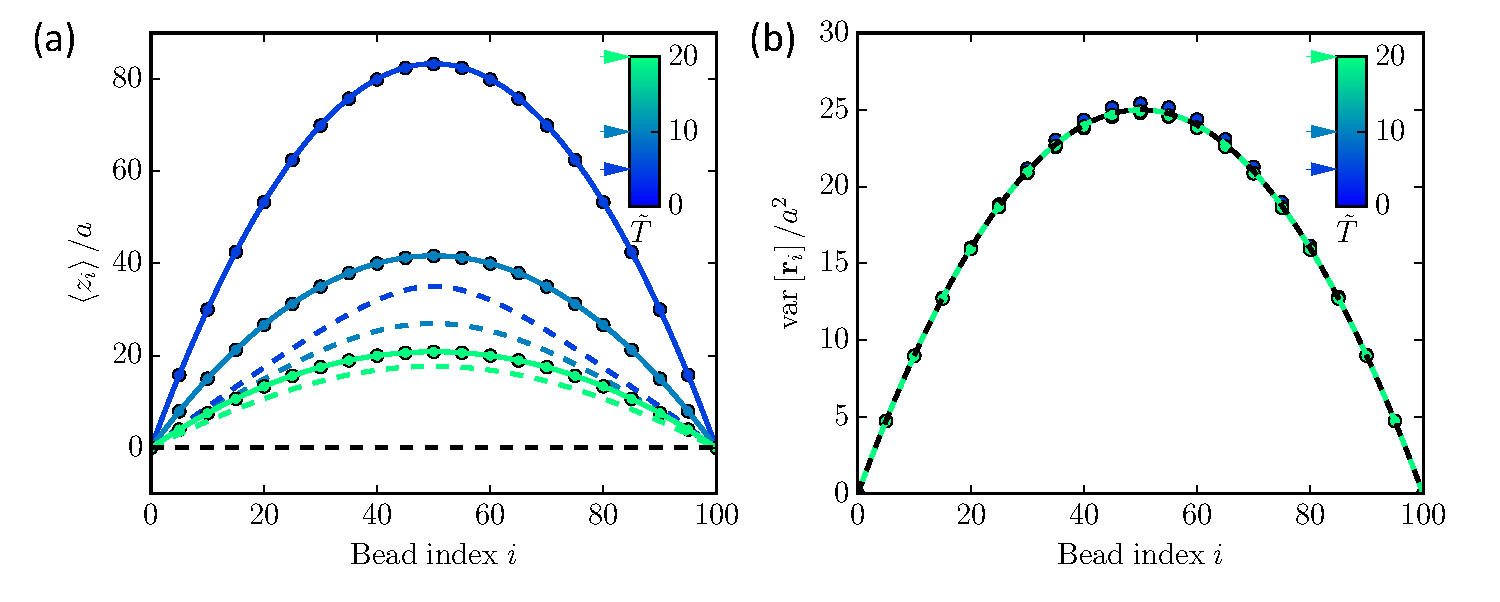
\includegraphics[width=1.0\linewidth]{meanVarRouse}
    \caption{The equilibrium mean and variance of bead position for the bead-spring model, compared with the bead-rod model. (a) Mean bead position of $z$ component. (b) The variance of bead position. Dots are BD simulation results, solid lines are the Rouse theory for the bead-spring polymer loop, dash lines are the theory of the bead-rod model. Different color denotes different dimensionless temperature $\tilde{T}$ which is indicated in the legend. The black dash line in both (a) and (b) shows the force free limit. }
    \label{fig:meanVarRouse}
\end{figure}
We would like to fit the Rouse theory to the bead-rod model if possible. To do this, we take the spring in the bead-spring model as entropic spring and then relate the spring constant to the length of the rod. If the spring in the polymer is the three dimensional entropic spring, then the spring constant can be evaluated by the equipartition theorem as
\begin{equation}
    \label{eq:entropicSpringConstant}
    \frac{1}{2} k_H a^2 = \frac{3}{2} k_B T,
\end{equation}
where $a$ can be interpreted as the equilibrium length of the spring and is set to the length of rod for the comparison. $k_B$ is the Boltzmann constant. So we obtain $k_H = \frac{3k_B T}{a^2}$. Now we can plug it into Eq. \eqref{eq:equilibriumBeadPos} and Eq. \eqref{eq:beadVariance} we arrive at
\begin{subequations}
    \label{eq:beadspringMeanVar}
    \begin{align}
    \left<\mathbf{r}_i^\infty\right> & = 
    \frac{1}{3\tilde{T}}a\mathbf{e}_z \sum_{k=1}^{\frac{L+1}{2}}\frac{\sin\left(\frac{i(2k-1)\pi}{L}\right)} {(2k-1)\pi\sin^2\left(\frac{(2k-1)\pi}{2L}\right)}; \\
    \text{var}\left[\mathbf{r}_i^{\infty}\right] & = a^2\frac{i(L-i)}{L}.
    \end{align}
\end{subequations}
Recalled that $\tilde{T} = k_B T / \Delta E = k_B T / f^e a$. We can now compare the results with the equilibrium results obtained in previous chapter. See in Fig. \ref{fig:meanVarRouse}. Notice that unlike the bead-rod model, the variance of bead position does not depend on the external force field. This is a fundamental difference between the bead-rod and bead-spring model.

For the relaxation time, plug Eq. \eqref{eq:entropicSpringConstant} into the Eq. \eqref{eq:relaxationTimeRouse} and let $L\gg 1$, we obtain
\begin{equation}
    \label{eq:relaxationTimeRouseRod}
    \tau = \frac{\xi a^2 L^2}{3 \pi^2 k_B T}. 
\end{equation}
Interestingly, it is coincide with the relaxation time of a free bead-spring polymer chain with $L$ monomers. And again, it does not depend on the external force field. 

In this section, we discussed the Rouse theory for pinned polymer loop in an external force field. Use the theory we calculate the equilibrium mean and variance of bead position and the relaxation time. The equilibrium results are compared to the results from the bead-rod model. We found the relaxation time of the bead-spring model does not depend on the external force field. Physically, it is caused by the infinite extensibility of the springs and not realistic. To explore to role of finite extensibility, in following sections, we will try to solve the relaxation time of the rigid bead-rod model. In next section, we will first introduce the mapping from the dynamics of pinned polymer loop to ASEP in 1D. 


%********************************** %Second Section  *************************************
\section{1D Pinned Bead-rod Loop Maps to ASEP}
\label{sec:1d_pinned_bead_rod_loop_maps_to_asep}
Like the same strategy used when we study the equilibrium statistics, we also begin with the simplest 1D model for the discussion of dynamics for the pinned bead-rod model. We have illustrated the mapping from one dimensional polymer loop to particles on lattice sites in previous chapter. Here, we will show that the same mapping can also used to study the polymer dynamics. The dynamics of the bead-rod polymer can be mapped to the hopping process of the exclusive particles, which is called ASEP (Asymmetric Simple Exclusion Process). After the illustration of the mapping, we will go back to introduce some of the background knowledge about the ASEP.

\subsection{The mapping to ASEP}
\label{sub:the_mapping_to_asep}
Recall that in the mapping from 1D bead-rod polymer to particle-lattice system, right oriented rods are interpreted as sites occupied by one particle, left oriented rods are interpreted as empty sites. $L$ rods map to exactly $L$ lattice sites, and reflecting boundaries are pertained. The number of particles must be exactly $L/2$ because of the looping condition. 

\begin{figure}[htpb]
    \centering
    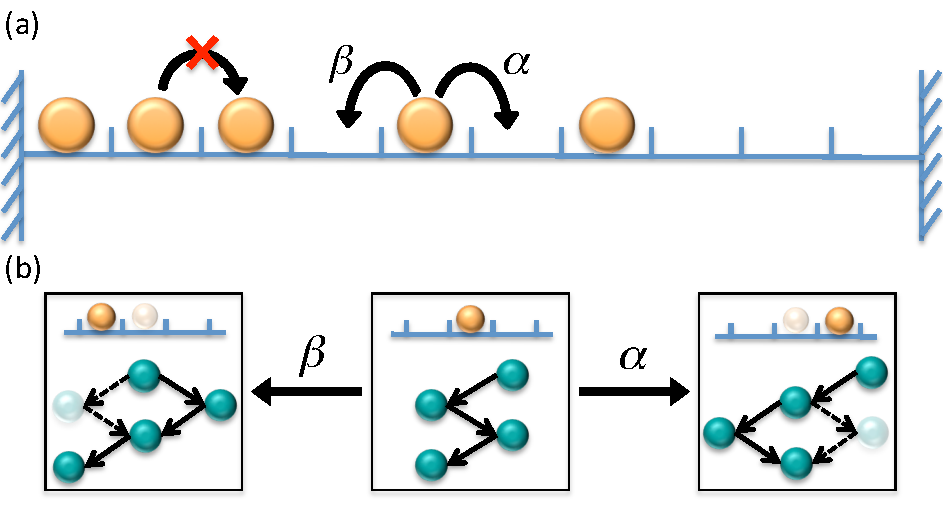
\includegraphics[width=0.8\linewidth]{asep}
    \caption{The schematic of ASEP and the mapping of dynamics. (a) Illustration of ASEP, orange beads represent particle and reflecting boundary is indicated. (b) Illustration of one step particle hopping process maps to the flipping of two neighboring rods in the polymer picture. }
    \label{fig:asep}
\end{figure}

Now, let us consider dynamics problem in the picture of particle-lattice. It is intuitive to imagine the particle can hop to the empty neighboring sites. Multiple occupation is forbidden because the phase space is restricted to be binary. This kind of one dimensional particle hopping process is called Asymmetric Simple Exclusion Process (ASEP). Asymmetric means the hopping rate to left and right is not equal. And the reflecting boundaries can be imposed representing ASEP with reflecting boundary conditions. See in Fig. \ref{fig:asep} (a) for a schematic of the ASEP. Now the question is what is the corresponding process in the polymer picture. 

To answer this question, let us consider just one particle with its neighboring sites and take the example of the particle hops to the left site. The particle hops to the left affects the states of two neighboring sites and thus the states of two neighboring rods in the polymer picture. Correspondingly, the two rods orientation change from left-right to right-left. So one step of particle hopping corresponds to a flip of two neighboring rods in the polymer picture. The same analyse can be applied to the case of particle hops to right. See in the schematic Fig. \ref{fig:asep} (b). And then our next question is how to determine the hopping rate to left and right. 

Let us denote the rate of particle hopping to the right and to the left with $\alpha$ and $\beta$ respectively. Then the detailed balance condition shows
\begin{equation}
    \label{eq:detailedBalance}
    \frac{\alpha}{\beta} = \frac{P_{l+1}}{P_{l}} = \exp\left(-\frac{\Delta E}{k_B T}\right),
\end{equation}
where $P_l$ is the probability of the configuration that $l^{\rm{th}}$ site is occupied while the $(l+1)^{\rm{th}}$ site is not and also represents the corresponding probability of polymer configuration. $\Delta E$ is the energy difference of the two configurations which connects the particle-lattice picture and the polymer picture. And we can obtained from the polymer picture that $\Delta E = 2Fa$ in 1D. On the other hand, the total hopping rate of a particle is determined by the effective temperature of the system, we have 
\begin{equation}
    \label{eq:alphaPlusBeta}
    \alpha + \beta = r_{\text{total}}. 
\end{equation}
Combining Eq. \eqref{eq:detailedBalance} and Eq. \eqref{eq:alphaPlusBeta} we can obtain
\begin{subequations}
    \begin{align}
        \label{eq:hoppingRate}
        \alpha  =   \frac{r_{\text{total}}\exp{(-\Delta E / k_B T)}}{1+\exp{(- \Delta E / k_B T)}}, \\
        \beta  =  \frac{r_{\text{total}}}{1+\exp{(- \Delta E / k_B T)}}.
    \end{align}
\end{subequations}

To determine $r_{\text{total}}$, recall that the hopping of a particle to the neighboring site corresponds to flipping of two rods and thus the displacement of the shared bead by a distance of $2a$. In the case of no external force field, the flipping happens due to the thermal fluctuations. Notice that in the strictly one-dimensional setting, the rods can not continuously turn, there are just initial and final states along or against the field. Therefore, for now we only provide an estimation of the time scale for making a flip, which is the time for a bead to freely diffuse a distance of $2a$. So the total hopping rate can be written as
\begin{equation}
    \label{eq:timeScale}
    r_{\text{total}}^{-1} = \tau_0 = \frac{(2a)^2}{2D} = \frac{2\xi a^2}{k_{B}T}.
\end{equation}
where the diffusion constant $D = k_B/\xi$ is used according to the Einstein relation. 

With Eq. \eqref{eq:hoppingRate} and Eq. \eqref{eq:timeScale}, we know have a well defined ASEP model with reflecting boundary conditions. And we are ready to delve deeper to solve the dynamics. But before that, let us first explain  why do we solve the problem in this way. 

Our goal is to solve the dynamics of the bead-rod polymer in an external force field. However, it is a difficult task as we have shown in previous section that the commonly used Rouse theory does not work. So we use the map from polymer to particle-lattice and define a corresponding ASEP model. The thing is ASEP is one of the fundamental models of non-equilibrium statistical physics with a wealth of tools to analyze it. For example, the Bethe-ansatz method is widely used to solve the model exactly. So our strategy is again to map our essential problem to a well known model and then solve the model and map it back to our original problem. 

Although ASEP is a well studied non-equilibrium model, there are not so many works dealing with the particular case of reflecting boundary conditions. To the best of our knowledge, the exact solution of the full dynamics is still missing. In the next section, we will solve the problem use the Bethe-ansatz method. However, we would like to introduce a little bit the background of ASEP before doing that. 


\subsection{Brief introduction of ASEP}
\label{sub:brief_introduction_of_asep}

ASEP model is said to be a minimal non-equilibrium model similar to the Ising model in equilibrium statistical physics \cite{Derrida1998, Mallick2011b}. Interestingly, it is first proposed for the study of a biological problem. In 1968, MacDonald et al. proposed a mathematical model for the kinetics of protein synthesis by ribosomes, which is essentially the ASEP model \cite{Macdonald1968}. However, the name of ASEP is introduced later in 1970 by Spitzer with the aim of rigorously derive macroscopic hydrodynamic behavior from a microscopic model \cite{Spitzer1970}. The task is done by Varadhan et al. on this specific simple model \cite{hsu1999}. ASEP model has a lot of applications besides those mentioned above. Other examples ranging from the motion of motor molecules along the micro-tubes to the traffic systems \cite{Bressloff2013, schadschneider2010}. 

\begin{figure}[htpb]
    \centering
    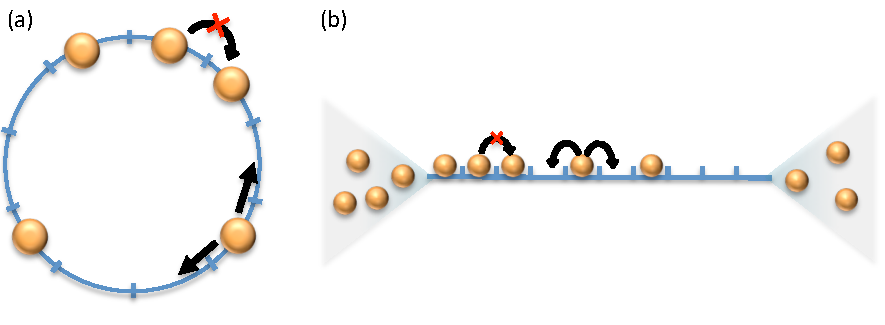
\includegraphics[width=1.0\linewidth]{asepSchematic}
    \caption{Schematics of ASEP model. (a) ASEP with periodic condition. (b) ASEP with open boundary condition.}
    \label{fig:asepSchematic}
\end{figure}

The simplest ASEP model is ASEP with periodic boundaries \cite{Mallick2011b}. See a schematic in Fig. \ref{fig:asepSchematic} (a). The stationary measure is simply a uniform distribution no matter the hopping rates have a bias or not. If there is a bias on the hopping rate, then a steady current will induced in the stationary measure. This is one of the simplest example that detailed balance is not satisfied in the stationary state. The full dynamics of this case can be solved by the Bethe-ansatz method \cite{Batchelor2007}, we will discuss more about it later. 

People are also interested in the case of ASEP on a infinite line from theoretical point of view \cite{Levitt1973,Barkai2010a,Chou2011}. For example, one can derive rigorously the diffusion of a tagged particle for the special case of equal hopping rate to both side.
\begin{equation}
    \label{eq:diffusionInfASEP}
    \left< x^2 \right> = 2 \frac{1-\rho}{\rho}\sqrt{\frac{t}{\pi}},
\end{equation}
where $\rho$ is the density of particles. So we can see it is a sub-diffusion process as long as $\rho\neq 0$. This phenomenon is observed in the experiments \cite{Chou2011}.

ASEP with open boundaries is consider as the minimal microscopic model of transport \cite{Crampe2014b, Mallick2011b}. See in Fig. \ref{fig:asepSchematic} (b). In this model, the two ends of the lattice is connected to two different reservoirs. So the rate of insertion and removal are different at the two ends. For instance, in the simplest case, particles can only be inserted at one end and removed at the other end. So a current can be induced by the bias hopping rates. In 1991, Krug et al. studied the ASEP with open boundaries and discovered the phase transitions in the model. Depends on the insertion or removal rates at the ends, the stationary state of the system can be in high density, low density or maximum current phase. And the phase transition can occur by adjusting those boundary conditions \cite{Krug1991}. 

In order to solve the stationary state of the open ASEP, Derrida et al. proposed an approach which is now called Matrix Product Ansatz. It is a brilliant method far more useful than it though to be at the beginning. Interested readers can refer to the excellent review paper for more details. There is a booming of researches on the topic of ASEP after the work of Derrida and his co-workers. A lot of people make significant contributions to the field. For example, in 1994, Sch\"{u}tz et al. investigate the reflecting ASEP use the $U_q(SU(2))$ quantum group \cite{Sandow1994}. The exact stationary solution was found but not the dynamics. De Gier found the exact solution of open ASEP with certain special constraints in 2005 \cite{DeGier2005}. Spohn et al. constructed an exact solution of the KPZ equation using the ASEP in 2010 \cite{Sasamoto2010}. 

Despite the simplicity of the ASEP model, the way to find the solution of general open ASEP system is still an open question \cite{Crampe2014b, Mallick2011b}. There are a lot of efforts working in this direction. Although the Matrix Product Ansatz is widely used in the study of the stationary state ASEP. The Bethe-ansatz method is more powerful when it comes to the dynamics. We will discuss more about it because we are going to use a generated version of this method to solve the reflecting ASEP in our problem. 

Bethe-ansatz is a method proposed by Hans Bethe in 1931 to solve the Heisenberg spin chain model with periodic condition \cite{Bethe1931}. At that time, he did not realize his great work opened a new branch of physics which is now called the integrability theory \cite{Batchelor2007}. In 1963, Lieb-Liniger use the Bethe-ansatz method solved the Bose gas with $\delta$ interaction potential \cite{Lieb1963a,Lieb1963}. Another important application of Bethe-ansatz is the six vertex model which is also solved by Lieb. The next big step was the discovery of the Yang-Baxter equation, which is introduced independently by C.N. Yang and Rodney Baxter \cite{Yang1967,Baxter1972}. The Yang-Baxter equation provides a criteria to find out whether a model is integrable model or not \cite{Batchelor2007}. The investigation of the Yang-Baxter equation led to the introduction of quantum group theory and the theory of topological knot invariants etc. During 1970s and 1980s, advanced Bethe-ansatz methods like functional Bethe-ansatz  and algebraic Bethe-ansatz were developed \cite{Mallick2011b}. After the introduction of the ASEP model, these Bethe-ansatz methods were quickly adopted to solve it because of the intrinsic connection from ASEP to a spin chain system. For example, the solution of periodic ASEP is almost identical to the Heisenberg spin chain with periodic condition \cite{Mallick2011b}. The study of ASEP and Bethe-ansatz is still a very active field. There are a lot of references one can refer to \cite{Derrida1998,Liggett1999,Schutz2001,Golinelli2006,Mallick2011b}. 

In this section, we introduce the mapping from polymer dynamics to the ASEP model with reflecting boundaries. Moreover, the history of ASEP model and the Bethe-ansatz method are introduced briefly. In next section, we will use the generalized Bethe-ansatz method to solve the reflecting ASEP model. Use the solution, we map it back to understand the polymer dynamics. To the best of knowledge, the exact solution we will present is new and the way of generalization the Bethe-ansatz is novel. We will show it in details. 


%********************************** % Third Section  *************************************
\section{The Bethe-ansatz Solution of ASEP}
\label{sec:the_bethe_ansatz_solution_of_asep}
In this section, we will use the generalized Bethe-ansatz method to solve the dynamics of the ASEP model with reflecting boundaries. The traditional Bethe-ansatz utilize the superposition of plane wave function as the trial solution. In our generalised method, we will show that the solution can be constructed by the combination of single particle eigenfunctions. And the single particle eigenfunction, which takes into account the boundary condition, can be more complex than the simple plane wave functions. So in order to construct the solution, let us first discuss the single particle solution.

\subsection{Solution of single particle}
\label{sub:solution_of_single_particle}
The master equation of a single particle on a closed lattice with $L$ sites can be written as:
\begin{subequations}
    \begin{align}
    \label{eq:single-particle-a}
    \frac{d}{dt} P(x,t) & =  \alpha P(x-1,t) + \beta P(x+1,t) - (\alpha + \beta)P(x,t), \\
    \label{eq:single-particle-b}
    \frac{d}{dt} P(1,t) & =  \beta P(2,t) - \alpha P(1,t),\\
    \label{eq:single-particle-c}
    \frac{d}{dt} P(L,t) & =  \alpha P(L-1,t) - \beta P(L,t),
    \end{align}
\end{subequations}
where $\alpha$ and $\beta$ is hopping rate of particle to left and right, respectively. See in the schematic Fig. \ref{fig:asep} (a). $P(x,t)$ is the probability of a particle sitting on site $x$ at time $t$, and $x$ is confined to be the integer in the range of $x\in\{1,2,\cdots,L\}$. Eq.  \eqref{eq:single-particle-b} and \eqref{eq:single-particle-c} are actually the special cases of master equation at the boundaries.  It is much more convenient to rewrite Eq. \eqref{eq:single-particle-b} and \eqref{eq:single-particle-c} as the following boundary conditions:
\begin{subequations}
    \label{eq:boundaries-single-particle}
    \begin{align}
        \label{eq:boundaries-single-particle-a}
        \alpha P(0,t) = \beta P(1,t),\\
        \label{eq:boundaries-single-particle-b}
        \alpha P(L,t) = \beta P(L+1,t).
    \end{align}
\end{subequations}
The notation above might look confusing. Because $x=0,L+1$ are sites out of the domain and one would expect the corresponding $P(x,t)=0$. However, this notation actually employs a technique called ``ghost coordinate", which is often used in the analysis of stochastic processes. To clarify the concept, we remark several points here:

$\bullet$ By writing down Eq. \eqref{eq:boundaries-single-particle}, we actually introduced an auxiliary space with infinite lattice sites where only the master equation Eq. \eqref{eq:single-particle-a} is satisfied. So in the auxiliary space, $P(0,t)$ and $P(L+1,t)$ are not necessary vanished.

$\bullet$ Based on the auxiliary space, we then impose additional constraints. Eq. \eqref{eq:boundaries-single-particle-a} can be interpreted as the flux from site $0$ going right to site $1$ equals to the flux from site $1$ going left to site $0$. Similarly, the same interpretation can also be applied to Eq. \eqref{eq:boundaries-single-particle-b}. So the boundary condition simply means the net flux at the boundaries are vanished. Namely, the reflecting boundary condition is imposed. 

$\bullet$ Physically, the real PDF $P(x,t)$ is normalized in the domain $x\in\{1, 2, \cdots, L\}$, and the probability outside the domain is zero.

$\bullet$ Mathematically, Eq. \eqref{eq:boundaries-single-particle} can be derived simplicity by assuming Eq. \eqref{eq:single-particle-a} is valid in the whole space and do a subtraction of Eq. \eqref{eq:single-particle-a} to Eq. \eqref{eq:single-particle-b} and Eq. \eqref{eq:single-particle-a} to Eq. \eqref{eq:single-particle-c}, respectively.  

Now, our governing equations are the master equation Eq. \eqref{eq:single-particle-a} and boundary conditions Eq. \eqref{eq:boundaries-single-particle}. To solve these equations, let us take the ansatz of separation of variables $P(x,t) = \phi(x)e^{\lambda t}$ and plug into the master equation, obtaining 
\begin{equation}
    \label{eq:eigen}
    \beta\phi(x+1) -(\alpha+\beta+\lambda)\phi(x) + \alpha\phi(x-1) = 0.
\end{equation}
Given that $x$ is an integer number, Eq. \eqref{eq:eigen} is essentially a set of liner difference equations. Substituting the ansatz of $P_x(t)$ into boundaries of Eq. \eqref{eq:boundaries-single-particle}, we obtain
\begin{subequations}
    \label{eq:boundaries-phi}
    \begin{align}
        \alpha\phi(0) &= \beta\phi(1), \\
        \alpha \phi(L) &= \beta \phi(L+1).
    \end{align}
\end{subequations}
The standard method to find the solution is to take an ansatz $\phi(x) = Az^x$, where $z$ is an arbitrary complex number. We arrive at the characteristic quadratic equation:
\begin{equation}
    \label{eq:characteristic}
    \beta z^2 - (\alpha + \beta + \lambda ) z + \alpha = 0.
\end{equation}
The two roots fulfill $z_+z_- = \frac{\alpha}{\beta}$. And the solution of \eqref{eq:eigen} can be written as 
\begin{equation}
    \label{eq:eigen-solution}
    \phi(x) = A_+ z_+^{x} + A_- z_-^{x}
\end{equation}
By applying the boundaries Eq. \eqref{eq:boundaries-phi} to Eq. \eqref{eq:eigen-solution} we can find all the eigenvalues and corresponding eigenvectors. The results are summarised as following. The stationary eigenmode with zero eigenvalue is
\begin{subequations}
    \label{eq:single-particle-stationary}
    \begin{align}
        \phi_s(x) & = const. \left(\frac{\alpha}{\beta}\right)^{x}, \\
        \lambda_s & = 0. 
    \end{align}
\end{subequations}
There are $L-1$ non-stationary eigenmodes and corresponding eigenvalues, which can be written as
\begin{subequations}
    \label{eq:single-particle-eigenmodes}
    \begin{align}
        \phi_k(x) & = const. \left(\frac{\alpha}{\beta}\right)^{\frac{x}{2}} \left[\sin\left(\frac{k\pi}{L}x\right) - \sqrt{\frac{\beta}{\alpha}}\sin\left(\frac{k\pi}{L}(x-1)\right)\right],\\
        \lambda_k & = -(\alpha+\beta) + 2\sqrt{\alpha\beta}\cos(\frac{k\pi}{L}); ~k=1,2,\dots, L-1.
    \end{align}
\end{subequations}

The eigenvalue $\lambda_s = 0$ and corresponding eigenvector represent the stationary mode $\phi_s(x)$. Define a scalar product between any two functions by 
\begin{equation}
    \label{eq:scalarPoduct} (\phi, \psi) =
    % \int\frac{\phi(x)\phi(x)}{\phi_{0}(x)}dx 
    \sum_{x}\frac{\phi(x)\psi(x)}{\phi_{s}(x)}
\end{equation}
Notice that definition Eq. \eqref{eq:scalarPoduct} makes $\phi_s(x)$ identical to the stationary distribution $P^e(x)$, and remember here $x$ is an integer. By properly choose the constant and when $L\rightarrow\infty$, one can check the orthogonality and completeness of the eigenfunctions.
\begin{subequations}
    \begin{align}
        \label{eq:orthogonality}
        \sum_{x=1}^L \phi_k(x)\phi_l(x) & = \delta_{k,l}, \\
        \label{eq:completeness}
        \sum_{k=1}^L \phi_k(x)\phi_k(y) & = \delta_{x,y}.
    \end{align}
\end{subequations}
So for an arbitrary initial distribution of $P(x, 0)$, we can always decompose it as 
\begin{equation}
    \label{eq:decompose-intial-single}
    P(x,0) = \sum_k{c_k \phi_k(x)},
\end{equation}
where $c_k$ can be calculated by 
\begin{equation}
    \label{eq:coeff-k}
    c_k = \sum_x{\phi_k(x) P(x,0)}.
\end{equation}
Finally, the solution of single particle on reflecting lattice can be written as
\begin{equation}
    \label{eq:solution-single}
    P(x,t) = \sum_k{\phi_k(x)e^{\lambda_k t}}\sum_{x^\prime}{\phi_k(x^\prime)P(x^\prime,0)}.
\end{equation}
For the special case that $P(x,0) = \delta_{x,y}$, solution \eqref{eq:solution-single} can be simplified to
\begin{equation}
    \label{eq:solution-single-simplified}
    P(x,t) = \sum_k{\phi_k(x)\phi_k(y)e^{\lambda_k t}}
\end{equation}

With the complete solution of single particle, we can go further to systems of more than one particle. The idea is that the single particle solution works as building blocks for the $N$ particle solutions. To start with that, we first illustrate the case $N=2$ and the position of particles are denotes by $x_1, x_2$ with the constraint $x_1<x_2$.

\subsection{Solution of two particles}
\label{sub:solution_of_two_particles}
Denote $P(x_1,x_2;t)$ the probability of the two particles sitting at $x_1$ and $x_2$ respectively at time $t$. Firstly, we shall write down the master equation, which looks as following
\begin{equation}
    \begin{aligned}
    \label{eq:masterEqTwo}
    \frac{d P(x_1, x_2; t)}{dt} = & \alpha P(x_1-1,x_2;t) + \beta P(x_1+1,x_2;t) \\ 
    & + \alpha P(x_1, x_2-1; t) + \beta P(x_1, x_2+1; t)  \\ 
    & - 2(\alpha+\beta)P(x_1, x_2; t)
    \end{aligned}
\end{equation}
We take the same eigenfunction expansion as for the single particle case:
\begin{equation}
    \label{eq:solutionTwo}
    P(x_1, x_2, t) = \sum_{k} \Psi_{k}(x_1, x_2) e^{\Lambda_k t}
\end{equation}
Plug it into the master equation Eq. \eqref{eq:masterEqTwo} we have
\begin{equation}
    \begin{aligned}
    \label{eq:eigenModesTwo}
    \Lambda \Psi(x_1, x_2) = & \alpha \Psi(x_1-1, x_2) + \beta \Psi(x_1+1, x_2)
    \\ &+ \alpha \Psi(x_1, x_2-1) + \beta \Psi(x_1, x_2+1) \\ 
    &- 2(\alpha+\beta)\Psi(x_1, x_2)
    \end{aligned}
\end{equation}
And the reflecting boundaries write as
\begin{subequations}
    \label{eq:boundaries-two-particles}
    \begin{align}
        \alpha \Psi(0,x_2) = \beta \Psi(1, x_2) \\
        \alpha \Psi(x_1, L) = \beta \Psi(x_1, L+1)
    \end{align}
\end{subequations}
For the case of more than one particle, we need to take into account the exclusion effect, i.e., one site can be occupied by at most one particle. This can be also written as a boundary condition as 
\begin{equation}
    \label{eq:exclusionCondition}
    \alpha \Psi(x, x) + \beta \Psi(x+1, x+1) = (\alpha + \beta) \Psi(x, x+1)
\end{equation}
Notice that the exclusive condition must hold for any $x$. The notation of $\Psi(x, x)$ may looks a little bit weird, but keep in mind that it is a boundary condition that denotes the limiting situation $x_1=x_2$. And we can understand it in the same way of understanding the ``ghost coordinate" in the single particle case. See in appendix \ref{} for a detailed derivation of Eq. \eqref{eq:exclusionCondition}. 

Before delve into the Bethe Ansatz solution, let us release the fixed coefficients of eigenfunctions in Eq. \eqref{eq:single-particle-stationary} and Eq. \eqref{eq:single-particle-eigenmodes}, rewrite them as the following general form:
\begin{subequations}
    \label{eq:eigenModes}
\begin{align}
    \label{eq:stationaryEigenMode}
    \psi_s(x)  & =  A\left(\frac{\alpha}{\beta}\right)^x, \\
    \label{eq:nonstationaryEigenModes}
    \psi_{ns}(x) & =  \left(\frac{\alpha}{\beta}\right)^{\frac{x}{2}} \left(A_+ e^{ipx} +  A_-e^{-ipx}\right),
\end{align}
\end{subequations}
where $\psi_s$ and $\psi_{ns}$ represent stationary eigenfunction and non-stationary eigenfunctions respectively, $A,~A_+,~A_-$ are amplitude coefficients, $p$ is the wave vector of excited eigenmodes. In case of single particle case above, these coefficients can be fixed by applying the boundary conditions Eq. \eqref{eq:boundaries-single-particle}. Here however, we will leave them free now and use the general form to construct the Bethe-ansatz solution. Boundary conditions will be imposed afterwards and all unfixed coefficients can be solved by then. 

The idea to construct the $N$ particle solution is inspired by the standard Coordinate Bethe Ansatz (CBA). However, instead of using the plain plane wave function as building blocks, we use the general form of single particle eigenfunctions with unfixed coefficients. The example of ansatz for $\Psi(x_1, x_2)$ reads
\begin{equation}
    \label{eq:ansatzTwo}
    \Psi(x_1, x_2) = \psi_1(x_1)\psi_2(x_2) + \tilde{\psi}_2(x_1)\tilde{\psi}_1(x_2).
\end{equation}
Here $\psi_n(x)$ and $\tilde{\psi}_n(x)$ are functions draw from of Eq. \eqref{eq:eigenModes}, either stationary Eq. \eqref{eq:stationaryEigenMode} or non-stationary Eq.\eqref{eq:nonstationaryEigenModes}. There are two particles in the system thus we have the index $n$ in the range of $n=1,2$. 
We classify $\psi_1, ~\tilde{\psi}_1$ as one class and $\psi_2,~\tilde{\psi}_2$ as the other class. Functions in the same class (e.g. $\psi_1$ and $\tilde{\psi}_1$) share the same wave vector ($p_1=\tilde{p}_1$), but different amplitude coefficients ($A_{1\pm}\neq \tilde{A}_{1\pm}$). If this class is draw from the stationary mode Eq. \eqref{eq:stationaryEigenMode}, then simply the functions in the class ($\psi_1$ and $\tilde{\psi}_1$) are only differentiated by amplitude coefficient ($A_1\neq\tilde{A}_1$). 
It is important that $\psi_n$ and $\tilde{\psi}_n$ have different amplitude coefficients. The main idea is to tune these amplitude coefficients so that $\Psi(x_1, x_2)$ satisfies the reflecting boundaries Eq. \eqref{eq:boundaries-two-particles} and exclusive condition Eq. \eqref{eq:exclusionCondition}.  

With the constructed ansatz Eq. \eqref{eq:ansatzTwo}, our remaining task is to impose the constraints Eq. \eqref{eq:boundaries-two-particles} and Eq. \eqref{eq:exclusionConditionTwo} and fix those amplitude coefficients as well as the wave vectors. There are three types of $\Psi(x_1,x_2)$ depending on the combination of the two constructed classes: both stationary, both non-stationary and the mixed type with one stationary and the other non-stationary. In the following subsections, we will discuss these cases separately.  

\subsubsection{Both stationary}
\label{ssub:Both stationary}

Let us first check the case that $\Psi(x_1, x_2)$ are constructed all by stationary eigenmodes. 
Namely $ \psi_1(x) = A_1\left(\frac{\alpha}{\beta}\right)^x, ~\psi_2(x) = A_2\left(\frac{\alpha}{\beta}\right)^x, ~\tilde{\psi}_1(x) = \tilde{A}_1\left(\frac{\alpha}{\beta}\right)^x, ~\tilde{\psi}_2(x) = \tilde{A}_2\left(\frac{\alpha}{\beta}\right)^x$. 
Plug in to \eqref{eq:ansatzTwo} we obtain
\begin{equation}
    \label{eq:stationaryTwo}
    P^e(x_1, x_2) = \Psi(x_1, x_2) = 
    A \left(\frac{\alpha}{\beta}\right)^{x_1+x_2}
\end{equation}
where $A=A_1\tilde{A}_1+A_2\tilde{A}_2$. One can readily check that Eq. \eqref{eq:stationaryTwo} is exactly the stationary eigenfunction of the two particle system as expected. First, we can easily obtain the corresponding eigenvalue is $\Lambda_s=0$ by simply plug it in to Eq. \eqref{eq:eigenModesTwo}.  And then one can check the reflecting boundaries Eq.  \eqref{eq:boundaries-two-particles} and the exclusive condition Eq.  \eqref{eq:exclusionCondition} are both fulfilled. 

The prefactor $A$ can be fixed by normalization. However, it is not a trivial work because of the constraint $x_1 < x_2$. We will discuss in detail in the general case of $N$ particles later. 


\subsubsection{Both non-stationary}
\label{ssub:Both non-stationary}

For a simple two particles system, there are two different types of non-stationary modes. The first type is constructed by one class of Eq.  \eqref{eq:stationaryEigenMode} and one class of Eq.  \eqref{eq:nonstationaryEigenModes}. The second type is constructed all by two classes of Eq. \eqref{eq:nonstationaryEigenModes} with different $p$.

Let us start with the first type. Without loss of generality, we choose
$\{\psi_1(x), \tilde{\psi}_1(x)\}$ to be the class characterized by Eq.
\eqref{eq:stationaryEigenMode}, then $\Psi(x_1, x_2)$ can be written as
\begin{equation}
    \begin{aligned}
        \label{eq:nonstationaryModesTwo1}
        \Psi(x_1, x_2) = & A_{1}\left(\frac{\alpha}{\beta}\right)^{x_1} 
        \left(\frac{\alpha}{\beta}\right)^{\frac{x_2}{2}} \left( A_{2+} 
            e^{ip_2 x_2} + A_{2-} e^{-ip_2 x_2}\right) \\
        & + \tilde{A}_{1}\left(\frac{\alpha}{\beta}\right)^{x_2} \left(
            \frac{\alpha}{\beta}\right)^{\frac{x_1}{2}} \left( \tilde{A}_{2+}
            e^{ip_2 x_1} + \tilde{A}_{2-} e^{-ip_2 x_1}\right) 
    \end{aligned}
\end{equation}
Plug Eq. \eqref{eq:nonstationaryModesTwo1} in to the master equation, we will
find the corresponding eigenvalue. Plug it in to the reflecting boundaries and
exclusive condition, $A_{1},~\tilde{A}_{1},~A_{2\pm}$ and $\tilde{A}_{2\pm}$ can
be tuned to fulfill these conditions. Consistency condition will give us the
Bethe equation about wave vector $p_2$, we will show the details of this
procedure in the following text.

We first insert the solution to the master equation Eq. \eqref{eq:eigenModesTwo},
obtaining the corresponding eigenvalue:
\begin{equation}
    \label{eq:eigenvaluesTwo1}
    \Lambda = -(\alpha+\beta) + 2\sqrt{\alpha\beta}\cos(p_2)
\end{equation} 
$p_2$ is the wave vector that will be determined later. 

Accordingly, the reflecting condition Eq. \eqref{eq:boundaries-two-particles}
gives us
\begin{subequations}
    \label{eq:scatterFactorBoundary}
    \begin{align}
        \frac{A_{2+}}{A_{2-}} & = & -\frac{\left(\alpha-\sqrt{\alpha\beta}
                e^{-ip_2}\right) e^{-ip_2L}}{\left(\alpha-\sqrt{\alpha\beta} 
                e^{ip_2}\right) e^{ip_2L}}  \\
        \frac{\tilde{A}_{2+}}{\tilde{A}_{2-}} & = & -\frac{\alpha -
            \sqrt{\alpha\beta} e^{-ip_2}}{\alpha-\sqrt{\alpha\beta} e^{ip_2}} 
    \end{align}
\end{subequations}

We now check the exclusive condition Eq. \eqref{eq:exclusionCondition}. Simply
substitute Eq.  \eqref{eq:nonstationaryModesTwo1} into the condition. In order to
fulfill the exclusive condition, we find that 
\begin{subequations}
    \label{eq:scatterFactorExclusive}
    \begin{align}
        \frac{A_{1}A_{2+}}{\tilde{A}_{1}\tilde{A}_{2+}} & = & -\frac{\alpha
            e^{ip_2}-(\alpha+\beta) \sqrt{\frac{\alpha}{\beta}} +
            \sqrt{\alpha\beta} }{\alpha e^{ip_2} -(\alpha+\beta)e^{ip_2} +
            \sqrt{\alpha\beta} } \\
        \frac{A_{1}A_{2-}}{\tilde{A}_{1}\tilde{A}_{2-}} & = & -\frac{\alpha
            e^{-ip_2}-(\alpha+\beta) \sqrt{\frac{\alpha}{\beta}} +
            \sqrt{\alpha\beta} }{\alpha e^{-ip_2} -(\alpha+\beta)e^{-ip_2} +
            \sqrt{\alpha\beta} } 
    \end{align}
\end{subequations}
Finally, use the consistency condition that
\begin{equation}
    \label{eq:consistencyConditionTwo}
    \frac{\tilde{A}_{2+}}{\tilde{A}_{2-}}\frac{A_{2-}}{A_{2+}} = 
    \frac{\tilde{A}_{1}\tilde{A}_{2+}}{A_{1}A_{2+}}
    \frac{A_{1}A_{2-}}{\tilde{A}_{1}\tilde{A}_{2-}}
\end{equation}
We obtain the Bethe equation 
\begin{equation}
    \label{eq:betheEqTwo1}
    e^{i2p_2L} = 1
\end{equation}
Solve the equation we get $p_2=\frac{k\pi}{L}$. Notice that it is exactly the
same as the spectrum of single particle case. With the solution of $p_2$ we can
resubstitute it into Eq. \eqref{eq:scatterFactorBoundary} and Eq.
\eqref{eq:scatterFactorExclusive} to get the corresponding eigenfunctions. 
The results of this type of non-stationary eigenvalues and corresponding
eigenfunctions are summarized as following 
\begin{subequations}
    \label{eq:eigenTwo}
    \begin{align}
        \label{eq:eigenvaluesTwo}
        \Lambda_k & = &
        -(\alpha+\beta) + 2\sqrt{\alpha\beta}\cos(\frac{k\pi}{L});
        ~k=1,2,\dots, L-1  \\
        \label{eq:eigenvectorsTwo}
        \Psi_k(x_1, x_2) & = & A\left[ \frac{\alpha}{\beta}
            \left(\frac{\alpha}{\beta}
            \right)^{x_1}\phi_k(x_2)+\left(\frac{\alpha}{\beta}\right)^{x_2}
            \phi_k(x_1) \right]
    \end{align}
\end{subequations}
Here $\phi_k(x)$ is exactly single particle non-stationary eigenfunction and
$A$ is a constant normalization coefficient.

We now turn to the second type of non-stationary eigenmodes. Notice that, the
number of remaining unknown eigenfunctions and eigenvalues is in principle
$L(L-1)/2 - L$. We will show that there are all contained in this class. We
first write down the Ansatz:
\begin{equation}
    \label{eq:nonstationaryModesTwo2}
    \begin{aligned}
        \Psi(x_1, x_2) = &  \left(\frac{\alpha}{\beta}\right)^{\frac{x_1+x_2}{2}} 
        \left[\left( A_{1+} e^{ip_1 x_1} + A_{1-} e^{-ip_1 x_1}\right)  
            \left( A_{2+} e^{ip_2 x_2} + A_{2-} e^{-ip_2 x_2}\right) \right.\\
        & \left. + \left( \tilde{A}_{1+} e^{ip_1 x_2} + \tilde{A}_{1-} e^{-ip_1
                    x_2}\right)  \left( \tilde{A}_{2+} e^{ip_1 x_1} +
                \tilde{A}_{2-} e^{-ip_2 x_1}\right) \right]
    \end{aligned}
\end{equation}
Plug it in to the master equation, we get the corresponding eigenvalues
\begin{equation}
    \label{eq:eigenvaluesTwo2}
    \Lambda = \sum_{n=1}^2\left[-(\alpha+\beta) + 
        2\sqrt{\alpha\beta}\cos(p_n)\right]
\end{equation} 
And plug it in to the reflecting boundaries, we obtain
\begin{subequations}
    \label{eq:scatterFactorBoundary2}
    \begin{align}
        \frac{A_{1+}}{A_{1-}} & = & -\frac{\alpha-\sqrt{\alpha\beta}
                e^{-ip_1}}{\alpha-\sqrt{\alpha\beta} e^{ip_1}}  \\
        \frac{\tilde{A}_{1+}}{\tilde{A}_{1-}} & = & 
        -\frac{\left(\alpha-\sqrt{\alpha\beta} e^{-ip_1}\right) e^{-ip_1L}}
        {\left(\alpha-\sqrt{\alpha\beta} e^{ip_1}\right) e^{ip_1L}}  \\
        \frac{\tilde{A}_{2+}}{\tilde{A}_{2-}} & = & -\frac{\alpha -
            \sqrt{\alpha\beta} e^{-ip_2}}{\alpha-\sqrt{\alpha\beta} e^{ip_2}}\\
        \frac{A_{2+}}{A_{2-}} & = & -\frac{\left(\alpha-\sqrt{\alpha\beta}
                e^{-ip_2}\right) e^{-ip_2L}}{\left(\alpha-\sqrt{\alpha\beta} 
                e^{ip_2}\right) e^{ip_2L}}
    \end{align}
\end{subequations}
To ease the notation, we define the function $a(p, p^\prime) =
\sqrt{\alpha\beta}e^{i(p+p^\prime)}-(\alpha+\beta)e^{ip}+\sqrt{\alpha\beta}$.
Then the exclusive condition gives 
\begin{subequations}
    \label{eq:scatterFactorExclusive2}
    \begin{align}
        \frac{A_{1+}A_{2+}}{\tilde{A}_{1+}\tilde{A}_{2+}} & = & 
        -\frac{a(p_1, p_2)}{a(p_2, p_1)} \\
        \frac{A_{1+}A_{2-}}{\tilde{A}_{1+}\tilde{A}_{2-}} & = & 
        -\frac{a(p_1, -p_2)}{a(-p_2, p_1)} \\
        \frac{A_{1-}A_{2+}}{\tilde{A}_{1-}\tilde{A}_{2+}} & = & 
        -\frac{a(-p_1, p_2)}{a(p_2, -p_1)} \\
        \frac{A_{1-}A_{2-}}{\tilde{A}_{1-}\tilde{A}_{2-}} & = & 
        -\frac{a(-p_1, -p_2)}{a(-p_2, -p_1)}
    \end{align}
\end{subequations}
The similar consistency condition of Eq. \eqref{eq:consistencyConditionTwo}
gives the following Bethe equation:
\begin{subequations}
    \label{eq:betheEqTwo2}
    \begin{align}
        e^{i2p_1L} & = & \frac{a(p_1, p_2)}{a(p_2, p_1)} 
        \frac{a(p_2, -p_1)}{a(-p_1, p_2)}\\
        e^{i2p_2L} & = & \frac{a(p_2, p_1)}{a(p_1, p_2)} 
        \frac{a(p_1, -p_2)}{a(-p_2, p_1)}
    \end{align}
\end{subequations}
Now it would be interesting to interpret the Bethe Equation and compare with
the well know Bethe Equation of priodic boundary case. And we will show later
this interpretation is useful to derive $N$ particles Bethe Equation. We can
consider Eq.  \eqref{eq:scatterFactorBoundary} as a reflector that reflects the
particle and change the direction of wave vector, i.e., $p_n\leftrightarrow-p_n$.
On the other hand, Eq. \eqref{eq:scatterFactorExclusive} can be interpreted as
a permutator that permutates two neighboring particles $n\leftrightarrow (n+1)$.
Let us say particle $1$ starts from the left side of the lattice and then
permutates with all the particle at right side until reaches the right boundary
(of course in case of two particles, there are only one particle at the right
side), and then reflects by the boundary, become a particle traveling in the
oppsite direction, and then permutates with all the left side particles until
reaches the left side boundary, and then reflects again, which recovers the
initial state. A schematic of this process is shown in Fig.
\ref{fig:betheEq}. In this sense, the particle works as if it is on a
lattice with periodic boundary. Use this interpretation and the well know result
of periodic Bethe Equation, once can easily recover exactly Eq.
\eqref{eq:betheEqTwo2}. 

% \begin{figure}[htpb]
%     \centering
%     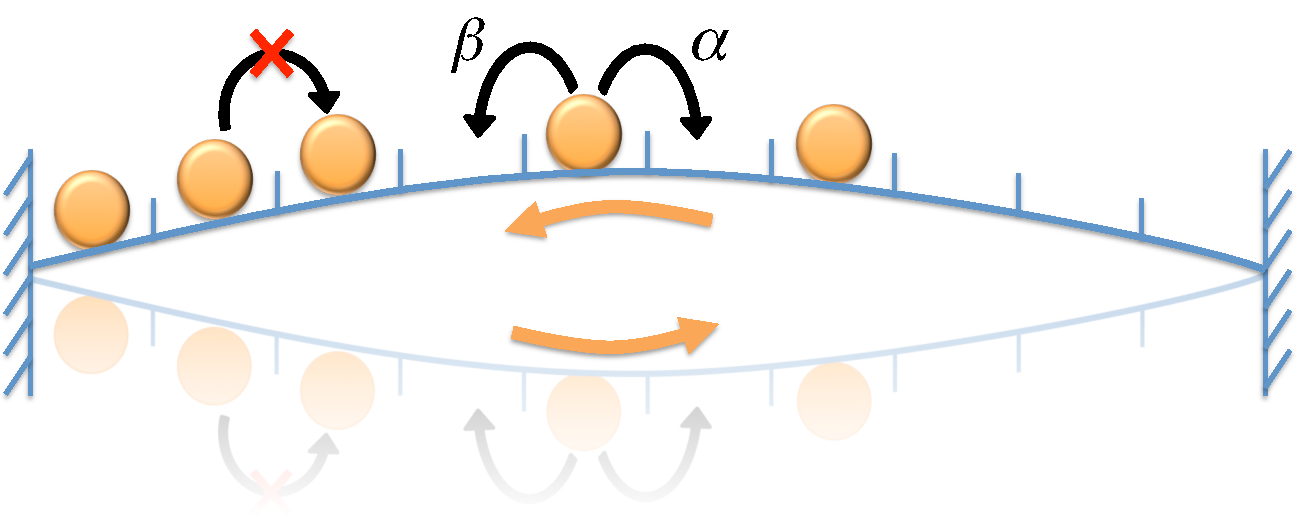
\includegraphics[width=0.8\linewidth]{betheEq}
%     \caption{Intepretation of Bethe Equation.}
%     \label{fig:betheEq}
% \end{figure}
By solving the Bethe equation, one can get $p_1$ and $p_2$ and thus all
amplitude coefficients up to a constant normalization factor. Then Eq.
\eqref{eq:eigenvaluesTwo2} gives the eigenvalues and Eq.
\eqref{eq:nonstationaryModesTwo2} gives the eigenfunctions.
Unfortunately, it might not possible to solve the Bethe equation analytically.
So we resort to numerical solutions. We have verified the resulting eigenvalues
and eigenfunctions by benchmark with the results from brute force diagonalizing
of the transition matrix for small system size $L\le10$. Notice that those roots
that $p_n=0$ or $p_n=\pi$ have to be filtered out because they correspond to the
first type of non-stationary eigenmodes which is not compatible by Eq.
\eqref{eq:nonstationaryModesTwo2}


To summarize, the complete solution of two particle hopping system with
reflecting boundaries was found. The solution is shown in the form of
eigenfunction expansion, i.e. Eq. \eqref{eq:eigenModesTwo}. The stationary
eigenfunction with eigenvalue $\Lambda_0=0$ is listed as Eq.
\eqref{eq:stationaryTwo}, while the two types of non-stationary eigenvalues and
corresponding eigenfunctions are listed in Eq. \eqref{eq:eigenvaluesTwo1},
\eqref{eq:eigenvaluesTwo2} and Eq.
\eqref{eq:nonstationaryModesTwo1}, \eqref{eq:nonstationaryModesTwo2},
respectively. They can be fully determined by  solving the Bethe Equation Eq.
\eqref{eq:betheEqTwo1} and Eq. \eqref{eq:betheEqTwo2}. Part of them are
analytically shown in Eq. \eqref{eq:eigenTwo}.

Finally, there are several remarks we want to make here.
Firstly, as one can see from Eq.  \eqref{eq:eigenTwo} that the eigenvalues of two
particle system always contain the eigenvalues of single partile system. We will
show later this can be generalised that the eigenvalues of $N+1$ particle system
always contain the eigenvalues of $N$ particle system for $N<L/2$. Secondly, the
relaxation time of the system is realted to the largest non-zero eigenvalue
$\Lambda_1$. Eq.  \eqref{eq:eigenTwo} hints
$\Lambda_1=-(\alpha+\beta)+2\sqrt{\alpha\beta} \cos\left(\frac{\pi}{L}\right)$.
However, since there is no analytical solution for eigenvalues of the second
kind, it will be difficult to rigously prove that. Nummerical evidences will be
provided to verify this is indeed true.

In next section, we will generalise the solution to the $N$ particles system.
It is actually quite straight forward after we have done the two particles
case. 


\section{General Solution of $N$ particles ASEP}
\label{sec:general_solution_of_n_particles_asep}

As before, we first write down the master equation of a $N$ particles system.
\begin{equation}
    \begin{aligned}
        \label{eq:masterEqN}
        \frac{d P(x_1, \cdots, x_N; t)}{dt} = & \sum_{j=1}^N \left[\alpha
            P(\cdots,x_j-1,\cdots;t) + \beta P(\cdots, x_j+1, \cdots;t)\right. \\ 
        & \left.- (\alpha+\beta)P(\cdots, x_j, \cdots; t)\right]
    \end{aligned}
\end{equation}

Similarly, after the eigenfunction expansion the reflecting boundaries write as
\begin{subequations}
    \label{eq:boundaries-N-particles}
    \begin{align}
        \alpha \Psi(0,x_2,\cdots,x_N) = \beta \Psi(1, x_2,\cdots, x_N) \\
        \alpha \Psi(x_1,\cdots, x_{N-1}, L) = \beta \Psi(x_1,\cdots, x_{N-1}, L+1)
    \end{align}
\end{subequations}
The exclusive condition for $N$ particles case is more tricky. In principle,
one has to consider to case of three body collision and four body collision and
so on. Luckily, in the simple model of ASEP, one can prove that these more than
two body exclusive conditions are not new but just linear recombination of two
body exclusive condition. So we can write the exclusive condition of a $N$
particles system as 
\begin{equation}
    \label{eq:exclusionConditionN}
    \alpha \Psi(\cdots,x, x,\cdots) + \beta \Psi(\cdots, x+1, x+1, \cdots) 
    = (\alpha + \beta) \Psi(\cdots, x, x+1, \cdots)
\end{equation}
The reason that the exclusive condition can be written in such a simple way is
rooting from the Yang-Baxter Equation, which encodes the integrability of the
ASEP system.

\subsection{Stationary Solution}
\label{sub:stationary_solution}

Intuitively, we construct the $N$ particles stationary solution as
\begin{equation}
    \label{eq:stationaryN}
    P^e(x_1, x_2, \cdots, x_N) = \Psi(x_1, x_2, \cdots, x_N) =  A
    \prod_{j=1}^N\left(\frac{\alpha}{\beta}\right)^{x_j}
\end{equation}

One can plug in the master equation check that the corresponding eigenvalue
$\Lambda_0= 0$, and also verify the exclusive condition as well as the reflecting
boundaries are fulfilled by insert the solution in to Eq.
\eqref{eq:exclusionConditionN} and Eq. \eqref{eq:boundaries-N-particles}
separately.

We now try to fix the parameter $A$ by normalization. Let us denote
$q:=\frac{\alpha}{\beta}$, then we can write $A$ as following
\begin{equation}
    \label{eq:stationaryPrefactor}
    A^{-1} = \sum_{\Omega} q^{\sum_j{x_j}} = 
    \sum_{x_1 < x_2 < \cdots < x_N} q^{\sum_j{x_j}}
\end{equation}
Let us do a variable change so that 
\begin{align*}
    \sum_j{x_j} &=& E_0 + E \\
    E_0 &=& 1 + 2 + \cdots + N = \frac{N(N+1)}{2}
\end{align*}
We can derive that $E$ is a integer in the range of $0, 1, \cdots, N(L-N)$. So
Eq. \eqref{eq:stationaryPrefactor} can be rewrite as 
\begin{equation}
    \label{eq:prefactorRewrite}
    A^{-1} = q^{E_0}\sum_{E=0}^{N(L-N)}g(E)q^E
\end{equation}
where $g(E)$ is the number of partitions of positive integer $E$ to $N$ parts
with each of size at most $L-N$. From the number partition theory, we identify
\begin{equation}
    \label{eq:degeneratcy}
    \sum_{E=0}^{N(L-N)}g(E)q^E = \binom{L}{N}_q =
    \frac{[L]_q!}{[L-N]_q![N]_q!}
\end{equation}
where $[N]_q = 1 + q + q^2 + \cdots + q^{N-1}$ is called a $q$ number, and Eq.
\eqref{eq:degeneratcy} is called the $q$ binomial coefficient\cite{}.
So we finally arrive at 
\begin{equation}
    \label{eq:stationarySolutionN}
    P^e(x_1, x_2, \cdots, x_N) = q^{-\frac{N(N+1)}{2}}
    \binom{L}{N}_q^{-1}\prod_{j=1}^N{q^{x_j}}
\end{equation}

In \cite{}, G. M. Sch\"{u}tz use a quantum group formalism obtained the same
result with a different notation. We emphasize here that our method is much more
easily to understand and no prerequisite knowledge of quantum mechanics and
group theory is needed.

With the equilibrium $N$ particle distribution, we can readily calculate the
equilibrium distribution of any tagged particle. Denote he distribution of the
$n$th particle $p_n(x)$, we have
\begin{equation}
    \begin{aligned}
        \label{eq:pdfTaggedParticle}
        p_n(x) = & \sum_{0<x_1<\cdots<x_{n-1}\le x-1}P^e(x_1, x_2, \cdots, x_N)
        \sum_{x<x_{n+1}<\cdots<x_{N}\le L}P^e(x_1, x_2, \cdots, x_N) \\
        = & \left. q^{(N+1-n)(x-n)} \binom{x-1}{n-1}_q\binom{L-x}{N-n}_q 
            \middle/  \binom{L}{N}_q \right.
    \end{aligned}
\end{equation}
Finally, the equilibrium density profile can be obtain by summing up $p_n(x)$
\begin{equation}
    \label{eq:densityProfile}
    \rho(x) = \sum_{n=1}^N p_n(x) 
\end{equation}


\subsection{Non-stationary Modes}
\label{sub:non_stationary_modes}

Inspired by the calculation of two particles case, we try to find the Bethe
solution of the $N$ particles system by taking the following Ansatz: 
\begin{equation}
    \label{eq:nonstationaryModesN}
    \begin{aligned}
        \Psi(x_1, x_2, \cdots, x_N) = \sum_{\sigma\in \mathcal{S}_N}
        \prod_{n=1}^N \psi_n^{\sigma}(x_{\sigma(n)})
    \end{aligned}
\end{equation}
where $\mathcal{S}_N$ is the group of permutations of $N$ elements and
$\psi_n^{\sigma}$ is the $n^{\text{th}}$ class of eigenfunction of Eq.
\eqref{eq:eigenModes}, either stationary or non-stationary. The subscript $n$
means all functions in the $n^{\text{th}}$ class share the same $p_n$, the
superscript $\sigma$ means the amplitude coefficients $A_n^{\sigma}$ or
$A_{n\pm}^{\sigma}$ are not the same for different permutations.

We again insert the solution to the master equation Eq. \eqref{eq:masterEqN},
notice that the amplitude coefficients are irrelevant with the eigenvalues. So
we obtain the simple form of corresponding eigenvalue 
\begin{equation}
    \label{eq:eigenvaluesN}
    \Lambda = \sum_{n=1}^N \lambda_n
\end{equation}
$\lambda_n$ here is a function and its expression depends on whether
$\psi_n^{\sigma}$ is stationary or non-stationary. For stationary $\lambda_n=0$,
for non-stationary $\lambda_n(p_n)=
-(\alpha+\beta)+2\sqrt{\alpha\beta}\cos(p_n)$.  Notice that, as we can see from
the two particles example, the Bethe Equations will give the value of $p_n$ and
determine the eigenvalues. In general, they are more than one solution because
Bethe Equations are nonlinear, and different solution can lead to different
eigenvalues.

We now consider that the non-stationary eigenfunctions is constructed by $N_s$ of
Eq. \eqref{eq:stationaryEigenMode} classes and $N-N_s$ of Eq.
\eqref{eq:nonstationaryEigenModes} classes. Notice that $N_s=0$ corresponds to
the second type of eigenfunctions in our discussion of the two particles system.
We will start from this case first here.

Plug Eq. \eqref{eq:nonstationaryModesN} in to the reflecting boundaries Eq.
\eqref{eq:boundaries-N-particles} we can obtain 
\begin{subequations}
    \label{eq:scatterFactorBoundaryN}
    \begin{align}
        \frac{A_{n+}^{\sigma|\sigma(1)=n}}{A_{n-}^{\sigma|\sigma(1)=n}} & = &
        -\frac{\alpha-\sqrt{\alpha\beta}
            e^{-ip_{n}}}{\alpha-\sqrt{\alpha\beta} e^{ip_{n}}}
        \\ \frac{A_{n+}^{\sigma|\sigma(N)=n}}{A_{n-}^{\sigma|\sigma(N)=n}} & = &
        -\frac{\left(\alpha-\sqrt{\alpha\beta} e^{-ip_{n}}\right)
            e^{-ip_{n}L}}{\left(\alpha-\sqrt{\alpha\beta}
                e^{ip_{n}}\right) e^{ip_{n}L}}
    \end{align}
\end{subequations}
And substitute the Ansatz in to the Exclusive condition Eq.
\eqref{eq:exclusionConditionN} we get
\begin{subequations}
    \label{eq:scatterFactorExclusiveN}
    \begin{align}
        \frac{A_{n\pm}^{\sigma}A_{(n+1)\pm}^{\sigma}}{A_{n\pm}^{\sigma|
                n\leftrightarrow n+1}A_{(n+1)\pm}^{\sigma|n\leftrightarrow n+1}}
        & = & -\frac{a(\pm p_{n},\pm p_{n+1})}{a(\pm p_{n+1}, \pm p_{n})} \\
        a(p, p^{\prime}) & = & \sqrt{\alpha\beta}e^{i(p+p^{\prime})} - (\alpha +
        \beta) e^{i p} + \sqrt{\alpha\beta}
    \end{align}
\end{subequations}
% \begin{equation}
%     \label{eq:consistencyConditionN}
%     \frac{A_{n+}^{\sigma|\sigma(1)=n}}{A_{n-}^{\sigma|\sigma(1)=n}}  
%     \frac{A_{n-}^{\sigma|\sigma(N)=n}}{A_{n+}^{\sigma|\sigma(N)=n}} = 
%     \frac{\tilde{A}_{1}\tilde{A}_{2+}}{A_{1}A_{2+}}
%     \frac{A_{1}A_{2-}}{\tilde{A}_{1}\tilde{A}_{2-}}
% \end{equation}
Then one can either use the consistency condition or the interpretation we
discussed in the two particles case and the well know periodic Bethe Equation,
easily find the following set of Bethe Equations for the $N$ particles system:
\begin{equation}
    \label{eq:betheEqN}
    e^{i2p_nL}  =  \prod_{m\neq n}^N\frac{a(p_n, p_m)}{a(p_m, p_n)} 
    \frac{a(p_m, -p_n)}{a(-p_n, p_m)}
\end{equation}
By solving Eq. \eqref{eq:betheEqN} we get all the $p_n$ and then one can plug
back in Eq. \eqref{eq:eigenvaluesN} and Eq. \eqref{eq:nonstationaryModesN} for
the corresponding eigenvalues and eigenfunctions. 

Now let us come back to the case that $0<N_s<N$. The calculation of the two
particles system is a good illustration. We can easily find out there is
nothing different except we will have only $N-N_s$ wave vectors and $2N-N_s$
amplitude coefficients. So one just have to use the relation similar to Eq.
\eqref{eq:scatterFactorExclusive} together with Eq.
\eqref{eq:scatterFactorBoundaryN} to build the Bethe Equation. Moreover, Eq.
\eqref{eq:betheEqTwo1} tells us that the Bethe Equations we can obtain will be
exact the same as the Bethe Equations of the second type $N-N_s$ particles
system. So according to Eq. \eqref{eq:eigenvaluesN} for the eigenvalues, we can
conclude that the eigenvalues of $N-N_s$ particles system are always contained
in the eigenvalue set of $N$ particle system. Notice that this is only true for
$N<L/2$. For $N>L/2$, one can easily use the particle-hole duality which shows
that the eigenvalue of $N$ particles system should be the same as $L-N$
particles system.
% \begin{figure}[htpb]
%     \centering
%     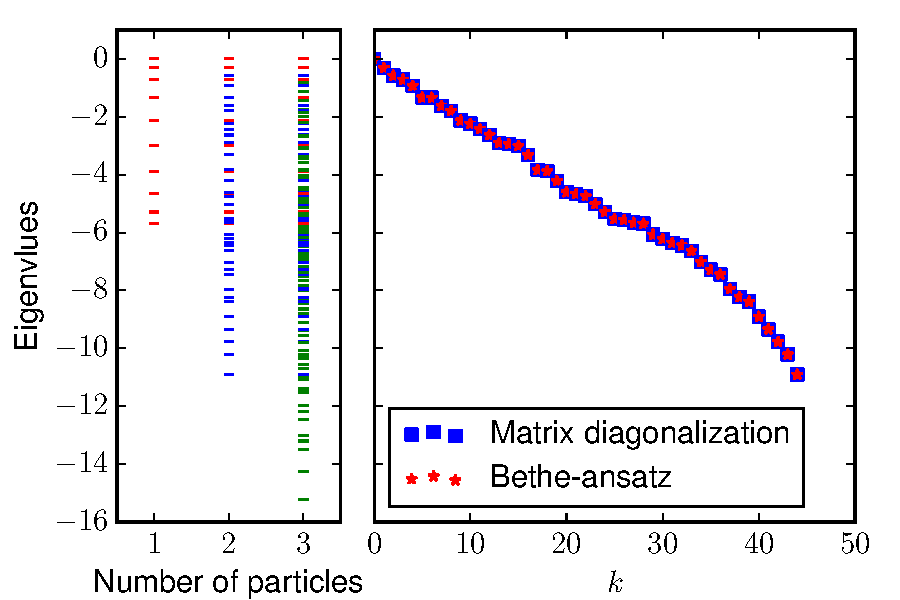
\includegraphics[width=0.8\linewidth]{spectrum}
%     \caption{Left: embeding of eigenvalues; Right: benchmark of eigenvalues from
%         Bethe Ansatz theory to directly diagonalize transition matrix, $N=2$.
%         $L=10$, $\alpha=2$ and $\beta=1$ for both. }
%     \label{fig:spectrum}
% \end{figure}

Finally, we remark that the Bethe Equations have to be solved numerically in
most cases. However, there is a small set of non-stationary eigenvalue and
eigenvectors we can obtain analytically, which correspond to the case with
just one excitation mode. The results are summarized as following:  
\begin{subequations}
    \label{eq:eigenN}
    \begin{align}
        \label{eq:partEigenvaluesN}
        \Lambda_k  = 
        -(\alpha+\beta) + 2\sqrt{\alpha\beta}\cos(\frac{k\pi}{L});
        ~k=1,2,\dots, L-1  \\
        \label{eq:eigenvectorsN}
        \Psi_k(x_1, x_2, \cdots, x_N)  =  A \sum_{n=1}^N
        \left(\frac{\alpha}{\beta}\right)^{n-1} \phi_k(x_n)\prod_{m\neq n} 
         \left(\frac{\alpha}{\beta}\right)^{x_m}
    \end{align}
\end{subequations}
Notice that the set of eigenvalue is exact the single particle spectrum, and
again $\phi_k(x)$ is exactly the single particle eigenfunction.
Fortunately, the numerical evidence shows that the most interesting
eigenmode, i.e. the slowest relaxation mode, is contained in this set. 
We will discuss it in next section. 

\section{Relaxation Time}
\label{sec:relaxation_time}

The largest non-zero eigenvalue we found and verified by numerical results is 
\begin{equation}
    \label{eq:largestEigenvalue}
    \Lambda_1 = -(\alpha+\beta) +
    2\sqrt{\alpha\beta}\cos(\frac{\pi}{L})
\end{equation}
If $L \gg 1$, we can expand the cos term, obtain 
\begin{equation}
    \label{eq:largestEigenvalueExpanded}
    \Lambda_1 = -(\sqrt{\beta}-\sqrt{\alpha})^2 -
    \frac{\sqrt{\alpha\beta}\pi^2}{L^2}
\end{equation}
And the relaxation time can be calculated as 
\begin{equation}
    \label{eq:relaxationTime}
    \tau = -\frac{1}{\Lambda_1}
\end{equation}

There are several information we can read form Eq.
\eqref{eq:largestEigenvalueExpanded} and \eqref{eq:relaxationTime}. Firstly, we
can see the scaling $\tau \approx L^2$, which means the dynamical exponent of
the system is $2$. Secondly, as we can see from Eq.
\eqref{eq:largestEigenvalueExpanded}, the bigger difference between $\alpha$
and $\beta$, the smaller relaxation time we will get. This is also consistent
as one would expect. If we map back to the polymer model, the result here can
be compared with the prediction of Rouse theory. Unlike the prediction
from Rouse theory that relaxation time does not depend on external force, we
have here that stronger external force decreases the relaxation time. This
point highlight the fundamental difference between the infinite extensible bead
spring model and the rigid bead rod model which is of course finite extensible. 

In Fig.  \ref{fig:eigenvalues} shows all the eigenvalues of a system with
lattice size $L=10$, calculated by brute force diagonalizing the transition
matrix.  Lattice The number of particles on the lattice is ranging from $1$ to
$9$. The difficult to calculate larger lattice size $L$ lies on that the
dimension grow as $\binom{L}{N}$, and if we take $N=L/2$, the dimension of the
matrix will became a extremely large number very soon. 

% \begin{figure}[htpb]
%     \centering
%     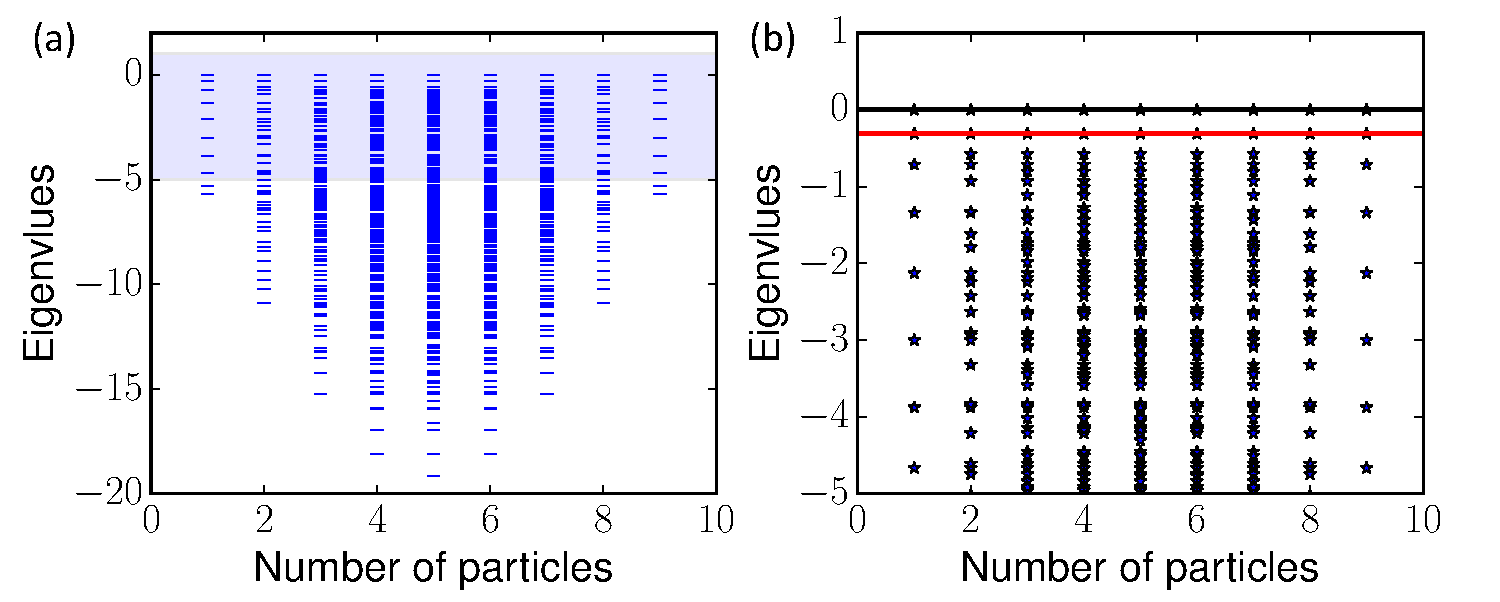
\includegraphics[width=0.8\linewidth]{eigenvalues}
%     \caption{Eigenvalues calculated by numerically diagonalize the transition
%         matrix.}
%     \label{fig:eigenvalues}
% \end{figure}

As we can see in Fig. \ref{fig:eigenvalues}
that all eigenvalues of case $N=1$ are contained in the set of
eigenvalues $N=2$, and all eigenvalues of case $N=2$ are contained in the set
of $N=3$ and so on until reach the largest set $N=L/2$. This means the
characteristic polynomial of $N=k+1$ always contains the factor of the
characteristic polynomial $N=k$. This is predict exactly by our theory. 

\section{Summary}
\label{sec:summeary}
We use the modified Bethe Ansatz methods solve the ASEP model with reflecting
boundaries.  The stationary distribution was solved exactly and the one
correspond to the relaxation time of the system was postulated. Numerical
evidence is provided for later statement.

\newpage

\appendix
\section{Derivation of the exclusion condition}
To derivate the exclusion condition, which is a little bit confusing at a first sight, we use the two particles example and then generalise to $N$ particle case.
First, let us rewrite the master equation of this two particle system:
\begin{equation}
    \begin{aligned}
        \label{eq:masterEqTwoGeneral}
    \frac{d P(x_1, x_2; t)}{dt} = & \alpha P(x_1-1,x_2;t) + \beta P(x_1+1,x_2;t) \\ 
    & + \alpha P(x_1, x_2-1; t) + \beta P(x_1, x_2+1; t)  \\ 
    & - 2(\alpha+\beta)P(x_1, x_2; t)
    \end{aligned}
\end{equation}
We assume the above equation is valid for the whole space. However, this is actually not true when the two particles are sitting on the neighboring sites. Let us now consider this special case separately, remember that $x_2 = x_1 + 1$. The master equation of this special case can be written as
\begin{equation}
    \begin{aligned}
        \label{eq:masterEqTwoNeighbor}
        \frac{d P(x_1, x_2; t)}{dt} = 
        & \alpha P(x_1-1,x_2;t) + \beta P(x_1, x_2+1; t)  \\ 
    & - (\alpha+\beta)P(x_1, x_2; t)
    \end{aligned}
\end{equation}
Now, let us do a subtraction, i.e. \eqref{eq:masterEqTwoGeneral} $-$ \eqref{eq:masterEqTwoNeighbor}, obtain
\begin{equation}
    \alpha P(x_1, x_2-1; t) + \beta P(x_1 + 1, x_2; t) = (\alpha + \beta)P(x_1, x_2; t)
\end{equation}
Let us then denote $x:=x_1$ and plug in $x_2 = x_1+1 = x+1$ in the above equation. We finally arrive at
\begin{equation}
    \label{eq:exclusionConditionTwo}
    \alpha P(x, x; t) + \beta P(x+1, x+1; t) = (\alpha + \beta)P(x, x+1; t)
\end{equation}

In summary, the sole master equation Eq. \eqref{eq:masterEqTwoGeneral} does not take into account the exclusion cases. In order to represent the exclusive setting, we assume Eq. \eqref{eq:masterEqTwoGeneral} is valid for the whole space, and then apply an additional condition on this equation like Eq. \eqref{eq:exclusionConditionTwo}. This condition is similar to the partial derivative of the PDF is the same at the collision boundary $x_1 = x_2$ in the continuous space case. 

Finally, in the similar way we can derive the exclusion condition for the cases $N>2$. However, it is not difficult to check that in cases of more than two particles, the three body collision or four body collision cases do not give out new conditions, just the linear combination of the two body collision conditions like Eq. \eqref{eq:exclusionConditionTwo}. This is fundamentally a result of Yang-Baxter Equation is satisfied for the ASEP model.




\subsection{Solution of General $N$ particles}
\label{sub:solution_of_general_n_particles}

\subsection{Relaxation Time}
\label{sub:relaxation_time}




%********************************** % Fourth Section  *************************************

\section{Relaxation Time of 3D Pinned Bead-rod Loop}
\label{sec:relaxation_time_of_3d_pinned_bead_rod_loop}


%********************************** % Fifth Section  *************************************
\section{The Single-file Diffusion}
\label{sec:the_single_file_diffusion}



%********************************** % Sixth Section  *************************************
\section{Summary}
\label{sec:summary}

\chapter{Characterize the Nuclear Oscillation}
\graphicspath{{Chapter5/Figs/}}

%********************************** %First Section  **************************************
\section{Oscillation of the Pinned Polymer Loop}
\label{sec:oscillation_of_the_pinned_polymer_loop}

\subsection{The Rouse Theory}
\label{sub:the_rouse_theory}

\subsection{Simulation Results}
\label{sub:simulation_results}




%********************************** %Second Section  *************************************
\section{Characterize the Shape of Chromosomes}
\label{sec:characterize_the_shape_of_chromosomes}

\subsection{The Gyration Tensor}
\label{sub:the_gyration_tensor}

\subsection{Asphericity and the Nature of Asphericity}
\label{sub:asphericity_and_the_nature_of_asphericity}



%********************************** % Third Section  *************************************

\section{Extract Shape Information From Experimental Data}
\label{sec:extract_shape_information_from_experimental_data}

\subsection{Shape from Experimental Data}
\label{sub:shape_from_experimental_data}

\subsection{Compare to Theory and Simulation Results}
\label{sub:compare_to_theory_and_simulation_results}


%********************************** % Fourth Section  *************************************
\section{Summary}
\label{sec:summary}




\chapter{Conclusions and Outlook}  
\graphicspath{{Chapter6/Figs/}}


%********************************** %First Section  **************************************

\section{Conclusions}
\label{sec:conclusions}



%********************************** %Second Section  *************************************

\section{Outlook}
\label{sec:outlook}








% ********************************** Back Matter *******************************
% Backmatter should be commented out, if you are using appendices after References
%\backmatter

% ********************************** Appendices ********************************

\begin{appendices} % Using appendices environment for more functunality


% ******************************* Thesis Appendix A ****************************
\chapter{An efficient algorithm to compute \emph{pseudo} force of bead-rod loop} 
\label{append:algorithm_bead_rod}

We have mentioned that the calculation of \emph{pseudo} force in the simulation is time consuming. In fact, the plain algorithm without optimization takes about $80\%$ of the simulation time. Thus we develop a efficient algorithm to calculate the \emph{pseudo} force. Recall that
\begin{equation}
    \label{eq:pseudoForceRecall}
    \mathbf{F}_i^{pseudo} = -\frac{1}{2} k_B T \sum_{\alpha, \beta} G_{\beta, \alpha}^{-1} \frac{\partial G_{\alpha\beta}}{\partial \mathbf{r}_i}.
\end{equation}
And $G$ is the metric matrix shown in Eq.~\eqref{eq:metricMatrix}. Notice that $G$ is a symmetric matrix with constant diagonal elements. 
The summation in Eq.~\eqref{eq:pseudoForceRecall} can be reduced to the summation of terms with $c_1, c_2, \cdots, c_L$ where $c_j = -\mathbf{u}_j \cdot \mathbf{u}_{j-1}$. Thus we can rewrite Eq.~\eqref{eq:pseudoForceRecall} as
\begin{equation}
    \label{eq:pseudoForceRewrite}
    \mathbf{F}_i^{pseudo} =  k_B T \sum_{j=1}^L G_{j-1,j}^{-1} \frac{\partial \mathbf{u}_{j}\cdot\mathbf{u}_{j-1}}{\partial \mathbf{r}_i}.
\end{equation}
Again, the periodic indexing is applied for $G_{j-1,j}^{-1}$. The derivative in the sum term of Eq.~\eqref{eq:pseudoForceRewrite} can be evaluated as 
\begin{equation}
    \frac{\partial \mathbf{u}_j }{\partial \mathbf{r}_i} = \frac{1}{a} (\delta_{i,j} - \delta_{i,j-1})(\mathbf{I} - \mathbf{u}_j\mathbf{u}_j),
\end{equation}
where $\mathbf{I}$ is the unit tensor. According to Cramer's rule, we can write
\begin{equation}
    G_{j-1,j}^{-1} = \frac{\text{cof}~G_{j,j-1}}{\det G},
\end{equation}
and $\text{cof}~G_{j,j-1}$ is the cofactor of $G_{j, j-1}$, which is the minus determinant of a $L-1\times L-1$ sub-matrix. So now we reduce the problem to the calculation of the determinant of a matrix. 

To calculate $\det\mathbf{G}$, let us first expand matrix $\mathbf{G}$ by the last line, obtain
\begin{equation}
    \label{eq:detGexpand}
    \det G = -c_L^2 \det\mathbf{S}_1 - c_{L-1}^2 \det\mathbf{S}_2 - 2(-1)^L\prod_{j=1}^L c_j + 2\det \mathbf{S}_3,
\end{equation}
where $\mathbf{S}_1,~\mathbf{S}_2,~\mathbf{S}_3$ are symmetric tridiagonal sub-matrices of $\mathbf{G}$. $\mathbf{S}_1$ is a $L-2\times L-2$ sub-matrix started with off-diagonal element $c_2$, $\mathbf{S}_2$ is a $L-2\times L-2$ sub-matrix started with $c_1$ and $\mathbf{S}_3$ is a $L-1 \times L-1$ sub-matrix started with $c_1$.

For a symmetric tridiagonal matrix, an efficient algorithm can be employed to calculate the determinant~\cite{Pasquali2002}. Let $\mathbf{S}$ be a $N\times N$ symmetric tridiagonal matrix with diagonal elements $d_1, d_2, \cdots, d_N$ and off-diagonal elements $s_1,s_2, \cdots, s_{N-1}$. Denote $\mathbf{T}^j$ the top left sub-matrix of $\mathbf{S}$ with $j$ rows and $j$ columns and $\mathbf{B}^j$ the bottom right sub-matrix of $\mathbf{S}$ with $N-j$ rows and $N-j$ columns. Then we have
\begin{subequations}
    \begin{align}
        \det \mathbf{T}^{j+1} & = d_{j+1} \det \mathbf{T}^j - s_{j}^2 \det \mathbf{T}^{j-1},\\
        \det \mathbf{B}^{j-1} & = d_{j-1} \det \mathbf{B}^j - s_{j-1}^2 \det \mathbf{B}^{j+1}.
    \end{align}
\end{subequations}
Notice that $\mathbf{T}^0 = \mathbf{B}^{N+1} = \mathbf{I}$ and $\mathbf{S} = \mathbf{T}^N = \mathbf{B}^0$. Use this algorithm and Eq.~\eqref{eq:detGexpand}, $\det\mathbf{G}$ can be calculate efficiently. 

Finally, the cofactor $\text{cof} G_{j,j-1}$, which is essentially a determinant, can be calculated as the same way as $\det\mathbf{G}$.
Use the algorithm above, the computation time of \emph{pseudo} can be reduced to $15\%$ of the total simulation time.


% ******************************* Thesis Appendix B ********************************
\chapter{Monte-Carlo simulation of 1D particle-lattice model}
\label{append:mc1D}


The Monte-Carlo simulation technique is widely used to study the particle-lattice model. In equilibrium, the standard simple Monte-Carlo algorithm can be applied to sample the stationary measure. However, what we discuss here is the Kinetic Monte-Carlo algorithm~\cite{Gillespie1976}. This algorithm allows us to go beyond equilibrium to the dynamics. We list in the following the main steps of the algorithm.

$\bullet$ Step 1: set the initial time $t=0$ and choose a initial state of the system. The initial state can be $N$ particle randomly distributed over $L$ lattice sites or other specified configurations. For the continence of later discussion, we denote the initial state as state $k$.

$\bullet$ Step 2: find all the possible hopping events and the corresponding hopping rates of the system. Let us denote the total number of hopping events as $N_k$ and the transition rate to a new state $i$ as $r_{ki}$. For example, if both sides of the $j^{\rm{th}}$ particle are empty sites, then two possible events are this particle hops to right or left. And the corresponding hopping rates are $\alpha$ or $\beta$, respectively. Notice that, the reflecting boundaries are specified here in the simulation. If the first particle is already sitting on first lattice site, then the hopping rate for it to the left is zero. And similar setting applies for the $N^{\rm{th}}$ particle. 

$\bullet$ Step 3: order the possible hopping events in a list and calculate the cumulative hopping rate $R_{ki} = \sum_{j=1}^i r_{ki}$ for $i=1, \cdots, N_k$. The total hopping rate is $Q_k := R_{kN_k}$.

$\bullet$ Step 4: draw a uniform random number $u\in(0,1]$. And find out the corresponding event $i$ that $R_{k,i-1} < uQ_k \leqslant R_{ki}$.

$\bullet$ Step 5: update the system from state $k$ to state $i$. 

$\bullet$ Step 6: update the system with $t = t + \Delta t$. Here, $\Delta t$ is drawn from the Poisson distribution, which can be calculated as 
\begin{equation}
    \Delta t = \frac{1}{Q_k} \ln\left(\frac{1}{u^{\prime}}\right),
\end{equation}
where $u^{\prime}$ is new uniform random number $u^{\prime}\in(0,1]$ that different from $u$. 

$\bullet$ Step 7: return to step 2 and do the iteration.

One have to wait for the system to reach equilibrium if the equilibrium statistics are the main interests. Usually the simulation runs quite fast. For a system of $1000$ lattice sites and $500$ particles, $10^6$ update steps take less than $10$ minutes.


% ******************************* Thesis Appendix C ********************************
\chapter{The Toeplitz matrix}
\label{append:teoplitz_matrix}

Toeplitz matrices are a special type of matrices that all elements along each diagonal parallel to the main diagonal are the same. Here, we focus on the tridiagonal Toeplitz matrix shown in Eq.~\eqref{eq:connectMatrix}.

To calculate the eigenvalues of matrix Eq.~\eqref{eq:connectMatrix}, we have to solve the equation 
\begin{equation}
    (\mathbf{A} - \lambda \mathbf{I}) \mathbf{x} = \mathbf{0}.
\end{equation}
Then we can obtain $L-1$ a set of linear difference equations such that
\begin{equation}
    \label{eq:differenceEqs}
    x_{j-1} - (2-\lambda)x_j + x_{j+1} = 0,~j=1,\cdots, L-1.
\end{equation}
And $x_0 = x_L = 0$ is set. The characteristic equation for the linear difference equation is
\begin{equation}
    \label{eq:characteristicEq}
    r^2 - (2-\lambda) r + 1 = 0.
\end{equation}
Let us denote the two roots of Eq.~\eqref{eq:characteristicEq} as $r_1,~r_2$. Then the solution of Eq.~\eqref{eq:differenceEqs} can be written as
\begin{equation}
    x_j = \left\{
    \begin{array}{ll}
        \alpha r_1^j + \beta r_2^j & \text{if  } r_1 \neq r_2,\\
        \alpha \rho^j + \beta j\rho^j & \text{if  } r_1 = r_2 = \rho,
  \end{array} 
  \right.
\end{equation}
where $\alpha$ and $\beta$ are arbitrary constants. The case of $r_1 = r_2$ can be eliminated because the resulting solution $x_0 = x_2 = \cdots = x_L = 0$ is trivial. Hence we have $x_j = \alpha r_1^j + \beta r_2^j$. Plug it into the boundary condition $x_0 = x_L = 0$ we obtain
\begin{subequations}
    \begin{align}
        \alpha + \beta & = 0, \\
        \alpha r_1^L + \beta r_2^L & = 0.
    \end{align}
\end{subequations}
From the above equations we can obtain $r_1 = r_2 \exp(i 2\pi k /L)$ for some $k = 1, 2, \cdots, L-1$. On the other hand, we can obtain from the Eq.~\eqref{eq:characteristicEq} that
\begin{subequations}
    \begin{align}
        r_1 r_2 & = 1, \\
        r_1 + r_2  & = 2-\lambda.
    \end{align}
\end{subequations}
Therefore, we can solve $r_1 = \exp(i \pi k /L)$ and $r_2 = \exp(-i \pi k/L)$. And the eigenvalues of $\mathbf{A}$ can be written as
\begin{equation}
   \lambda_k = 4\sin(\frac{k\pi}{2L}),~k=1, 2,\cdots, L-1.
\end{equation}
And the corresponding normalized eigenvectors are
\begin{equation}
    \mathbf{x}_k = 
        \begin{pmatrix}
            \sqrt{\frac{2}{L}}\sin\left(\frac{k\pi}{L}\right) \\
            \sqrt{\frac{2}{L}}\sin\left(\frac{2k\pi}{L}\right) \\
            \sqrt{\frac{2}{L}}\sin\left(\frac{3k\pi}{L}\right) \\
            \vdots\\
            \sqrt{\frac{2}{L}}\sin\left(\frac{(L-1)k\pi}{L}\right) \\
            
        \end{pmatrix}.
\end{equation}





% ******************************* Thesis Appendix D ********************************
\chapter{The Toeplitz Matrix}
The Toeplitz M


% ******************************* Thesis Appendix E ********************************
\chapter{Bethe equations of the periodic ASEP}
\label{append:bethe_equation_periodic_asep}

The ASEP model with periodic boundaries is the most simplest model that was solved long ago~\cite{Bethe1931,Mallick2011b}. The governing equation and exclusion condition are the same as the case of reflecting boundaries, shown in Eq.~\eqref{eq:masterEqN} and Eq.~\eqref{eq:exclusionConditionN}. The periodic boundary conditions can be written as
\begin{equation}
    \label{eq:periodicBoundaries}
    \Psi(x_1, x_2,\cdots,x_{N-1} x_N) = \Psi(x_2, x_3, \cdots, x_N, x_1 + L).
\end{equation}
The Bethe ansatz of periodic ASEP is constructed by the standard plane waves, which can be written as 
\begin{equation}
    \label{eq:betheAnsatzPeriodic}
    \Psi(x_1, x_2,\cdots, x_N) = \sum_{\sigma\in{S}_N} A_{\sigma} \prod_{n=1}^N \exp\left[ip_n x_{\sigma(n)}\right],
\end{equation}
where ${S}_N$ is the group of $N$-permutation, and $A_{\sigma}$ is the amplitude of the waves. $p_n$ is the wave vectors and $x_{\sigma(n)}$ is the position of the $\sigma(n)^{\rm{th}}$ particle.

By applying the exclusion condition Eq.~\eqref{eq:exclusionConditionN} and the periodic boundary condition Eq.~\eqref{eq:periodicBoundaries}, we can derive the following set of Bethe equations
\begin{equation}
    \label{eq:betheEqsPeriodic}
    e^{ip_n L} = (-1)^{N-1} \prod_{m\neq n}^N \frac{a(p_n, p_m)}{a(p_m, p_n)},
\end{equation}
where $a(p, p^{\prime}) = \sqrt{\alpha\beta}e^{i(p+p^{\prime})} - (\alpha+\beta) e^{ip} + \sqrt{\alpha\beta}$. 

By solving the Bethe equations, the wave vectors $p_n$ can be obtained. Then the eigenvalues of the system can be calculated as 
\begin{equation}
    \Lambda = \sum_{n=1}^N \left[-(\alpha+\beta) +2\sqrt{\alpha\beta}\cos(p_n)\right].
\end{equation}



% ******************************* Thesis Appendix D ********************************
\chapter{Single-file Diffusion with Reflecting Boundaries}
To derivate the exclusion condition, which is a little bit confusing at a first sight, we use the two particles example and then generalise to $N$ particle case.
First, let us rewrite the master equation of this two particle system:
\begin{equation}
    \begin{aligned}
        \label{eq:masterEqTwoGeneral}
    \frac{d P(x_1, x_2; t)}{dt} = & \alpha P(x_1-1,x_2;t) + \beta P(x_1+1,x_2;t) \\ 
    & + \alpha P(x_1, x_2-1; t) + \beta P(x_1, x_2+1; t)  \\ 
    & - 2(\alpha+\beta)P(x_1, x_2; t)
    \end{aligned}
\end{equation}
We assume the above equation is valid for the whole space. However, this is actually not true when the two particles are sitting on the neighboring sites. Let us now consider this special case separately, remember that $x_2 = x_1 + 1$. The master equation of this special case can be written as
\begin{equation}
    \begin{aligned}
        \label{eq:masterEqTwoNeighbor}
        \frac{d P(x_1, x_2; t)}{dt} = 
        & \alpha P(x_1-1,x_2;t) + \beta P(x_1, x_2+1; t)  \\ 
    & - (\alpha+\beta)P(x_1, x_2; t)
    \end{aligned}
\end{equation}
Now, let us do a subtraction, i.e. \eqref{eq:masterEqTwoGeneral} $-$ \eqref{eq:masterEqTwoNeighbor}, obtain
\begin{equation}
    \alpha P(x_1, x_2-1; t) + \beta P(x_1 + 1, x_2; t) = (\alpha + \beta)P(x_1, x_2; t)
\end{equation}
Let us then denote $x:=x_1$ and plug in $x_2 = x_1+1 = x+1$ in the above equation. We finally arrive at
\begin{equation}
    \label{eq:exclusionConditionTwo}
    \alpha P(x, x; t) + \beta P(x+1, x+1; t) = (\alpha + \beta)P(x, x+1; t)
\end{equation}

In summary, the sole master equation Eq. \eqref{eq:masterEqTwoGeneral} does not take into account the exclusion cases. In order to represent the exclusive setting, we assume Eq. \eqref{eq:masterEqTwoGeneral} is valid for the whole space, and then apply an additional condition on this equation like Eq. \eqref{eq:exclusionConditionTwo}. This condition is similar to the partial derivative of the PDF is the same at the collision boundary $x_1 = x_2$ in the continuous space case. 

Finally, in the similar way we can derive the exclusion condition for the cases $N>2$. However, it is not difficult to check that in cases of more than two particles, the three body collision or four body collision cases do not give out new conditions, just the linear combination of the two body collision conditions like Eq. \eqref{eq:exclusionConditionTwo}. This is fundamentally a result of Yang-Baxter Equation is satisfied for the ASEP model.





\end{appendices}

% ********************************** Bibliography ******************************
\begin{spacing}{0.9}

% To use the conventional natbib style referencing
% Bibliography style previews: http://nodonn.tipido.net/bibstyle.php
% Reference styles: http://sites.stat.psu.edu/~surajit/present/bib.htm

% \bibliographystyle{apsrev4-1}
% \bibliographystyle{plain}
\bibliographystyle{unsrt}
%\bibliographystyle{unsrt} % Use for unsorted references  
%\bibliographystyle{plainnat} % use this to have URLs listed in References
\cleardoublepage
% \bibliography{References/references} % Path to your References.bib file
\bibliography{/Users/wenwen/Documents/MendeleyDocs/library.bib} % Path to your References.bib file


% If you would like to use BibLaTeX for your references, pass `custombib' as
% an option in the document class. The location of 'reference.bib' should be
% specified in the preamble.tex file in the custombib section.
% Comment out the lines related to natbib above and uncomment the following line.

% \printbibliography[heading=bibintoc, title={References}]


\end{spacing}


% *************************************** Index ********************************
\printthesisindex % If index is present

\end{document}
